\documentclass[uplatex,dvipdfmx]{jlreq}

\usepackage{jlreq-deluxe}
\usepackage[noalphabet,hiragino-highsierra-pron]{pxchfon}
\usepackage[T1,LGR]{fontenc}
\usepackage{stix2}
\usepackage{roboto}
\usepackage[scale=0.95]{roboto-mono}

\usepackage[fleqn,tbtags]{mathtools} % 数式関連 (w/ amsmath)
\usepackage[dvipdfmx]{graphicx}
\usepackage{pxrubrica} 	% ルビを振るのに採用
\usepackage{tcolorbox}
\tcbuselibrary{listings,skins,breakable} % tcolorboxのオプション
\usepackage{ascmac} 	%screen/itembox/shadebox環境

\usepackage{listings,plistings}
\lstset{%
aboveskip=0pt,
belowskip=0pt,
language={[LaTeX]TeX}, 
morekeywords={tcbuselibrary, hypersetup, setlightminchofont, 
setmediumminchofont, setboldminchofont, setmediumgothicfont, 
setboldgothicfont, setxboldgothicfont, setmarugothicfont,
appendix, maketitle, textmc, textgt, textmg, mcfamily,
gtfamily, mgfamily, ebseries},
backgroundcolor={},% 
basicstyle={\small\ttfamily},% 
keywordstyle=\color{blue}\bfseries,
commentstyle=\color{red},
breaklines=true}

\usepackage[dvipdfmx]{hyperref}
\hypersetup{%
 bookmarksnumbered=true,%
 colorlinks=true,%
 linkcolor=magenta,
 citecolor=blue,
 urlcolor=blue}
\usepackage[dvipdfmx]{pxjahyper} % (u)pLaTeXのときは必要
\usepackage{hira-stix} 	% ヒラギノフォント&STIX2 代替フォント定義(Warning回避)

\newcommand{\mcbf}[1]{{\mcfamily\bfseries #1}}
\newcommand{\gtbf}[1]{{\sffamily\bfseries #1}}
\newcommand{\sfpi}{{\robotolgr p}}

\title{
\centering
\gtbf{情報工学科の{\TeX}の設定とサンプルファイルについてtetetetetetetetet}
}
\author{\mgfamily 佐波孝彦}
\date{\sffamily\small\today}

\renewcommand\UrlFont{\color{blue}\rmfamily}

\begin{document}
\maketitle

%\begin{titlepage}
%\vspace*{3cm}
%\centering
%\Huge\textsf{Title of Report}\\[2cm]
%\Large\textsf{情報工学科 1年}\\
%\Large\textsf{25G1000}\\[5pt]
%\huge\textsf{工大 太郎}\\[1cm] 
%\Large\textsf{\today}
%\end{titlepage}
%\clearpage

\section{はじめに}

{\TeX}(テフあるいはテックと読む)とは,コンピュータ科学者
Donald E.\ Knuth \cite{Knuth}が1978年に公開を始めた文書整形処理システムである.
印刷業界の用語では,組版処理システムとも呼ばれ,
用意した原稿素材(テキスト・図版・写真等)を各言語のルール\cite{JIS}\cite{typst}の下に,
指定のレイアウトになるように配置するソフトウェアである.
{\TeX}を用いると,OS(Operating System)に依存せずに出力結果の見た目を統一でき,
特に数式の仕上がりが綺麗なため,科学技術の分野では多くの出版物で利用されている.

情報工学科では,BYOD(Bring Your Own Device)の機種としてAppleのMacBook Air/Proを
指定しており,課題等の文書作成には{\TeX}を使うことを原則としている.
そのため,学科独自の設定を盛り込んだ,{\TeX}の設定スクリプトを用意しているが,
本稿は提出物作成の際に使用する標準的な書式のテンプレートを用いたサンプルであり,
学科独自の設定の概略を説明するものである.
{\TeX}の使い方そのものを説明する文書ではなく,あくまでテンプレート代わりの
サンプルとして用意したものである.とはいえ,数多くのコマンドを意図的に使っているため,
様々な場面で参考になるはずである.是非,活用して欲しい.
なお,添付している本稿のソースファイルでは,高度な設定を必要とするものを
省略しているため,コンパイルしてもこのPDF(Portable Document Format)ファイルと同一の見た目にはならいないことを
予めお断りしておく.

{\TeX}は,HTML(HyperText Markup Language)のようなマークアップ言語の一種である.
したがって,そのソースファイル(拡張子は\texttt{.tex})は,文章そのものと文章の構造や
見た目を指定するコマンドから成るテキストファイルである.複雑な数式や記号もテキストで入力する.
例えば,ギリシャ文字の$\pi$は,「ぱい」を変換してπとする(和文フォントが使われてしまう)のではなく,\verb|\pi|と入力する.単なるテキストファイルであるためOSに依存せず作成・編集でき,コンパイルすることによりファイル中のコマンドに基づいて文書が組版される.
組版結果はDVI(\textbf{\textsf{d}}e\textbf{\textsf{v}}ice-\textbf{\textsf{i}}ndependent)形式のファイル(拡張子は \texttt{.dvi})に書き出される.
DVIファイルは,表示デバイスやプリンタなどの装置に依存しない中間形式のバイナリデータであり,
DVIドライバと呼ばれる別のソフトウェア(DVIウェアとも言う)で組版結果をプレビューしたり,印刷可能なPostScript\cite{PS}ファイルに変換したりして利用する.また,近年ではDVIファイルをPDF\cite{PDF}に変換して,PDFファイルを最終出力とするのが一般的である.

{\TeX}はオープンソースソフトウェアであるため,組版処理を行うエンジンには,いくつもの派生系が存在している.中でも,複雑になりがちな各種の設定をマクロファイル(クラスファイルとパッケージファイルがある)を読み込むことで簡易に行える{\LaTeX} \cite{latex}がLeslie B.\ Lamport によって開発されて以降は,{\TeX}と言えば{\LaTeX}を指していることが普通である.
ただし,{\LaTeX}にも多くの派生エンジンが存在し,
日本では,縦書きや禁則処理などの日本語固有の処理を扱えるようにした{p\LaTeX}\cite{ptex},
さらに近年のOSで主流となったUnicode対応フォント(OpenTypeフォント)\cite{unicode}\cite{opntyp}を扱えるようにした{up\LaTeX} \cite{uptex}が長いこと主流である.世界的には,Unicode対応フォントを柔軟に扱え,かつ組版結果を直接PDFに出力できる{Lua\LaTeX} \cite{luatex}が主流になりつつあり,日本語を扱える{Lua\TeX-ja} \cite{luatexj}も日々進化している.ただし,{up\LaTeX}と{Lua\TeX-ja}はコマンド体系に違いがあるため,{Lua\TeX-ja}では{up\LaTeX}のソースコードをそのままコンパイルできない.
将来的には日本でも{Lua\LaTeX}が主流になることが予想されているが,現状では出版社や学術団体が用意しているマクロファイルの多くが{(u)p\LaTeXe}に基づいているため,本稿でも{\gtbf {up\LaTeX}の使用を前提}として説明をしていく.独学で学ぶ意欲のある方は,最初から{Lua\TeX-ja}を使っていくのも良いであろう(インストールはされている).ただし,学科として設定を統一したり,テンプレートを配布するのは,仕上がりの文書の体裁を統一するためでもあるので,そのことには注意を払うべきである.


\section{フォントについて}

前節冒頭で「{\TeX}を使うとOSに依存せずに出力結果の見た目を統一できる」と書いたが,それには前提条件があり,出力するコンピュータに同じフォントがインストールされている場合に限定される.
予定されたフォントがインストールされておらず別のフォントが代用されると,文字幅等が変わるのでページレイアウト自体は同一でも文章の行数が変わったり,見た目の印象も変わったりする.
情報工学科が推奨するMac{\TeX}\cite{mactex}のインストーラを用いると,オープンソースの無償フォントが数多くインストールされる.デフォルトでは,欧文にKnuth博士がデザインしたComputer Modern(CM)フォント\cite{cm},和文に原ノ味フォント\cite{harano}が使用される.
\begin{figure}[b]
\begin{itembox}[l]{\gtbf{Mac{\TeX}}}
\small\sffamily\mgfamily
世界的に最も普及している{\TeX}のディストリビューションは{\TeX} Liveであり,多くのOSプラットフォームで利用できる.Mac{\TeX}は,macOSに特化した{\TeX} Liveのインストーラである.一方,{\TeX} Liveは,Homebrew \cite{homebrew}やMacPorts \cite{macports}といった
パッケージ管理ツールを用いてインストールすることも可能である.しかし,両者はインストール先のディレクトリが異なるため,混在させるとファイルの依存関係が崩れ,正しく動かない実行ファイルがでてきたりする.したがって,Mac{\TeX}でインストールを行ったのであれば,以降も{\TeX}の更新はMac{\TeX}を用いるか,移行するのであれば,PATHの設定を変更する必要がある.
\end{itembox}
\end{figure}

フォントは好みもあるが,一般に有償の和文フォントは,様々な状況において見た目のバランスに優れ,出力結果の品質が高いのに対し,無償の和文フォントは品質のばらつきが大きい(和文には数万文字を超える漢字があるため,文字数の少ない欧文フォントに比べて,デザイン調整に膨大な手間が必要となるからである).macOSの日本語環境で使用されるヒラギノフォントは,癖のない高品質な有償フォントであるため,多くの出版物に採用\footnote{高速道路の標識にもヒラギノ角ゴシックが採用されている.}されている.そこで,情報工学科の用意した{\TeX}の設定スクリプトでは\gtbf{和文フォントにヒラギノを使用}する設定にしている.

ところで,現在のレーザープリンタはPostScript(PS)対応あるいはPS互換であることが一般的である.PSプリンタは,フォントもベクトルデータとして処理する\footnote{インクジェットプリンタでは,インク滴が1つの点(ドット)となり,その点を連続して吹きつけて面を構成することで,文字やグラフィックを表現している.}ため,拡大・縮小印刷をしても綺麗に印刷される.また,よく使われるフォントはプリンタに内蔵しておくと印刷が速い(そうでない場合は,フォントデータを都度プリンタに送信する必要がある).初期のPostScript Level 1(PS1)プリンタ\footnote{世界(そして日本)初のPSプリンタはAppleのLaserWriterである.}では,欧文フォントにセリフ体のTimes,サンセリフ体のHelvetica,タイプライタ体のCourier Newのそれぞれでローマン体,イタリック体,ボールド体,ボールドイタリック体,加えて記号用のSymbolおよびZapf Dingbatsの基本14書体(Base 14 fonts)が搭載されていた\footnote{PostScript Level 2(PS2)プリンタでは,基本14書体に加え,セリフ体としてPalatino,Bookman,New Century Schoolbook,サンセリフ体としてHelvetica Narrow,Avant Gardeそれぞれのローマン体,イタリック体,ボールド体,ボールドイタリック体と,筆記体のZapf Chanceryを加えた基本35書体(Base 35 fonts)が搭載された.現在の主流は,PostScript 3プリンタ(Levelをつけない)であり136書体の欧文フォントが搭載されている.}.
これらの基本14書体はAcrobat Readerにも内蔵されている(フォントが埋め込まれていないPDFで代用フォントとして用いられる\footnote{最近のAcrobat Readerでは,HelveticaとTimesが,それぞれArialとTimes New Romanに置き換えられている.}).

一方,日本語に初対応したPostScript Level 2(PS2)プリンタでは,欧文のセリフ体とサンセリフ体に相当する明朝体とゴシック体(モリサワのリュウミンL-KLと中ゴシックBBB)の基本2書体が搭載された.その後,明朝体とゴシック体が2ウエイト(太ミンA101と太ゴB101)が追加になり,さらに丸ゴシック体(じゅん101)も搭載され,基本5書体と呼ばれた.これらのフォントは当初パッケージとしては販売されておらず,プリンタとフォントを一体購入し,パソコンの画面上では解像度の粗いスクリーンフォント\footnote{ビットマップフォントと呼ばれ,各文字をピクセルのオン・オフで表現する.一方,文字の輪郭を曲線(ベクトル)で表現するPSフォントは,アウトラインフォントと呼ばれる.}を使用し,印刷すると綺麗な仕上がりになるという使用法\footnote{パソコンの処理速度が遅く,アウトラインフォントを画面に直接描画できない事情もあった.}であった.
このような背景から,日本語を扱う(u)p{\LaTeX}でも標準では丸ゴシック体を除く4書体が使用されてきた(印刷時はプリンタ内蔵のフォントが使われた).現在主流のPostScript 3プリンタに搭載される和文フォントは,平成明朝W3と平成角ゴシックW5であることが多い.しかし,近年のパソコンは処理能力が飛躍的に向上し,画面上でもアウトラインフォントを直接描画できるようになったため,プリンタの搭載フォントによらず任意のフォントを使用して書類を作成し,印刷することが可能である.ただし,プリンタに搭載されていないフォントを使用すると印刷にかかる時間は増える.

\begin{figure}[b]
\begin{itembox}[l]{\gtbf{ウエイト}}
\small\sffamily\mgfamily
フォントの太さはウエイト(Weight)で表される.フォントベンダーにより太さの基準や呼び方に違いはあるが最大で10段階程度に分類される.ISOでは9段階に分類されており,それぞれ,W1: Ultra Light(極細,Thin),W2: Extra Light(特細,Ultra Light),W3: Light(細),W4: Semi Light(中細,Regular/Normal),W5: Medium(中),W6: Semi Bold(中太,Demi Bold),W7: Bold(太),W8: Extra Bold(特太,Ultra Bold),W9: Ultra Bold(極太,Black/Heavy)と呼ばれる.カッコ内は日本語やISO以外での慣例的な呼び方である.ただし,実際にはこの表記が当てはまらないフォント製品も数多くある.
\end{itembox}
\end{figure}

\section{本稿のソースファイルの中身}

それでは,具体的に本稿のソースファイル,\texttt{sample.tex}の中身を見ながら,どのように記述していくのかを見ていく.
{\LaTeX}のソースコードは「ドキュメントクラス」「プリアンブル」「ドキュメント環境」の3つから成る.\ajMaru{1} 初めにドキュメントクラスを宣言し,\ajMaru{2} 次にプリアンブルで文書に必要なパッケージを読み込み,\ajMaru{3} ドキュメント環境の中で文章を記述していく.{\LaTeX}を用いた文書作成では,どの派生エンジンを用いてもこれが基本となる.

\subsection{ドキュメントクラス}


ドキュメントクラスとは,{\LaTeX}で作成する「文書の種類」を意味し,コンパイルするソースファイル(この場合,{\ttfamily sample.tex})において\gtbf{必ず最初に指定}する必要がある.
それには以下の構文で記述する.
\begin{tcolorbox}[colback=blue!5!white,colframe=blue!70!black]
\begin{lstlisting}
\documentclass[オプション]{ドキュメントクラス}
\end{lstlisting}
\end{tcolorbox}
\noindent 代表的なドキュメントクラスを表\ref{dcls}に示す.

\begin{table}[bt]
\centering
\caption{よく使われるドキュメントクラス}\label{dcls}
\begin{tabular}{|l||l|l|l|l|l|} \hline
\textsf{\small 用途} & \textsf{\small 欧文(標準)}& \textsf{\small 和文(横書き)}& \textsf{\small 和文(縦書き)}& \textsf{\small 和文(新・縦横)}&\textsf{\small 和文(新・縦横)}\\\hline
{\small 論文・レポート} & article & \textcolor{lightgray}{jarticle} & \textcolor{lightgray}{tarticle} & jsarticle&\textcolor{red}{jlreq}\\
{\small 長い報告書} & report & \textcolor{lightgray}{jreport} & \textcolor{lightgray}{treport} & jsreport&{\small (オプション指定)}\\
{\small 本} & book & \textcolor{lightgray}{jbook} & \textcolor{lightgray}{tbook} & jsbook&{\small (オプション指定)}\\ \hline 
\end{tabular}
\end{table}



ドキュメントクラスは,文書の用途に応じた標準書式を定義するものであり,
文書のレイアウトや見出しなどの様式を作成者によらず共通にすることができる.
2列目と3列目のクラス(jclasses)は,{p\LaTeX}の初期の頃に作られた古いパッケージであり,
日本語組版の満たすべき標準的な要件を満たせないことが多い.そのため,現在では4列目のjsclassesパッケージ\cite{jscls}を使うのが一般的になったが,日本語組版処理の要件(Requirements for Japanese Text Layout)\cite{jlw3c}を満たすことを目指したjlreq \cite{jlreq}が登場して以降は,
そちらにトレンドが移りつつある\footnote{jsclassesは,標準のフォントサイズ(10pt)で使用する場合はよいが,
12ptなどを用いると長さの扱いが面倒になる.例えば,\texttt{\textbackslash hspace\{10cm\}}とすると12cmのスペースが空く.これは,縮小した用紙サイズで10ptのフォントサイズで組版してから最後に用紙全体を1.2倍に拡大してフォントサイズが12ptになるようにするという方式を採用しているためである.}.他にもjsclassesパッケージにおける(u)p{\LaTeX}依存の部分を無くし,Lua{\TeX}等でも使えるようにしたBXjsclsパッケージなどもあるが,\gtbf{授業の課題等で日本語のレポートを書く場合は,\textbf{\texttt{jlreq}}を使用}するのがよい.
ドキュメントクラスごとに指定するオプションでは,用紙サイズやフォントサイズなどを
指定するが,詳しくはjlreqのドキュメントを参照のこと.
\begin{screen}
\small\sffamily
ドキュメントクラスの設定では,指定していないオプションはデフォルトの値が使われる.
\end{screen}
\begin{screen}
\small\sffamily
{\TeX}は開発速度が速いので,インターネットや書籍などで情報を探したときに,\texttt{jarticle}などを指定しているものは,情報が古いだけでなく,現在では好ましくない方法の場合もあるので参考にすべきではない.なるべく最新のドキュメントを確認すべきである.
\end{screen}

なお,jlreqでは,使用する{\LaTeX}エンジンによって処理内容が異なる項目があるため,
クラスオプションで処理エンジンに{up\LaTeX}を使用することを明示しておく方がよい
(自動判別の機能もあるが,指定しておくことが推奨されている).
また,文字色をつける\texttt{xcolor}や図版や写真を埋め込む\texttt{graphicx}などの特定の
パッケージを使用する場合,DVIドライバを指定しないと期待通りの出力にならないことがあるが,
ドキュメントクラスのオプションはグローバルオプションとも呼ばれ,その内容が必要に応じて
他のパッケージにも伝達される.したがって,documentclassのオプションで DVI ドライバを
指定しておけば\texttt{xcolor}や\texttt{graphicx}などのパッケージを使う場合に,
いちいち同じ指定を繰り返す必要がなくなる.そのため,ここでDVIファイルをPDFに
変換するDVIドライバとして\texttt{dvipdfmx}を指定しておく.
標準的には以下の通りとなり,本稿でも同じ指定にしている.
\begin{tcolorbox}[colback=blue!5!white,colframe=blue!70!black]
\begin{lstlisting}
\documentclass[uplatex,dvipdfmx]{jlreq}
\end{lstlisting}
\end{tcolorbox}

\subsection{プリアンブル}

\subsubsection{パッケージの読み込み}

プリアンブルでは,実際の文書の内容を書き始める前に,本文中で使うコマンドやフォントの取り扱いなどが定義されたパッケージを指定したり,文書のタイトル情報などを入力する.パッケージに含まれない独自の定義などもここで行う.
プリアンブルにおけるパッケージの読み込みは以下の構文で行う.
\begin{tcolorbox}[colback=blue!5!white,colframe=blue!70!black]
\begin{lstlisting}
\usepackage[オプション]{パッケージ}
\end{lstlisting}
\end{tcolorbox}

パッケージは膨大な種類が開発されている(インストールされた「TeX Live ユーティリティ」の
パッケージのタブでその種類を確認できる)ので,その全てを把握することは不可能に近いが,
ここでは,本サンプルで採用したものを説明する.
本稿では以下のパッケージを読み込んでいる.
\begin{tcolorbox}[title=\gtbf{本稿で採用したパッケージ},colback=blue!5!white,colframe=blue!75!black,enhanced,breakable=true]
\begin{lstlisting}
\usepackage{jlreq-deluxe}
\usepackage[noalphabet,hiragino-highsierra-pron]{pxchfon}
\usepackage[T1,LGR]{fontenc}
\usepackage{stix2}
\usepackage{roboto}
\usepackage[scale=0.95]{roboto-mono}
\usepackage[fleqn,tbtags]{mathtools}     % 数式関連 (w/ amsmath)
\usepackage[dvipdfmx]{graphicx}
\usepackage[dvipdfmx]{xcolor}
\usepackage{pxrubrica}                   % ルビの機能
\usepackage{ascmac}                      % screen/itembox/shadebox環境
\usepackage{tcolorbox}                   % 様々な枠環境
\tcbuselibrary{listings,skins,breakable} % tcolorboxのオプション
\usepackage{listings,plistings}          % ソースコードの表示機能
\lstset{                                 % listingsのオプション
  aboveskip=0pt,
  belowskip=0pt,
  language={[LaTeX]TeX}, 
  morekeywords={% パッケージにコマンドや関数と認識されないものを列挙しておく.
                % 本例では和文用のコマンドなどを登録している.
  appendix, maketitle, textmc, textgt, textmg, mcfamily,
  gtfamily, mgfamily, ebseries},
  backgroundcolor={},% 
  basicstyle={\small\ttfamily},% 
  keywordstyle=\color{blue}\bfseries,
  commentstyle=\color{red},
  breaklines=true} 
\usepackage[dvipdfmx]{hyperref}
\hypersetup{%
  bookmarksnumbered=true,%
  colorlinks=true,%
  linkcolor=magenta,
  citecolor=blue,
  urlcolor=blue}
\usepackage[dvipdfmx]{pxjahyper}     % (u)pLaTeXのときは必要
\usepackage{hira-stix} % ヒラギノフォントの代替フォント定義(Warning回避)
\end{lstlisting}
\end{tcolorbox}

\begin{itemize}
\item{\sffamily\bfseries jlreq-deluxe パッケージ}は,(u)p{\LaTeX}でjlreqクラス
使用時に多書体(多ウエイト)の和文フォントを利用可能にするパッケージである\cite{jlreq-deluxe}.
予め明朝体で2ウエイト(細明朝(W3)と{\bfseries 中太明朝(W6)},ゴシック体で2ウエイト({\sffamily 細ゴシック(W3)},{\sffamily\bfseries 中太ゴシック(W6)},
さらに{\mgfamily 中細丸ゴシック(W4\footnote{アルファベットや数字は欧文フォントが使用されるが,丸ゴシック体に相当する欧文フォントの設定がない.そのため,このW4はセリフ体のフォントで表示されている.詳しくは次節参照.})}の計5書体が設定される.
実はこの機能は,日本語文書作成時に(u)p{\LaTeX}で OpenType フォント
(Unicode 対応フォント)を扱えるようにするOTFパッケージ\cite{OTF}のオプションで
deluxeを指定したときと同じである.
しかし,jlreqクラス使用時にOTFパッケージを利用すると,jlreqクラスの意図する組版結果が
得られなくなってしまう.そのためOTFパッケージとの互換性を保ちながら開発された.
オプションは,OTFパッケージと同じであるが,up{\LaTeX}で使用するなら特に指定する必要はない.

\item{\sffamily\bfseries pxchfon パッケージ}は,{p\LaTeX}/{up\LaTeX} $+$ dvipdfmxの環境で,
日本語文書で使える7書体(明朝体3ウエイト,ゴシック体3ウエイト,丸ゴシック体1ウエイト)をユーザ指定のフォントに設定するパッケージである\cite{pxchfon}.ただし,MacOSに内蔵されているヒラギノフォントは明朝が2ウエイト(W3とW6),ゴシックが10ウエイト(W0$\sim$W9),丸ゴシックが1ウエイト(W4)であるため,内蔵ヒラギノフォントを使う場合に設定できるのは6書体(細明朝(W3),\mcbf{中太明朝(W6)},{\sffamily 細ゴシック(W3)},\gtbf{中太ゴシック(W6)},{\gtfamily\ebseries 特太ゴシック(\robotoBlack{W8})}および{\mgfamily 中細丸ゴシック(\robotoRegular{W4})})のみとなる.
オプションに\texttt{hiragino-highsierra-pron}を指定すると,ヒラギノ6書体が使える設定になる.
なお,多書体を使うには,\gtbf{先にjlreq-deluxeパッケージを読み込んでおく必要がある}.
論文やレポートを書くときに使用する和文フォントはせいぜい2$\sim$3書体程度であるので,通常はjlreq-deluxeパッケージを使用するだけでもよい.

また,オプションには,\texttt{alphabet},\texttt{noalphabet},\texttt{relfont}(この3つは排他的で同時に使用できない)のいずれかを記述する.\texttt{alphabet}や\texttt{relfont}は,英数字部分も指定の和文フォントの英数字を使って表示する設定である.ただし,半角等幅の字体しか表示できない制約があり,見た目のバランスが良くない.したがって,通常は\texttt{noalphabet}(英数字に和文フォントを使用しない設定)にするのが一般的である.そうすることで,英数字部分はプロポーショナルな欧文フォントが使われ,数式ともバランスが取れる.

\item{\sffamily\bfseries fontenc パッケージ}は,フォントのエンコーディングを指定するパッケージであり\cite{fontenc},各種欧文フォントパッケージを使用するときに,オプションでエンコーディング方式を指定する.このパッケージで最も一般的なオプションであるT1は,欧州言語の文字のエンコーディングで,ほとんどのアクセント文字が定義される.他に,T1の拡張エンコーディングであるTS1,Knuth博士が作った{\TeX}のオリジナルの7ビットエンコーディングであるOT1,ギリシャ文字のエンコーディングであるLGR,
日本語の横書きと縦書き文字用のJY1とJT1(up\LaTeX を使う時はJY2/JT2,Lua\TeX-jaの場合はJY3/JT3にする),{\TeX}の数式用フォントを販売していたY\&Y社が定めたLY1などがあり\footnote{
{\TeX}のエンコーディングは命名規則があり,以下の文字で始まるエンコーディング名は予約されている.T(標準 256 文字のテキスト),TS (対応する T エンコーディングを拡張するように設計されたシンボルエンコーディング),X(T エンコーディングの厳密な要件に準拠しないテキストエンコーディング),M(標準 256 文字の数式用エンコーディング),S(その他のシンボルエンコーディング),A(その他の特殊なアプリケーション),OT(標準 128 文字のテキストエンコーディング),および OM(標準 128 文字の数式用エンコーディング).サイトまたはシステムにローカルなエンコーディング方式は L で始まり,広く配布することを目的とした実験的なエンコーディングは E で始まる.},使用するフォントに応じて変更あるいは追加する.
\begin{screen}
\small\sffamily
初期の欧文{\TeX}では符号空間が7ビット,すなわち1つのフォントで表せる文字は128種類しかなかった.そのため,初期のCMフォントは7ビットフォントであったが,その後,欧文{\LaTeX}では8ビットフォントが標準になり,現在では100万を超える欧文以外の文字も表せるUnicode対応フォントを扱える{\LaTeX}が普及している.ここでのエンコーディングとは,使用するフォントがどのような文字セットをもつフォントなのかを{\TeX}に伝えるもので,UTF-8のようなソースファイルの文字コードとは異なる.
\end{screen}

\item{\sffamily\bfseries stix2 パッケージ}は,欧文のセリフ体や数式に STIX(\gtbf{S}cientific and \gtbf{T}echnical \gtbf{I}nformation e\gtbf{X}change)Twoフォントを使用するためのパッケージである\cite{stix2}.
STIX Two フォントは,アメリカ数学会(AMS: American Mathematical Society)や米国電気電子学会(IEEE: Institute of Electrical and Electronics Engineers)を含む多くの学協会の出版物に
標準で使われるセリフ体フォントであり,Googleフォントにも採用されている.
一般に,数式は文字だけでなく特殊な記号等も必要になるため,通常のテキスト用フォントのみでは表現できないことがある.そこで,通常は数式部分に別のフォントを使用するが,その場合,本文のフォントと異なる字形になってしまう.STIX Twoフォントには,STIX Two TextとSTIX Two Mathの2つがあり,数式用にデザインされたフォントが含まれるため,本文のフォントとの整合性は完璧である.また,AMSの配布する数式記述用パッケージ(amsmath)にも対応しているため,それらのコマンドも問題なく使用できるのは大きな利点である.

ところで,STIX Two TextフォントはMacOSにも{\TeX}のディレクトリの中にも4ウエイト分がインストールされているが,{\TeX}で使えるようにするメトリックファイルは2ウエイト分しか用意されていない.ヒラギノの明朝体も2ウエイトのみなのでバランスは取れているが,{\TeX}で使えるのは,ローマン体,イタリック体,スモールキャピタル体がそれぞれ2ウエイト\footnote{レギュラーとボールドが使用されるが,それぞれヒラギノ明朝のW3とW6より若干太いのは気になる.\label{太い}}のみである.また,サンセリフ体やタイプライタ体がない(STIX Two Mathにはどちらもあるが,本文中で使うとバランスが悪い)ため,それらには別のフォントを指定する必要がある.

\item{\sffamily\bfseries roboto パッケージ}は,欧文のサンセリフ体に
Robotoフォントを使用するためのパッケージである\cite{roboto}.Robotoフォントは,Googleフォントにも採用されており,ヒラギノ角ゴシックともバランスが良いと思う.
オプションは指定しなくとも,サンセリフ体のみにRobotoが適用される.
また,ウエイトも6種類使える\footnote{STIX Twoと同様,デフォルトのレギュラーとボールドはヒラギノ角ゴシックのW3とW6より若干太いので,気になる場合はデフォルトの設定ウエイトを1つ下げればよい.本稿では個別に指定したW8の部分以外はそのままにしてある.\label{太い2}}
ので,パッケージで定義されているコマンド(\verb|\robotoThin{}|,\verb|\robotoLight{}|,\verb|\robotoRegular{}|,\verb|\robotoMedium{}|,\verb|\robotoBold{}|,\verb|\robotoBlack{}|)により個別にウエイトを指定することも可能である.
本稿では,pxchfon パッケージの説明で{\gtfamily\ebseries 特太ゴシック(\robotoBlack{W8})}のW8部分で個別に指定している.

\item{\sffamily\bfseries roboto-mono パッケージ}は,欧文のタイプライタ体に
等幅のRoboto Monoフォントを使用するためのパッケージである\cite{roboto}.オプションは特に指定しなくてよいが,デフォルトのままだと日本語フォント部分に比べてサイズが若干大きく感じるので,ここでは[scale=0.95]に調整している.



\item{\sffamily\bfseries mathtools パッケージ}は,数式を表現するための機能を提供するパッケージである\cite{mathtools}.従来より{\LaTeX}の数式用のパッケージとして,AMSの開発するamsmathパッケージが使われてきたが,mathtoolsはamsmathの不具合を修正した拡張パッケージである.mathtoolsを読み込むとamsmathパッケージも自動的に読み込まれるので,個別にamsmathを読み込む必要はない.
オプションには,amsmathのオプションを書くことも可能である.ここでは,数式の配置を文章幅の左右中央ではなく,左から一定の字下げの後で行う\texttt{fleqn}と,複数行に折り返す式を書く時の式番号が,番号を右側に配置するときは一番下,番号を左側に配置するときは一番上に配置される\texttt{tbtags}を指定している.mathtoolsやamsmathのオプションは多数あるので,詳しくはドキュメントを参照のこと.

\item{\sffamily\bfseries graphicx パッケージ}は,文書に画像を挿入したり,テキストや図の拡大・縮小・回転を行うためのパッケージである\cite{graphicx}.図はEPS(Encapsulated PostScript)あるいはPDFで用意し,写真であればPNG(Portable Network Graphics)あるいはJPG(Joint Photographic Experts Group)で用意しておく.{\TeX}そのものには画像を処理する機能はなく,画像を配置する領域を確保するだけであり,実際の処理はDVIウェアが行う.したがって,オプションには,DVIドライバの記述が必要である.また,\gtbf{写真は解像度を適切に下げて}おかないと最終的にできあがるPDFファイルのサイズがサーバ等のアップロードサイズの上限を超えることがあるので注意する.

\item{\sffamily\bfseries xcolor パッケージ}は,文字に色をつけるために使用するパッケージである\cite{xcolor}.オプションには,DVIドライバが必要である.

\item{\sffamily\bfseries pxrubrica パッケージ}は,日本語組版においてルビや圏点をつけるために使用するパッケージである\cite{pxrubrica}.オプションは存在しない.

\item{\sffamily\bfseries ascmac パッケージ}は.図や罫線で囲んだボックスを出力する命令などを提供するパッケージである\cite{ascmac}.詳細はドキュメントを参照のこと.

\item{\sffamily\bfseries tcolorbox パッケージ}は,文章などを枠で囲む機能を提供するパッケージである\cite{tcolorbox}.オプションが豊富にあるので,他のパッケージのように\verb|[ ]|の中に羅列すると非常に長くなることがある.その場合,別のコマンド\verb|\tcbuselibrary|を使って別に列挙する方が整理して記述できる.本稿では{\TeX}のソースを表示するときの枠に使用している.詳細はドキュメントを参照のこと.色などが関係するので\gtbf{graphicxやxcolorパッケージの後に読み込む}必要がある.以降のパッケージも同様である.

\item{\sffamily\bfseries listings パッケージ}は,文章中でプログラム言語の
ソースコードなどをリストする機能を提供するパッケージである\cite{listings}.指定した言語の関数部分を色付けするなどの機能ももつ.本稿では,{\TeX}のソース表示に使用している.
ただし,ソースの中に和文が含まれると正しく表示されないため,和文対応するための拡張パッケージ(jlisting,jvlisting,plistingsなどがある)も読み込む.オプションが豊富にあるので,別のコマンド\verb|\lstset|で列挙し,ここでは{\TeX}のコマンド定義の追加(和文用のコマンドが定義されていないため)や色の指定などをしている.詳細はドキュメントを参照のこと.

\item{\gtbf{hyperref パッケージ}}は,出力のPDFファイルに,HTMLと同様なハイパーリンク機能を加えるためのパッケージである\cite{hyperref}.PDFのしおり機能で目次をつけたり,URLへのリンクを指定したりすることができる.本稿では,目次を自動作成する機能と,リンクに色をつける設定を採用している.
オプションが豊富にあるので,\verb|\hypersetup|を使って列挙する.詳細はドキュメントを参照のこと.

\item{\gtbf{pxjahyper パッケージ}}は,(u){p\LaTeX} $+$ hyperref $+$ dvipdfmx の組み合わせで
日本語を含むPDFを作成する際,しおりの文字化けなどを解消するために使用するパッケージである\cite{pxjahyper}.
オプションも色々設定できるが,高度なことをしないなら読み込んでおくだけでよい.\gtbf{hyperrefパッケージの後に読み込む}こと.

\item{\sffamily\bfseries hira-stix パッケージ}は,ソースファイルのコンパイル時にフォント
関連のワーニングが多数表示されるのを回避するために,予め代替フォントを定義した独自パッケージである.
本稿で使用しているフォント(ヒラギノ,STIX Two,Roboto)は書体やウエイトに限りがあるため,ソースファイル上でこれらのフォントに含まれない書体の指定が現れると,指定のフォントがないため別のフォントで代用する旨を表示するワーニングメッセージが沢山表示される.
ワーニングメッセージが沢山あると,その他の部分にも問題があった場合に,問題箇所の識別が大変になるため,フォントに起因するワーニングメッセージの出現を回避するために簡易的に作成した.オプションはないので,ただ読み込むだけで良い.
\end{itemize}

以上が,本稿で使用しているパッケージの概要であるが,{\LaTeX}のパッケージは,まだまだ沢山ある.種類や使用法については各自で調べて欲しいが,慣れてくるとパッケージで読み込むスタイルファイルの中身を見ることで理解できることも多い.
パッケージファイルは\texttt{.sty}の拡張子をもつのが普通で,ターミナル上で簡単に検索できる.例えば,pxchfonパッケージであれば,実体はpxchfon.styなので,その場所は,
\begin{tcolorbox}[colback=blue!5!white,colframe=blue!70!black]
\begin{verbatim}
>> kpsewhich pxchfon.sty
/usr/local/texlive/2024/texmf-dist/tex/platex/pxchfon/pxchfon.sty
\end{verbatim}
\end{tcolorbox}
\noindent
のように検索できる(kpsewhichは{\TeX}によってインストールされるコマンドである).
ファイルの部分を除いて,
\begin{tcolorbox}[colback=blue!5!white,colframe=blue!70!black]
\begin{verbatim}
>> open /usr/local/texlive/2024/texmf-dist/tex/platex/pxchfon/
\end{verbatim}
\end{tcolorbox}
\noindent
とすればフォルダとして開けるので,テキストエディタなどでファイルの中身を見られる.
あるいは,ターミナル上で当該ディレクトリに移り,moreやlessコマンド等で見てもよい.

\subsubsection{独自の設定}

プリアンブルにはパッケージの読み込みだけでは設定しきれない,その他の設定を記述することもある.ここでは,pxchfonパッケージで使用する7書体(実際には重複があるので6種類であるが)を
自分で記述した場合の例を掲載している.
ここで,MacOSに内蔵のヒラギノフォントは,ゴシック体がウエイトごとに1つのファイルになっているのに対し,明朝体は1つのファイルに複数ウエイトを内包している.そのため,ウエイトに対応したフォントの番号の指定が必要となる.
ただし,これらの設定は自分で書かずとも\texttt{pxchfon-extras.def} \cite{PXex}というファイル
\footnote{\texttt{pxchfon-extras.def}は,ディストリビューションに含まれないため,別にダウンロードする必要がある.}を{\TeX}のディレクトリの中に置いておけば,pxchfonパッケージのオプションで,
\texttt{[hiragino-highsierra-pron]}と指定するだけで同じ設定が自動で読み込まれる.
情報工学科の設定スクリプトでは,\texttt{pxchfon-extras.def}がディレクトリにコピーされる.
\begin{figure}[b]
\begin{itembox}[l]{\gtbf{TLContrib}}
\small\sffamily\mgfamily
{\TeX}は書籍の付録としてDVDやUSBメモリなどに収録して配布されることもあり,利用や改変,商用再配布にライセンス上制約がないものだけがディストリビューションに含められている.
ところが,パッケージの一部のファイルには「商用・非商用を問わず無料で利用可能だが,商用再配布を禁じる」など,ライセンス上含められないものがある.
そのようなファイルや拡張パッケージを配布する目的でTLContrib(Contributed packages for TeX Live)というディストリビューション\cite{tlcontrib}が存在する.情報工学科の設定スクリプトでもTLContribから一部のファイルをダウンロードしている.
\end{itembox}
\end{figure}

\begin{tcolorbox}[colback=blue!5!white,colframe=blue!70!black,breakable=true]
\begin{lstlisting}
\setlightminchofont[0]{HiraginoSerif.ttc}	% \mcfamily\ltseries W3を指定
\setmediumminchofont[0]{HiraginoSerif.ttc} 	% \mcfamily\mdseries W3を指定
\setboldminchofont[2]{HiraginoSerif.ttc}	% \mcfamily\bfseries W6を指定
\setmediumgothicfont{HiraginoSans-W3.ttc}	% \gtfamily\mdseries
\setboldgothicfont{HiraginoSans-W6.ttc}		% \gtfamily\bfseries
\setxboldgothicfont{HiraginoSans-W8.ttc}	% \gtfamily\ebseries
\setmarugothicfont{HiraginoSansR-W4.ttc}	% \mgfamily
\end{lstlisting}
\end{tcolorbox}

なお,2節にも書いたが,日本語対応のPSプリンタは,当初2書体しか使用できなかったため,文章中で文字を{\gtfamily 強調}するときなどは書体を変える以外の選択肢がなかった.
5書体になり太字が使えるようになっても,明朝体での{\mcfamily\bfseries 強調}はゴシック体での{\gtfamily\bfseries 強調}に比べ,インパクトに欠けるため,現在でも日本語の文章では強調するときに,ゴシック体を用いることが一般的である.因みに,欧文の文章での強調はイタリック体にするのが一般的である.したがって,文字を強調するコマンド\verb|\emph{}|を使うと和文は細ゴシック体,欧文はイタリック体になる.

ただし,日本語の技術文章では,英数字と日本語が混在する用語や文章を書くことが多いため,
\verb|\emph{}|を使うことはほとんどない.
また,\verb|\textgt|コマンドで強調するのも,ゴシック体とセリフ体が混ざってしまいバランスが悪い.
例えば,pxchfonパッケージを強調したいとき,{\gtfamily\bfseries pxchfonパッケージ}とするよりも{\sffamily\bfseries pxchfonパッケージ}とする方が統一感があるし,統計学における
{\gtfamily\bfseries 68-95-99.7則}は,{\sffamily\bfseries 68-95-99.7則}とする方が
バランスが良い.これは,節見出しなどの節番号と見出しについても同じことが言える.
このことは気に留めておくべきである\footnote{
初期の{p\LaTeX}の時代には,ゴシック体のコマンドで,英数字も欧文フォントのサンセリフ体に
切り替える設定が良く使われたが,現在は今回採用しているパッケージのコマンドで簡単にできる.}.

\subsubsection{独自のコマンド}

プリアンブルには,独自のコマンドを定義しておくこともできる.
新しいコマンドは以下の構文で作成できる.
\begin{tcolorbox}[colback=blue!5!white,colframe=blue!70!black]
\begin{lstlisting}
\newcommand{\関数名}[引数の数]{関数の定義}
\end{lstlisting}
\end{tcolorbox}
\noindent
引数は\verb|#|番号を用いて,定義の中で記述する.

例えば,書体の指定などは組み合わせると長くなりがちなので,
ここでは例として以下の2つのコマンドを定義し,本稿でも使用している.
\begin{tcolorbox}[colback=blue!5!white,colframe=blue!70!black]
\begin{lstlisting}
\newcommand{\mcbf}[1]{{\mcfamily\bfseries #1}} %\mcbfという命令型コマンドを定義
\newcommand{\gtbf}[1]{{\sffamily\bfseries #1}} %\gtbfという命令型コマンドを定義
\end{lstlisting}
\end{tcolorbox}
\noindent
これらはそれぞれ,中太字明朝体,中太ゴシック体
(英数字は対応する欧文フォントのボールド体を使用)を指定する
コマンドになっている.また,既存のコマンドの定義を変更するには,\verb|\renewcommand|を使う.

\subsubsection{タイトルの出力}

作成する文書にタイトルを書く場合,入力はプリアンブル内で,
\begin{tcolorbox}[colback=blue!5!white,colframe=blue!70!black]
\begin{lstlisting}
\title{タイトルの中身}
\end{lstlisting}
\end{tcolorbox}
\noindent
と書き,\verb|\begin{document}|以降に\verb|\maketitle|と記述すれば,「タイトルの中身」がタイトルとして出力される.同様に

\begin{tcolorbox}[colback=blue!5!white,colframe=blue!70!black,breakable=true]
\begin{lstlisting}
\title{タイトルの中身}
\author{著者名}
\date{日付}
\end{lstlisting}
\end{tcolorbox}
\noindent 
と記述すると,「タイトルの中身」の下に「著者名」と「日付」が出力される.日付を出力したくない場合は,引数を空にする(\verb|\date{}|).また,引数に\verb|\today|と入力するとコンパイルした日付が出力される.


\subsection{ドキュメント環境}

プリアンブル部分が書き終わると,あとは本文を書いていくことになる.
\verb|\begin{document}|と\verb|\end{document}|の間で文章を記述する.
\begin{tcolorbox}[colback=blue!5!white,colframe=blue!70!black,breakable=true]
\begin{lstlisting}
\begin{document}
\maketitle      % タイトルを入力している場合

% 以降で本文を書いてく.
%\section{はじめに}
\section{はじめに}

{\TeX}(テフあるいはテックと読む)とは,コンピュータ科学者
Donald E.\ Knuth \cite{Knuth}が1978年に公開を始めた文書整形処理システムである.
印刷業界の用語では,組版処理システムとも呼ばれ,
用意した原稿素材(テキスト・図版・写真等)を各言語のルール\cite{JIS}\cite{typst}の下に,
指定のレイアウトになるように配置するソフトウェアである.
{\TeX}を用いると,OS(Operating System)に依存せずに出力結果の見た目を統一でき,
特に数式の仕上がりが綺麗なため,科学技術の分野では多くの出版物で利用されている.

情報工学科では,BYOD(Bring Your Own Device)の機種としてAppleのMacBook Air/Proを
指定しており,課題等の文書作成には{\TeX}を使うことを原則としている.
そのため,学科独自の設定を盛り込んだ,{\TeX}の設定スクリプトを用意しているが,
本稿は提出物作成の際に使用する標準的な書式のテンプレートを用いたサンプルであり,
学科独自の設定の概略を説明するものである.
{\TeX}の使い方そのものを説明する文書ではなく,あくまでテンプレート代わりの
サンプルとして用意したものである.とはいえ,数多くのコマンドを意図的に使っているため,
様々な場面で参考になるはずである.是非,活用して欲しい.
なお,添付している本稿のソースファイルでは,高度な設定を必要とするものを
省略しているため,コンパイルしてもこのPDF(Portable Document Format)ファイルと同一の見た目にはならいないことを
予めお断りしておく.

{\TeX}は,HTML(HyperText Markup Language)のようなマークアップ言語の一種である.
したがって,そのソースファイル(拡張子は\texttt{.tex})は,文章そのものと文章の構造や
見た目を指定するコマンドから成るテキストファイルである.複雑な数式や記号もテキストで入力する.
例えば,ギリシャ文字の$\pi$は,「ぱい」を変換してπとする(和文フォントが使われてしまう)のではなく,\verb|\pi|と入力する.単なるテキストファイルであるためOSに依存せず作成・編集でき,コンパイルすることによりファイル中のコマンドに基づいて文書が組版される.
組版結果はDVI(\textbf{\textsf{d}}e\textbf{\textsf{v}}ice-\textbf{\textsf{i}}ndependent)形式のファイル(拡張子は \texttt{.dvi})に書き出される.
DVIファイルは,表示デバイスやプリンタなどの装置に依存しない中間形式のバイナリデータであり,
DVIドライバと呼ばれる別のソフトウェア(DVIウェアとも言う)で組版結果をプレビューしたり,印刷可能なPostScript\cite{PS}ファイルに変換したりして利用する.また,近年ではDVIファイルをPDF\cite{PDF}に変換して,PDFファイルを最終出力とするのが一般的である.

{\TeX}はオープンソースソフトウェアであるため,組版処理を行うエンジンには,いくつもの派生系が存在している.中でも,複雑になりがちな各種の設定をマクロファイル(クラスファイルとパッケージファイルがある)を読み込むことで簡易に行える{\LaTeX} \cite{latex}がLeslie B.\ Lamport によって開発されて以降は,{\TeX}と言えば{\LaTeX}を指していることが普通である.
ただし,{\LaTeX}にも多くの派生エンジンが存在し,
日本では,縦書きや禁則処理などの日本語固有の処理を扱えるようにした{p\LaTeX}\cite{ptex},
さらに近年のOSで主流となったUnicode対応フォント(OpenTypeフォント)\cite{unicode}\cite{opntyp}を扱えるようにした{up\LaTeX} \cite{uptex}が長いこと主流である.世界的には,Unicode対応フォントを柔軟に扱え,かつ組版結果を直接PDFに出力できる{Lua\LaTeX} \cite{luatex}が主流になりつつあり,日本語を扱える{Lua\TeX-ja} \cite{luatexj}も日々進化している.ただし,{up\LaTeX}と{Lua\TeX-ja}はコマンド体系に違いがあるため,{Lua\TeX-ja}では{up\LaTeX}のソースコードをそのままコンパイルできない.
将来的には日本でも{Lua\LaTeX}が主流になることが予想されているが,現状では出版社や学術団体が用意しているマクロファイルの多くが{(u)p\LaTeXe}に基づいているため,本稿でも{\gtbf {up\LaTeX}の使用を前提}として説明をしていく.独学で学ぶ意欲のある方は,最初から{Lua\TeX-ja}を使っていくのも良いであろう(インストールはされている).ただし,学科として設定を統一したり,テンプレートを配布するのは,仕上がりの文書の体裁を統一するためでもあるので,そのことには注意を払うべきである.

   % 別のファイルに記述して,ファイルを読み込むことも可能.
\section{フォントについて}

前節冒頭で「{\TeX}を使うとOSに依存せずに出力結果の見た目を統一できる」と書いたが,それには前提条件があり,出力するコンピュータに同じフォントがインストールされている場合に限定される.
予定されたフォントがインストールされておらず別のフォントが代用されると,文字幅等が変わるのでページレイアウト自体は同一でも文章の行数が変わったり,見た目の印象も変わったりする.
情報工学科が推奨するMac{\TeX}\cite{mactex}のインストーラを用いると,オープンソースの無償フォントが数多くインストールされる.デフォルトでは,欧文にKnuth博士がデザインしたComputer Modern(CM)フォント\cite{cm},和文に原ノ味フォント\cite{harano}が使用される.
\begin{figure}[b]
\begin{itembox}[l]{\gtbf{Mac{\TeX}}}
\small\sffamily\mgfamily
世界的に最も普及している{\TeX}のディストリビューションは{\TeX} Liveであり,多くのOSプラットフォームで利用できる.Mac{\TeX}は,macOSに特化した{\TeX} Liveのインストーラである.一方,{\TeX} Liveは,Homebrew \cite{homebrew}やMacPorts \cite{macports}といった
パッケージ管理ツールを用いてインストールすることも可能である.しかし,両者はインストール先のディレクトリが異なるため,混在させるとファイルの依存関係が崩れ,正しく動かない実行ファイルがでてきたりする.したがって,Mac{\TeX}でインストールを行ったのであれば,以降も{\TeX}の更新はMac{\TeX}を用いるか,移行するのであれば,PATHの設定を変更する必要がある.
\end{itembox}
\end{figure}

フォントは好みもあるが,一般に有償の和文フォントは,様々な状況において見た目のバランスに優れ,出力結果の品質が高いのに対し,無償の和文フォントは品質のばらつきが大きい(和文には数万文字を超える漢字があるため,文字数の少ない欧文フォントに比べて,デザイン調整に膨大な手間が必要となるからである).macOSの日本語環境で使用されるヒラギノフォントは,癖のない高品質な有償フォントであるため,多くの出版物に採用\footnote{高速道路の標識にもヒラギノ角ゴシックが採用されている.}されている.そこで,情報工学科の用意した{\TeX}の設定スクリプトでは\gtbf{和文フォントにヒラギノを使用}する設定にしている.

ところで,現在のレーザープリンタはPostScript(PS)対応あるいはPS互換であることが一般的である.PSプリンタは,フォントもベクトルデータとして処理する\footnote{インクジェットプリンタでは,インク滴が1つの点(ドット)となり,その点を連続して吹きつけて面を構成することで,文字やグラフィックを表現している.}ため,拡大・縮小印刷をしても綺麗に印刷される.また,よく使われるフォントはプリンタに内蔵しておくと印刷が速い(そうでない場合は,フォントデータを都度プリンタに送信する必要がある).初期のPostScript Level 1(PS1)プリンタ\footnote{世界(そして日本)初のPSプリンタはAppleのLaserWriterである.}では,欧文フォントにセリフ体のTimes,サンセリフ体のHelvetica,タイプライタ体のCourier Newのそれぞれでローマン体,イタリック体,ボールド体,ボールドイタリック体,加えて記号用のSymbolおよびZapf Dingbatsの基本14書体(Base 14 fonts)が搭載されていた\footnote{PostScript Level 2(PS2)プリンタでは,基本14書体に加え,セリフ体としてPalatino,Bookman,New Century Schoolbook,サンセリフ体としてHelvetica Narrow,Avant Gardeそれぞれのローマン体,イタリック体,ボールド体,ボールドイタリック体と,筆記体のZapf Chanceryを加えた基本35書体(Base 35 fonts)が搭載された.現在の主流は,PostScript 3プリンタ(Levelをつけない)であり136書体の欧文フォントが搭載されている.}.
これらの基本14書体はAcrobat Readerにも内蔵されている(フォントが埋め込まれていないPDFで代用フォントとして用いられる\footnote{最近のAcrobat Readerでは,HelveticaとTimesが,それぞれArialとTimes New Romanに置き換えられている.}).

一方,日本語に初対応したPostScript Level 2(PS2)プリンタでは,欧文のセリフ体とサンセリフ体に相当する明朝体とゴシック体(モリサワのリュウミンL-KLと中ゴシックBBB)の基本2書体が搭載された.その後,明朝体とゴシック体が2ウエイト(太ミンA101と太ゴB101)が追加になり,さらに丸ゴシック体(じゅん101)も搭載され,基本5書体と呼ばれた.これらのフォントは当初パッケージとしては販売されておらず,プリンタとフォントを一体購入し,パソコンの画面上では解像度の粗いスクリーンフォント\footnote{ビットマップフォントと呼ばれ,各文字をピクセルのオン・オフで表現する.一方,文字の輪郭を曲線(ベクトル)で表現するPSフォントは,アウトラインフォントと呼ばれる.}を使用し,印刷すると綺麗な仕上がりになるという使用法\footnote{パソコンの処理速度が遅く,アウトラインフォントを画面に直接描画できない事情もあった.}であった.
このような背景から,日本語を扱う(u)p{\LaTeX}でも標準では丸ゴシック体を除く4書体が使用されてきた(印刷時はプリンタ内蔵のフォントが使われた).現在主流のPostScript 3プリンタに搭載される和文フォントは,平成明朝W3と平成角ゴシックW5であることが多い.しかし,近年のパソコンは処理能力が飛躍的に向上し,画面上でもアウトラインフォントを直接描画できるようになったため,プリンタの搭載フォントによらず任意のフォントを使用して書類を作成し,印刷することが可能である.ただし,プリンタに搭載されていないフォントを使用すると印刷にかかる時間は増える.

\begin{figure}[b]
\begin{itembox}[l]{\gtbf{ウエイト}}
\small\sffamily\mgfamily
フォントの太さはウエイト(Weight)で表される.フォントベンダーにより太さの基準や呼び方に違いはあるが最大で10段階程度に分類される.ISOでは9段階に分類されており,それぞれ,W1: Ultra Light(極細,Thin),W2: Extra Light(特細,Ultra Light),W3: Light(細),W4: Semi Light(中細,Regular/Normal),W5: Medium(中),W6: Semi Bold(中太,Demi Bold),W7: Bold(太),W8: Extra Bold(特太,Ultra Bold),W9: Ultra Bold(極太,Black/Heavy)と呼ばれる.カッコ内は日本語やISO以外での慣例的な呼び方である.ただし,実際にはこの表記が当てはまらないフォント製品も数多くある.
\end{itembox}
\end{figure}

\section{本稿のソースファイルの中身}

それでは,具体的に本稿のソースファイル,\texttt{sample.tex}の中身を見ながら,どのように記述していくのかを見ていく.
{\LaTeX}のソースコードは「ドキュメントクラス」「プリアンブル」「ドキュメント環境」の3つから成る.\ajMaru{1} 初めにドキュメントクラスを宣言し,\ajMaru{2} 次にプリアンブルで文書に必要なパッケージを読み込み,\ajMaru{3} ドキュメント環境の中で文章を記述していく.{\LaTeX}を用いた文書作成では,どの派生エンジンを用いてもこれが基本となる.

\subsection{ドキュメントクラス}


ドキュメントクラスとは,{\LaTeX}で作成する「文書の種類」を意味し,コンパイルするソースファイル(この場合,{\ttfamily sample.tex})において\gtbf{必ず最初に指定}する必要がある.
それには以下の構文で記述する.
\begin{tcolorbox}[colback=blue!5!white,colframe=blue!70!black]
\begin{lstlisting}
\documentclass[オプション]{ドキュメントクラス}
\end{lstlisting}
\end{tcolorbox}
\noindent 代表的なドキュメントクラスを表\ref{dcls}に示す.

\begin{table}[bt]
\centering
\caption{よく使われるドキュメントクラス}\label{dcls}
\begin{tabular}{|l||l|l|l|l|l|} \hline
\textsf{\small 用途} & \textsf{\small 欧文(標準)}& \textsf{\small 和文(横書き)}& \textsf{\small 和文(縦書き)}& \textsf{\small 和文(新・縦横)}&\textsf{\small 和文(新・縦横)}\\\hline
{\small 論文・レポート} & article & \textcolor{lightgray}{jarticle} & \textcolor{lightgray}{tarticle} & jsarticle&\textcolor{red}{jlreq}\\
{\small 長い報告書} & report & \textcolor{lightgray}{jreport} & \textcolor{lightgray}{treport} & jsreport&{\small (オプション指定)}\\
{\small 本} & book & \textcolor{lightgray}{jbook} & \textcolor{lightgray}{tbook} & jsbook&{\small (オプション指定)}\\ \hline 
\end{tabular}
\end{table}



ドキュメントクラスは,文書の用途に応じた標準書式を定義するものであり,
文書のレイアウトや見出しなどの様式を作成者によらず共通にすることができる.
2列目と3列目のクラス(jclasses)は,{p\LaTeX}の初期の頃に作られた古いパッケージであり,
日本語組版の満たすべき標準的な要件を満たせないことが多い.そのため,現在では4列目のjsclassesパッケージ\cite{jscls}を使うのが一般的になったが,日本語組版処理の要件(Requirements for Japanese Text Layout)\cite{jlw3c}を満たすことを目指したjlreq \cite{jlreq}が登場して以降は,
そちらにトレンドが移りつつある\footnote{jsclassesは,標準のフォントサイズ(10pt)で使用する場合はよいが,
12ptなどを用いると長さの扱いが面倒になる.例えば,\texttt{\textbackslash hspace\{10cm\}}とすると12cmのスペースが空く.これは,縮小した用紙サイズで10ptのフォントサイズで組版してから最後に用紙全体を1.2倍に拡大してフォントサイズが12ptになるようにするという方式を採用しているためである.}.他にもjsclassesパッケージにおける(u)p{\LaTeX}依存の部分を無くし,Lua{\TeX}等でも使えるようにしたBXjsclsパッケージなどもあるが,\gtbf{授業の課題等で日本語のレポートを書く場合は,\textbf{\texttt{jlreq}}を使用}するのがよい.
ドキュメントクラスごとに指定するオプションでは,用紙サイズやフォントサイズなどを
指定するが,詳しくはjlreqのドキュメントを参照のこと.
\begin{screen}
\small\sffamily
ドキュメントクラスの設定では,指定していないオプションはデフォルトの値が使われる.
\end{screen}
\begin{screen}
\small\sffamily
{\TeX}は開発速度が速いので,インターネットや書籍などで情報を探したときに,\texttt{jarticle}などを指定しているものは,情報が古いだけでなく,現在では好ましくない方法の場合もあるので参考にすべきではない.なるべく最新のドキュメントを確認すべきである.
\end{screen}

なお,jlreqでは,使用する{\LaTeX}エンジンによって処理内容が異なる項目があるため,
クラスオプションで処理エンジンに{up\LaTeX}を使用することを明示しておく方がよい
(自動判別の機能もあるが,指定しておくことが推奨されている).
また,文字色をつける\texttt{xcolor}や図版や写真を埋め込む\texttt{graphicx}などの特定の
パッケージを使用する場合,DVIドライバを指定しないと期待通りの出力にならないことがあるが,
ドキュメントクラスのオプションはグローバルオプションとも呼ばれ,その内容が必要に応じて
他のパッケージにも伝達される.したがって,documentclassのオプションで DVI ドライバを
指定しておけば\texttt{xcolor}や\texttt{graphicx}などのパッケージを使う場合に,
いちいち同じ指定を繰り返す必要がなくなる.そのため,ここでDVIファイルをPDFに
変換するDVIドライバとして\texttt{dvipdfmx}を指定しておく.
標準的には以下の通りとなり,本稿でも同じ指定にしている.
\begin{tcolorbox}[colback=blue!5!white,colframe=blue!70!black]
\begin{lstlisting}
\documentclass[uplatex,dvipdfmx]{jlreq}
\end{lstlisting}
\end{tcolorbox}

\subsection{プリアンブル}

\subsubsection{パッケージの読み込み}

プリアンブルでは,実際の文書の内容を書き始める前に,本文中で使うコマンドやフォントの取り扱いなどが定義されたパッケージを指定したり,文書のタイトル情報などを入力する.パッケージに含まれない独自の定義などもここで行う.
プリアンブルにおけるパッケージの読み込みは以下の構文で行う.
\begin{tcolorbox}[colback=blue!5!white,colframe=blue!70!black]
\begin{lstlisting}
\usepackage[オプション]{パッケージ}
\end{lstlisting}
\end{tcolorbox}

パッケージは膨大な種類が開発されている(インストールされた「TeX Live ユーティリティ」の
パッケージのタブでその種類を確認できる)ので,その全てを把握することは不可能に近いが,
ここでは,本サンプルで採用したものを説明する.
本稿では以下のパッケージを読み込んでいる.
\begin{tcolorbox}[title=\gtbf{本稿で採用したパッケージ},colback=blue!5!white,colframe=blue!75!black,enhanced,breakable=true]
\begin{lstlisting}
\usepackage{jlreq-deluxe}
\usepackage[noalphabet,hiragino-highsierra-pron]{pxchfon}
\usepackage[T1,LGR]{fontenc}
\usepackage{stix2}
\usepackage{roboto}
\usepackage[scale=0.95]{roboto-mono}
\usepackage[fleqn,tbtags]{mathtools}     % 数式関連 (w/ amsmath)
\usepackage[dvipdfmx]{graphicx}
\usepackage[dvipdfmx]{xcolor}
\usepackage{pxrubrica}                   % ルビの機能
\usepackage{ascmac}                      % screen/itembox/shadebox環境
\usepackage{tcolorbox}                   % 様々な枠環境
\tcbuselibrary{listings,skins,breakable} % tcolorboxのオプション
\usepackage{listings,plistings}          % ソースコードの表示機能
\lstset{                                 % listingsのオプション
  aboveskip=0pt,
  belowskip=0pt,
  language={[LaTeX]TeX}, 
  morekeywords={% パッケージにコマンドや関数と認識されないものを列挙しておく.
                % 本例では和文用のコマンドなどを登録している.
  appendix, maketitle, textmc, textgt, textmg, mcfamily,
  gtfamily, mgfamily, ebseries},
  backgroundcolor={},% 
  basicstyle={\small\ttfamily},% 
  keywordstyle=\color{blue}\bfseries,
  commentstyle=\color{red},
  breaklines=true} 
\usepackage[dvipdfmx]{hyperref}
\hypersetup{%
  bookmarksnumbered=true,%
  colorlinks=true,%
  linkcolor=magenta,
  citecolor=blue,
  urlcolor=blue}
\usepackage[dvipdfmx]{pxjahyper}     % (u)pLaTeXのときは必要
\usepackage{hira-stix} % ヒラギノフォントの代替フォント定義(Warning回避)
\end{lstlisting}
\end{tcolorbox}

\begin{itemize}
\item{\sffamily\bfseries jlreq-deluxe パッケージ}は,(u)p{\LaTeX}でjlreqクラス
使用時に多書体(多ウエイト)の和文フォントを利用可能にするパッケージである\cite{jlreq-deluxe}.
予め明朝体で2ウエイト(細明朝(W3)と{\bfseries 中太明朝(W6)},ゴシック体で2ウエイト({\sffamily 細ゴシック(W3)},{\sffamily\bfseries 中太ゴシック(W6)},
さらに{\mgfamily 中細丸ゴシック(W4\footnote{アルファベットや数字は欧文フォントが使用されるが,丸ゴシック体に相当する欧文フォントの設定がない.そのため,このW4はセリフ体のフォントで表示されている.詳しくは次節参照.})}の計5書体が設定される.
実はこの機能は,日本語文書作成時に(u)p{\LaTeX}で OpenType フォント
(Unicode 対応フォント)を扱えるようにするOTFパッケージ\cite{OTF}のオプションで
deluxeを指定したときと同じである.
しかし,jlreqクラス使用時にOTFパッケージを利用すると,jlreqクラスの意図する組版結果が
得られなくなってしまう.そのためOTFパッケージとの互換性を保ちながら開発された.
オプションは,OTFパッケージと同じであるが,up{\LaTeX}で使用するなら特に指定する必要はない.

\item{\sffamily\bfseries pxchfon パッケージ}は,{p\LaTeX}/{up\LaTeX} $+$ dvipdfmxの環境で,
日本語文書で使える7書体(明朝体3ウエイト,ゴシック体3ウエイト,丸ゴシック体1ウエイト)をユーザ指定のフォントに設定するパッケージである\cite{pxchfon}.ただし,MacOSに内蔵されているヒラギノフォントは明朝が2ウエイト(W3とW6),ゴシックが10ウエイト(W0$\sim$W9),丸ゴシックが1ウエイト(W4)であるため,内蔵ヒラギノフォントを使う場合に設定できるのは6書体(細明朝(W3),\mcbf{中太明朝(W6)},{\sffamily 細ゴシック(W3)},\gtbf{中太ゴシック(W6)},{\gtfamily\ebseries 特太ゴシック(\robotoBlack{W8})}および{\mgfamily 中細丸ゴシック(\robotoRegular{W4})})のみとなる.
オプションに\texttt{hiragino-highsierra-pron}を指定すると,ヒラギノ6書体が使える設定になる.
なお,多書体を使うには,\gtbf{先にjlreq-deluxeパッケージを読み込んでおく必要がある}.
論文やレポートを書くときに使用する和文フォントはせいぜい2$\sim$3書体程度であるので,通常はjlreq-deluxeパッケージを使用するだけでもよい.

また,オプションには,\texttt{alphabet},\texttt{noalphabet},\texttt{relfont}(この3つは排他的で同時に使用できない)のいずれかを記述する.\texttt{alphabet}や\texttt{relfont}は,英数字部分も指定の和文フォントの英数字を使って表示する設定である.ただし,半角等幅の字体しか表示できない制約があり,見た目のバランスが良くない.したがって,通常は\texttt{noalphabet}(英数字に和文フォントを使用しない設定)にするのが一般的である.そうすることで,英数字部分はプロポーショナルな欧文フォントが使われ,数式ともバランスが取れる.

\item{\sffamily\bfseries fontenc パッケージ}は,フォントのエンコーディングを指定するパッケージであり\cite{fontenc},各種欧文フォントパッケージを使用するときに,オプションでエンコーディング方式を指定する.このパッケージで最も一般的なオプションであるT1は,欧州言語の文字のエンコーディングで,ほとんどのアクセント文字が定義される.他に,T1の拡張エンコーディングであるTS1,Knuth博士が作った{\TeX}のオリジナルの7ビットエンコーディングであるOT1,ギリシャ文字のエンコーディングであるLGR,
日本語の横書きと縦書き文字用のJY1とJT1(up\LaTeX を使う時はJY2/JT2,Lua\TeX-jaの場合はJY3/JT3にする),{\TeX}の数式用フォントを販売していたY\&Y社が定めたLY1などがあり\footnote{
{\TeX}のエンコーディングは命名規則があり,以下の文字で始まるエンコーディング名は予約されている.T(標準 256 文字のテキスト),TS (対応する T エンコーディングを拡張するように設計されたシンボルエンコーディング),X(T エンコーディングの厳密な要件に準拠しないテキストエンコーディング),M(標準 256 文字の数式用エンコーディング),S(その他のシンボルエンコーディング),A(その他の特殊なアプリケーション),OT(標準 128 文字のテキストエンコーディング),および OM(標準 128 文字の数式用エンコーディング).サイトまたはシステムにローカルなエンコーディング方式は L で始まり,広く配布することを目的とした実験的なエンコーディングは E で始まる.},使用するフォントに応じて変更あるいは追加する.
\begin{screen}
\small\sffamily
初期の欧文{\TeX}では符号空間が7ビット,すなわち1つのフォントで表せる文字は128種類しかなかった.そのため,初期のCMフォントは7ビットフォントであったが,その後,欧文{\LaTeX}では8ビットフォントが標準になり,現在では100万を超える欧文以外の文字も表せるUnicode対応フォントを扱える{\LaTeX}が普及している.ここでのエンコーディングとは,使用するフォントがどのような文字セットをもつフォントなのかを{\TeX}に伝えるもので,UTF-8のようなソースファイルの文字コードとは異なる.
\end{screen}

\item{\sffamily\bfseries stix2 パッケージ}は,欧文のセリフ体や数式に STIX(\gtbf{S}cientific and \gtbf{T}echnical \gtbf{I}nformation e\gtbf{X}change)Twoフォントを使用するためのパッケージである\cite{stix2}.
STIX Two フォントは,アメリカ数学会(AMS: American Mathematical Society)や米国電気電子学会(IEEE: Institute of Electrical and Electronics Engineers)を含む多くの学協会の出版物に
標準で使われるセリフ体フォントであり,Googleフォントにも採用されている.
一般に,数式は文字だけでなく特殊な記号等も必要になるため,通常のテキスト用フォントのみでは表現できないことがある.そこで,通常は数式部分に別のフォントを使用するが,その場合,本文のフォントと異なる字形になってしまう.STIX Twoフォントには,STIX Two TextとSTIX Two Mathの2つがあり,数式用にデザインされたフォントが含まれるため,本文のフォントとの整合性は完璧である.また,AMSの配布する数式記述用パッケージ(amsmath)にも対応しているため,それらのコマンドも問題なく使用できるのは大きな利点である.

ところで,STIX Two TextフォントはMacOSにも{\TeX}のディレクトリの中にも4ウエイト分がインストールされているが,{\TeX}で使えるようにするメトリックファイルは2ウエイト分しか用意されていない.ヒラギノの明朝体も2ウエイトのみなのでバランスは取れているが,{\TeX}で使えるのは,ローマン体,イタリック体,スモールキャピタル体がそれぞれ2ウエイト\footnote{レギュラーとボールドが使用されるが,それぞれヒラギノ明朝のW3とW6より若干太いのは気になる.\label{太い}}のみである.また,サンセリフ体やタイプライタ体がない(STIX Two Mathにはどちらもあるが,本文中で使うとバランスが悪い)ため,それらには別のフォントを指定する必要がある.

\item{\sffamily\bfseries roboto パッケージ}は,欧文のサンセリフ体に
Robotoフォントを使用するためのパッケージである\cite{roboto}.Robotoフォントは,Googleフォントにも採用されており,ヒラギノ角ゴシックともバランスが良いと思う.
オプションは指定しなくとも,サンセリフ体のみにRobotoが適用される.
また,ウエイトも6種類使える\footnote{STIX Twoと同様,デフォルトのレギュラーとボールドはヒラギノ角ゴシックのW3とW6より若干太いので,気になる場合はデフォルトの設定ウエイトを1つ下げればよい.本稿では個別に指定したW8の部分以外はそのままにしてある.\label{太い2}}
ので,パッケージで定義されているコマンド(\verb|\robotoThin{}|,\verb|\robotoLight{}|,\verb|\robotoRegular{}|,\verb|\robotoMedium{}|,\verb|\robotoBold{}|,\verb|\robotoBlack{}|)により個別にウエイトを指定することも可能である.
本稿では,pxchfon パッケージの説明で{\gtfamily\ebseries 特太ゴシック(\robotoBlack{W8})}のW8部分で個別に指定している.

\item{\sffamily\bfseries roboto-mono パッケージ}は,欧文のタイプライタ体に
等幅のRoboto Monoフォントを使用するためのパッケージである\cite{roboto}.オプションは特に指定しなくてよいが,デフォルトのままだと日本語フォント部分に比べてサイズが若干大きく感じるので,ここでは[scale=0.95]に調整している.



\item{\sffamily\bfseries mathtools パッケージ}は,数式を表現するための機能を提供するパッケージである\cite{mathtools}.従来より{\LaTeX}の数式用のパッケージとして,AMSの開発するamsmathパッケージが使われてきたが,mathtoolsはamsmathの不具合を修正した拡張パッケージである.mathtoolsを読み込むとamsmathパッケージも自動的に読み込まれるので,個別にamsmathを読み込む必要はない.
オプションには,amsmathのオプションを書くことも可能である.ここでは,数式の配置を文章幅の左右中央ではなく,左から一定の字下げの後で行う\texttt{fleqn}と,複数行に折り返す式を書く時の式番号が,番号を右側に配置するときは一番下,番号を左側に配置するときは一番上に配置される\texttt{tbtags}を指定している.mathtoolsやamsmathのオプションは多数あるので,詳しくはドキュメントを参照のこと.

\item{\sffamily\bfseries graphicx パッケージ}は,文書に画像を挿入したり,テキストや図の拡大・縮小・回転を行うためのパッケージである\cite{graphicx}.図はEPS(Encapsulated PostScript)あるいはPDFで用意し,写真であればPNG(Portable Network Graphics)あるいはJPG(Joint Photographic Experts Group)で用意しておく.{\TeX}そのものには画像を処理する機能はなく,画像を配置する領域を確保するだけであり,実際の処理はDVIウェアが行う.したがって,オプションには,DVIドライバの記述が必要である.また,\gtbf{写真は解像度を適切に下げて}おかないと最終的にできあがるPDFファイルのサイズがサーバ等のアップロードサイズの上限を超えることがあるので注意する.

\item{\sffamily\bfseries xcolor パッケージ}は,文字に色をつけるために使用するパッケージである\cite{xcolor}.オプションには,DVIドライバが必要である.

\item{\sffamily\bfseries pxrubrica パッケージ}は,日本語組版においてルビや圏点をつけるために使用するパッケージである\cite{pxrubrica}.オプションは存在しない.

\item{\sffamily\bfseries ascmac パッケージ}は.図や罫線で囲んだボックスを出力する命令などを提供するパッケージである\cite{ascmac}.詳細はドキュメントを参照のこと.

\item{\sffamily\bfseries tcolorbox パッケージ}は,文章などを枠で囲む機能を提供するパッケージである\cite{tcolorbox}.オプションが豊富にあるので,他のパッケージのように\verb|[ ]|の中に羅列すると非常に長くなることがある.その場合,別のコマンド\verb|\tcbuselibrary|を使って別に列挙する方が整理して記述できる.本稿では{\TeX}のソースを表示するときの枠に使用している.詳細はドキュメントを参照のこと.色などが関係するので\gtbf{graphicxやxcolorパッケージの後に読み込む}必要がある.以降のパッケージも同様である.

\item{\sffamily\bfseries listings パッケージ}は,文章中でプログラム言語の
ソースコードなどをリストする機能を提供するパッケージである\cite{listings}.指定した言語の関数部分を色付けするなどの機能ももつ.本稿では,{\TeX}のソース表示に使用している.
ただし,ソースの中に和文が含まれると正しく表示されないため,和文対応するための拡張パッケージ(jlisting,jvlisting,plistingsなどがある)も読み込む.オプションが豊富にあるので,別のコマンド\verb|\lstset|で列挙し,ここでは{\TeX}のコマンド定義の追加(和文用のコマンドが定義されていないため)や色の指定などをしている.詳細はドキュメントを参照のこと.

\item{\gtbf{hyperref パッケージ}}は,出力のPDFファイルに,HTMLと同様なハイパーリンク機能を加えるためのパッケージである\cite{hyperref}.PDFのしおり機能で目次をつけたり,URLへのリンクを指定したりすることができる.本稿では,目次を自動作成する機能と,リンクに色をつける設定を採用している.
オプションが豊富にあるので,\verb|\hypersetup|を使って列挙する.詳細はドキュメントを参照のこと.

\item{\gtbf{pxjahyper パッケージ}}は,(u){p\LaTeX} $+$ hyperref $+$ dvipdfmx の組み合わせで
日本語を含むPDFを作成する際,しおりの文字化けなどを解消するために使用するパッケージである\cite{pxjahyper}.
オプションも色々設定できるが,高度なことをしないなら読み込んでおくだけでよい.\gtbf{hyperrefパッケージの後に読み込む}こと.

\item{\sffamily\bfseries hira-stix パッケージ}は,ソースファイルのコンパイル時にフォント
関連のワーニングが多数表示されるのを回避するために,予め代替フォントを定義した独自パッケージである.
本稿で使用しているフォント(ヒラギノ,STIX Two,Roboto)は書体やウエイトに限りがあるため,ソースファイル上でこれらのフォントに含まれない書体の指定が現れると,指定のフォントがないため別のフォントで代用する旨を表示するワーニングメッセージが沢山表示される.
ワーニングメッセージが沢山あると,その他の部分にも問題があった場合に,問題箇所の識別が大変になるため,フォントに起因するワーニングメッセージの出現を回避するために簡易的に作成した.オプションはないので,ただ読み込むだけで良い.
\end{itemize}

以上が,本稿で使用しているパッケージの概要であるが,{\LaTeX}のパッケージは,まだまだ沢山ある.種類や使用法については各自で調べて欲しいが,慣れてくるとパッケージで読み込むスタイルファイルの中身を見ることで理解できることも多い.
パッケージファイルは\texttt{.sty}の拡張子をもつのが普通で,ターミナル上で簡単に検索できる.例えば,pxchfonパッケージであれば,実体はpxchfon.styなので,その場所は,
\begin{tcolorbox}[colback=blue!5!white,colframe=blue!70!black]
\begin{verbatim}
>> kpsewhich pxchfon.sty
/usr/local/texlive/2024/texmf-dist/tex/platex/pxchfon/pxchfon.sty
\end{verbatim}
\end{tcolorbox}
\noindent
のように検索できる(kpsewhichは{\TeX}によってインストールされるコマンドである).
ファイルの部分を除いて,
\begin{tcolorbox}[colback=blue!5!white,colframe=blue!70!black]
\begin{verbatim}
>> open /usr/local/texlive/2024/texmf-dist/tex/platex/pxchfon/
\end{verbatim}
\end{tcolorbox}
\noindent
とすればフォルダとして開けるので,テキストエディタなどでファイルの中身を見られる.
あるいは,ターミナル上で当該ディレクトリに移り,moreやlessコマンド等で見てもよい.

\subsubsection{独自の設定}

プリアンブルにはパッケージの読み込みだけでは設定しきれない,その他の設定を記述することもある.ここでは,pxchfonパッケージで使用する7書体(実際には重複があるので6種類であるが)を
自分で記述した場合の例を掲載している.
ここで,MacOSに内蔵のヒラギノフォントは,ゴシック体がウエイトごとに1つのファイルになっているのに対し,明朝体は1つのファイルに複数ウエイトを内包している.そのため,ウエイトに対応したフォントの番号の指定が必要となる.
ただし,これらの設定は自分で書かずとも\texttt{pxchfon-extras.def} \cite{PXex}というファイル
\footnote{\texttt{pxchfon-extras.def}は,ディストリビューションに含まれないため,別にダウンロードする必要がある.}を{\TeX}のディレクトリの中に置いておけば,pxchfonパッケージのオプションで,
\texttt{[hiragino-highsierra-pron]}と指定するだけで同じ設定が自動で読み込まれる.
情報工学科の設定スクリプトでは,\texttt{pxchfon-extras.def}がディレクトリにコピーされる.
\begin{figure}[b]
\begin{itembox}[l]{\gtbf{TLContrib}}
\small\sffamily\mgfamily
{\TeX}は書籍の付録としてDVDやUSBメモリなどに収録して配布されることもあり,利用や改変,商用再配布にライセンス上制約がないものだけがディストリビューションに含められている.
ところが,パッケージの一部のファイルには「商用・非商用を問わず無料で利用可能だが,商用再配布を禁じる」など,ライセンス上含められないものがある.
そのようなファイルや拡張パッケージを配布する目的でTLContrib(Contributed packages for TeX Live)というディストリビューション\cite{tlcontrib}が存在する.情報工学科の設定スクリプトでもTLContribから一部のファイルをダウンロードしている.
\end{itembox}
\end{figure}

\begin{tcolorbox}[colback=blue!5!white,colframe=blue!70!black,breakable=true]
\begin{lstlisting}
\setlightminchofont[0]{HiraginoSerif.ttc}	% \mcfamily\ltseries W3を指定
\setmediumminchofont[0]{HiraginoSerif.ttc} 	% \mcfamily\mdseries W3を指定
\setboldminchofont[2]{HiraginoSerif.ttc}	% \mcfamily\bfseries W6を指定
\setmediumgothicfont{HiraginoSans-W3.ttc}	% \gtfamily\mdseries
\setboldgothicfont{HiraginoSans-W6.ttc}		% \gtfamily\bfseries
\setxboldgothicfont{HiraginoSans-W8.ttc}	% \gtfamily\ebseries
\setmarugothicfont{HiraginoSansR-W4.ttc}	% \mgfamily
\end{lstlisting}
\end{tcolorbox}

なお,2節にも書いたが,日本語対応のPSプリンタは,当初2書体しか使用できなかったため,文章中で文字を{\gtfamily 強調}するときなどは書体を変える以外の選択肢がなかった.
5書体になり太字が使えるようになっても,明朝体での{\mcfamily\bfseries 強調}はゴシック体での{\gtfamily\bfseries 強調}に比べ,インパクトに欠けるため,現在でも日本語の文章では強調するときに,ゴシック体を用いることが一般的である.因みに,欧文の文章での強調はイタリック体にするのが一般的である.したがって,文字を強調するコマンド\verb|\emph{}|を使うと和文は細ゴシック体,欧文はイタリック体になる.

ただし,日本語の技術文章では,英数字と日本語が混在する用語や文章を書くことが多いため,
\verb|\emph{}|を使うことはほとんどない.
また,\verb|\textgt|コマンドで強調するのも,ゴシック体とセリフ体が混ざってしまいバランスが悪い.
例えば,pxchfonパッケージを強調したいとき,{\gtfamily\bfseries pxchfonパッケージ}とするよりも{\sffamily\bfseries pxchfonパッケージ}とする方が統一感があるし,統計学における
{\gtfamily\bfseries 68-95-99.7則}は,{\sffamily\bfseries 68-95-99.7則}とする方が
バランスが良い.これは,節見出しなどの節番号と見出しについても同じことが言える.
このことは気に留めておくべきである\footnote{
初期の{p\LaTeX}の時代には,ゴシック体のコマンドで,英数字も欧文フォントのサンセリフ体に
切り替える設定が良く使われたが,現在は今回採用しているパッケージのコマンドで簡単にできる.}.

\subsubsection{独自のコマンド}

プリアンブルには,独自のコマンドを定義しておくこともできる.
新しいコマンドは以下の構文で作成できる.
\begin{tcolorbox}[colback=blue!5!white,colframe=blue!70!black]
\begin{lstlisting}
\newcommand{\関数名}[引数の数]{関数の定義}
\end{lstlisting}
\end{tcolorbox}
\noindent
引数は\verb|#|番号を用いて,定義の中で記述する.

例えば,書体の指定などは組み合わせると長くなりがちなので,
ここでは例として以下の2つのコマンドを定義し,本稿でも使用している.
\begin{tcolorbox}[colback=blue!5!white,colframe=blue!70!black]
\begin{lstlisting}
\newcommand{\mcbf}[1]{{\mcfamily\bfseries #1}} %\mcbfという命令型コマンドを定義
\newcommand{\gtbf}[1]{{\sffamily\bfseries #1}} %\gtbfという命令型コマンドを定義
\end{lstlisting}
\end{tcolorbox}
\noindent
これらはそれぞれ,中太字明朝体,中太ゴシック体
(英数字は対応する欧文フォントのボールド体を使用)を指定する
コマンドになっている.また,既存のコマンドの定義を変更するには,\verb|\renewcommand|を使う.

\subsubsection{タイトルの出力}

作成する文書にタイトルを書く場合,入力はプリアンブル内で,
\begin{tcolorbox}[colback=blue!5!white,colframe=blue!70!black]
\begin{lstlisting}
\title{タイトルの中身}
\end{lstlisting}
\end{tcolorbox}
\noindent
と書き,\verb|\begin{document}|以降に\verb|\maketitle|と記述すれば,「タイトルの中身」がタイトルとして出力される.同様に

\begin{tcolorbox}[colback=blue!5!white,colframe=blue!70!black,breakable=true]
\begin{lstlisting}
\title{タイトルの中身}
\author{著者名}
\date{日付}
\end{lstlisting}
\end{tcolorbox}
\noindent 
と記述すると,「タイトルの中身」の下に「著者名」と「日付」が出力される.日付を出力したくない場合は,引数を空にする(\verb|\date{}|).また,引数に\verb|\today|と入力するとコンパイルした日付が出力される.


\subsection{ドキュメント環境}

プリアンブル部分が書き終わると,あとは本文を書いていくことになる.
\verb|\begin{document}|と\verb|\end{document}|の間で文章を記述する.
\begin{tcolorbox}[colback=blue!5!white,colframe=blue!70!black,breakable=true]
\begin{lstlisting}
\begin{document}
\maketitle      % タイトルを入力している場合

% 以降で本文を書いてく.
%\section{はじめに}
\section{はじめに}

{\TeX}(テフあるいはテックと読む)とは,コンピュータ科学者
Donald E.\ Knuth \cite{Knuth}が1978年に公開を始めた文書整形処理システムである.
印刷業界の用語では,組版処理システムとも呼ばれ,
用意した原稿素材(テキスト・図版・写真等)を各言語のルール\cite{JIS}\cite{typst}の下に,
指定のレイアウトになるように配置するソフトウェアである.
{\TeX}を用いると,OS(Operating System)に依存せずに出力結果の見た目を統一でき,
特に数式の仕上がりが綺麗なため,科学技術の分野では多くの出版物で利用されている.

情報工学科では,BYOD(Bring Your Own Device)の機種としてAppleのMacBook Air/Proを
指定しており,課題等の文書作成には{\TeX}を使うことを原則としている.
そのため,学科独自の設定を盛り込んだ,{\TeX}の設定スクリプトを用意しているが,
本稿は提出物作成の際に使用する標準的な書式のテンプレートを用いたサンプルであり,
学科独自の設定の概略を説明するものである.
{\TeX}の使い方そのものを説明する文書ではなく,あくまでテンプレート代わりの
サンプルとして用意したものである.とはいえ,数多くのコマンドを意図的に使っているため,
様々な場面で参考になるはずである.是非,活用して欲しい.
なお,添付している本稿のソースファイルでは,高度な設定を必要とするものを
省略しているため,コンパイルしてもこのPDF(Portable Document Format)ファイルと同一の見た目にはならいないことを
予めお断りしておく.

{\TeX}は,HTML(HyperText Markup Language)のようなマークアップ言語の一種である.
したがって,そのソースファイル(拡張子は\texttt{.tex})は,文章そのものと文章の構造や
見た目を指定するコマンドから成るテキストファイルである.複雑な数式や記号もテキストで入力する.
例えば,ギリシャ文字の$\pi$は,「ぱい」を変換してπとする(和文フォントが使われてしまう)のではなく,\verb|\pi|と入力する.単なるテキストファイルであるためOSに依存せず作成・編集でき,コンパイルすることによりファイル中のコマンドに基づいて文書が組版される.
組版結果はDVI(\textbf{\textsf{d}}e\textbf{\textsf{v}}ice-\textbf{\textsf{i}}ndependent)形式のファイル(拡張子は \texttt{.dvi})に書き出される.
DVIファイルは,表示デバイスやプリンタなどの装置に依存しない中間形式のバイナリデータであり,
DVIドライバと呼ばれる別のソフトウェア(DVIウェアとも言う)で組版結果をプレビューしたり,印刷可能なPostScript\cite{PS}ファイルに変換したりして利用する.また,近年ではDVIファイルをPDF\cite{PDF}に変換して,PDFファイルを最終出力とするのが一般的である.

{\TeX}はオープンソースソフトウェアであるため,組版処理を行うエンジンには,いくつもの派生系が存在している.中でも,複雑になりがちな各種の設定をマクロファイル(クラスファイルとパッケージファイルがある)を読み込むことで簡易に行える{\LaTeX} \cite{latex}がLeslie B.\ Lamport によって開発されて以降は,{\TeX}と言えば{\LaTeX}を指していることが普通である.
ただし,{\LaTeX}にも多くの派生エンジンが存在し,
日本では,縦書きや禁則処理などの日本語固有の処理を扱えるようにした{p\LaTeX}\cite{ptex},
さらに近年のOSで主流となったUnicode対応フォント(OpenTypeフォント)\cite{unicode}\cite{opntyp}を扱えるようにした{up\LaTeX} \cite{uptex}が長いこと主流である.世界的には,Unicode対応フォントを柔軟に扱え,かつ組版結果を直接PDFに出力できる{Lua\LaTeX} \cite{luatex}が主流になりつつあり,日本語を扱える{Lua\TeX-ja} \cite{luatexj}も日々進化している.ただし,{up\LaTeX}と{Lua\TeX-ja}はコマンド体系に違いがあるため,{Lua\TeX-ja}では{up\LaTeX}のソースコードをそのままコンパイルできない.
将来的には日本でも{Lua\LaTeX}が主流になることが予想されているが,現状では出版社や学術団体が用意しているマクロファイルの多くが{(u)p\LaTeXe}に基づいているため,本稿でも{\gtbf {up\LaTeX}の使用を前提}として説明をしていく.独学で学ぶ意欲のある方は,最初から{Lua\TeX-ja}を使っていくのも良いであろう(インストールはされている).ただし,学科として設定を統一したり,テンプレートを配布するのは,仕上がりの文書の体裁を統一するためでもあるので,そのことには注意を払うべきである.

   % 別のファイルに記述して,ファイルを読み込むことも可能.
\section{フォントについて}

前節冒頭で「{\TeX}を使うとOSに依存せずに出力結果の見た目を統一できる」と書いたが,それには前提条件があり,出力するコンピュータに同じフォントがインストールされている場合に限定される.
予定されたフォントがインストールされておらず別のフォントが代用されると,文字幅等が変わるのでページレイアウト自体は同一でも文章の行数が変わったり,見た目の印象も変わったりする.
情報工学科が推奨するMac{\TeX}\cite{mactex}のインストーラを用いると,オープンソースの無償フォントが数多くインストールされる.デフォルトでは,欧文にKnuth博士がデザインしたComputer Modern(CM)フォント\cite{cm},和文に原ノ味フォント\cite{harano}が使用される.
\begin{figure}[b]
\begin{itembox}[l]{\gtbf{Mac{\TeX}}}
\small\sffamily\mgfamily
世界的に最も普及している{\TeX}のディストリビューションは{\TeX} Liveであり,多くのOSプラットフォームで利用できる.Mac{\TeX}は,macOSに特化した{\TeX} Liveのインストーラである.一方,{\TeX} Liveは,Homebrew \cite{homebrew}やMacPorts \cite{macports}といった
パッケージ管理ツールを用いてインストールすることも可能である.しかし,両者はインストール先のディレクトリが異なるため,混在させるとファイルの依存関係が崩れ,正しく動かない実行ファイルがでてきたりする.したがって,Mac{\TeX}でインストールを行ったのであれば,以降も{\TeX}の更新はMac{\TeX}を用いるか,移行するのであれば,PATHの設定を変更する必要がある.
\end{itembox}
\end{figure}

フォントは好みもあるが,一般に有償の和文フォントは,様々な状況において見た目のバランスに優れ,出力結果の品質が高いのに対し,無償の和文フォントは品質のばらつきが大きい(和文には数万文字を超える漢字があるため,文字数の少ない欧文フォントに比べて,デザイン調整に膨大な手間が必要となるからである).macOSの日本語環境で使用されるヒラギノフォントは,癖のない高品質な有償フォントであるため,多くの出版物に採用\footnote{高速道路の標識にもヒラギノ角ゴシックが採用されている.}されている.そこで,情報工学科の用意した{\TeX}の設定スクリプトでは\gtbf{和文フォントにヒラギノを使用}する設定にしている.

ところで,現在のレーザープリンタはPostScript(PS)対応あるいはPS互換であることが一般的である.PSプリンタは,フォントもベクトルデータとして処理する\footnote{インクジェットプリンタでは,インク滴が1つの点(ドット)となり,その点を連続して吹きつけて面を構成することで,文字やグラフィックを表現している.}ため,拡大・縮小印刷をしても綺麗に印刷される.また,よく使われるフォントはプリンタに内蔵しておくと印刷が速い(そうでない場合は,フォントデータを都度プリンタに送信する必要がある).初期のPostScript Level 1(PS1)プリンタ\footnote{世界(そして日本)初のPSプリンタはAppleのLaserWriterである.}では,欧文フォントにセリフ体のTimes,サンセリフ体のHelvetica,タイプライタ体のCourier Newのそれぞれでローマン体,イタリック体,ボールド体,ボールドイタリック体,加えて記号用のSymbolおよびZapf Dingbatsの基本14書体(Base 14 fonts)が搭載されていた\footnote{PostScript Level 2(PS2)プリンタでは,基本14書体に加え,セリフ体としてPalatino,Bookman,New Century Schoolbook,サンセリフ体としてHelvetica Narrow,Avant Gardeそれぞれのローマン体,イタリック体,ボールド体,ボールドイタリック体と,筆記体のZapf Chanceryを加えた基本35書体(Base 35 fonts)が搭載された.現在の主流は,PostScript 3プリンタ(Levelをつけない)であり136書体の欧文フォントが搭載されている.}.
これらの基本14書体はAcrobat Readerにも内蔵されている(フォントが埋め込まれていないPDFで代用フォントとして用いられる\footnote{最近のAcrobat Readerでは,HelveticaとTimesが,それぞれArialとTimes New Romanに置き換えられている.}).

一方,日本語に初対応したPostScript Level 2(PS2)プリンタでは,欧文のセリフ体とサンセリフ体に相当する明朝体とゴシック体(モリサワのリュウミンL-KLと中ゴシックBBB)の基本2書体が搭載された.その後,明朝体とゴシック体が2ウエイト(太ミンA101と太ゴB101)が追加になり,さらに丸ゴシック体(じゅん101)も搭載され,基本5書体と呼ばれた.これらのフォントは当初パッケージとしては販売されておらず,プリンタとフォントを一体購入し,パソコンの画面上では解像度の粗いスクリーンフォント\footnote{ビットマップフォントと呼ばれ,各文字をピクセルのオン・オフで表現する.一方,文字の輪郭を曲線(ベクトル)で表現するPSフォントは,アウトラインフォントと呼ばれる.}を使用し,印刷すると綺麗な仕上がりになるという使用法\footnote{パソコンの処理速度が遅く,アウトラインフォントを画面に直接描画できない事情もあった.}であった.
このような背景から,日本語を扱う(u)p{\LaTeX}でも標準では丸ゴシック体を除く4書体が使用されてきた(印刷時はプリンタ内蔵のフォントが使われた).現在主流のPostScript 3プリンタに搭載される和文フォントは,平成明朝W3と平成角ゴシックW5であることが多い.しかし,近年のパソコンは処理能力が飛躍的に向上し,画面上でもアウトラインフォントを直接描画できるようになったため,プリンタの搭載フォントによらず任意のフォントを使用して書類を作成し,印刷することが可能である.ただし,プリンタに搭載されていないフォントを使用すると印刷にかかる時間は増える.

\begin{figure}[b]
\begin{itembox}[l]{\gtbf{ウエイト}}
\small\sffamily\mgfamily
フォントの太さはウエイト(Weight)で表される.フォントベンダーにより太さの基準や呼び方に違いはあるが最大で10段階程度に分類される.ISOでは9段階に分類されており,それぞれ,W1: Ultra Light(極細,Thin),W2: Extra Light(特細,Ultra Light),W3: Light(細),W4: Semi Light(中細,Regular/Normal),W5: Medium(中),W6: Semi Bold(中太,Demi Bold),W7: Bold(太),W8: Extra Bold(特太,Ultra Bold),W9: Ultra Bold(極太,Black/Heavy)と呼ばれる.カッコ内は日本語やISO以外での慣例的な呼び方である.ただし,実際にはこの表記が当てはまらないフォント製品も数多くある.
\end{itembox}
\end{figure}

\section{本稿のソースファイルの中身}

それでは,具体的に本稿のソースファイル,\texttt{sample.tex}の中身を見ながら,どのように記述していくのかを見ていく.
{\LaTeX}のソースコードは「ドキュメントクラス」「プリアンブル」「ドキュメント環境」の3つから成る.\ajMaru{1} 初めにドキュメントクラスを宣言し,\ajMaru{2} 次にプリアンブルで文書に必要なパッケージを読み込み,\ajMaru{3} ドキュメント環境の中で文章を記述していく.{\LaTeX}を用いた文書作成では,どの派生エンジンを用いてもこれが基本となる.

\subsection{ドキュメントクラス}


ドキュメントクラスとは,{\LaTeX}で作成する「文書の種類」を意味し,コンパイルするソースファイル(この場合,{\ttfamily sample.tex})において\gtbf{必ず最初に指定}する必要がある.
それには以下の構文で記述する.
\begin{tcolorbox}[colback=blue!5!white,colframe=blue!70!black]
\begin{lstlisting}
\documentclass[オプション]{ドキュメントクラス}
\end{lstlisting}
\end{tcolorbox}
\noindent 代表的なドキュメントクラスを表\ref{dcls}に示す.

\begin{table}[bt]
\centering
\caption{よく使われるドキュメントクラス}\label{dcls}
\begin{tabular}{|l||l|l|l|l|l|} \hline
\textsf{\small 用途} & \textsf{\small 欧文(標準)}& \textsf{\small 和文(横書き)}& \textsf{\small 和文(縦書き)}& \textsf{\small 和文(新・縦横)}&\textsf{\small 和文(新・縦横)}\\\hline
{\small 論文・レポート} & article & \textcolor{lightgray}{jarticle} & \textcolor{lightgray}{tarticle} & jsarticle&\textcolor{red}{jlreq}\\
{\small 長い報告書} & report & \textcolor{lightgray}{jreport} & \textcolor{lightgray}{treport} & jsreport&{\small (オプション指定)}\\
{\small 本} & book & \textcolor{lightgray}{jbook} & \textcolor{lightgray}{tbook} & jsbook&{\small (オプション指定)}\\ \hline 
\end{tabular}
\end{table}



ドキュメントクラスは,文書の用途に応じた標準書式を定義するものであり,
文書のレイアウトや見出しなどの様式を作成者によらず共通にすることができる.
2列目と3列目のクラス(jclasses)は,{p\LaTeX}の初期の頃に作られた古いパッケージであり,
日本語組版の満たすべき標準的な要件を満たせないことが多い.そのため,現在では4列目のjsclassesパッケージ\cite{jscls}を使うのが一般的になったが,日本語組版処理の要件(Requirements for Japanese Text Layout)\cite{jlw3c}を満たすことを目指したjlreq \cite{jlreq}が登場して以降は,
そちらにトレンドが移りつつある\footnote{jsclassesは,標準のフォントサイズ(10pt)で使用する場合はよいが,
12ptなどを用いると長さの扱いが面倒になる.例えば,\texttt{\textbackslash hspace\{10cm\}}とすると12cmのスペースが空く.これは,縮小した用紙サイズで10ptのフォントサイズで組版してから最後に用紙全体を1.2倍に拡大してフォントサイズが12ptになるようにするという方式を採用しているためである.}.他にもjsclassesパッケージにおける(u)p{\LaTeX}依存の部分を無くし,Lua{\TeX}等でも使えるようにしたBXjsclsパッケージなどもあるが,\gtbf{授業の課題等で日本語のレポートを書く場合は,\textbf{\texttt{jlreq}}を使用}するのがよい.
ドキュメントクラスごとに指定するオプションでは,用紙サイズやフォントサイズなどを
指定するが,詳しくはjlreqのドキュメントを参照のこと.
\begin{screen}
\small\sffamily
ドキュメントクラスの設定では,指定していないオプションはデフォルトの値が使われる.
\end{screen}
\begin{screen}
\small\sffamily
{\TeX}は開発速度が速いので,インターネットや書籍などで情報を探したときに,\texttt{jarticle}などを指定しているものは,情報が古いだけでなく,現在では好ましくない方法の場合もあるので参考にすべきではない.なるべく最新のドキュメントを確認すべきである.
\end{screen}

なお,jlreqでは,使用する{\LaTeX}エンジンによって処理内容が異なる項目があるため,
クラスオプションで処理エンジンに{up\LaTeX}を使用することを明示しておく方がよい
(自動判別の機能もあるが,指定しておくことが推奨されている).
また,文字色をつける\texttt{xcolor}や図版や写真を埋め込む\texttt{graphicx}などの特定の
パッケージを使用する場合,DVIドライバを指定しないと期待通りの出力にならないことがあるが,
ドキュメントクラスのオプションはグローバルオプションとも呼ばれ,その内容が必要に応じて
他のパッケージにも伝達される.したがって,documentclassのオプションで DVI ドライバを
指定しておけば\texttt{xcolor}や\texttt{graphicx}などのパッケージを使う場合に,
いちいち同じ指定を繰り返す必要がなくなる.そのため,ここでDVIファイルをPDFに
変換するDVIドライバとして\texttt{dvipdfmx}を指定しておく.
標準的には以下の通りとなり,本稿でも同じ指定にしている.
\begin{tcolorbox}[colback=blue!5!white,colframe=blue!70!black]
\begin{lstlisting}
\documentclass[uplatex,dvipdfmx]{jlreq}
\end{lstlisting}
\end{tcolorbox}

\subsection{プリアンブル}

\subsubsection{パッケージの読み込み}

プリアンブルでは,実際の文書の内容を書き始める前に,本文中で使うコマンドやフォントの取り扱いなどが定義されたパッケージを指定したり,文書のタイトル情報などを入力する.パッケージに含まれない独自の定義などもここで行う.
プリアンブルにおけるパッケージの読み込みは以下の構文で行う.
\begin{tcolorbox}[colback=blue!5!white,colframe=blue!70!black]
\begin{lstlisting}
\usepackage[オプション]{パッケージ}
\end{lstlisting}
\end{tcolorbox}

パッケージは膨大な種類が開発されている(インストールされた「TeX Live ユーティリティ」の
パッケージのタブでその種類を確認できる)ので,その全てを把握することは不可能に近いが,
ここでは,本サンプルで採用したものを説明する.
本稿では以下のパッケージを読み込んでいる.
\begin{tcolorbox}[title=\gtbf{本稿で採用したパッケージ},colback=blue!5!white,colframe=blue!75!black,enhanced,breakable=true]
\begin{lstlisting}
\usepackage{jlreq-deluxe}
\usepackage[noalphabet,hiragino-highsierra-pron]{pxchfon}
\usepackage[T1,LGR]{fontenc}
\usepackage{stix2}
\usepackage{roboto}
\usepackage[scale=0.95]{roboto-mono}
\usepackage[fleqn,tbtags]{mathtools}     % 数式関連 (w/ amsmath)
\usepackage[dvipdfmx]{graphicx}
\usepackage[dvipdfmx]{xcolor}
\usepackage{pxrubrica}                   % ルビの機能
\usepackage{ascmac}                      % screen/itembox/shadebox環境
\usepackage{tcolorbox}                   % 様々な枠環境
\tcbuselibrary{listings,skins,breakable} % tcolorboxのオプション
\usepackage{listings,plistings}          % ソースコードの表示機能
\lstset{                                 % listingsのオプション
  aboveskip=0pt,
  belowskip=0pt,
  language={[LaTeX]TeX}, 
  morekeywords={% パッケージにコマンドや関数と認識されないものを列挙しておく.
                % 本例では和文用のコマンドなどを登録している.
  appendix, maketitle, textmc, textgt, textmg, mcfamily,
  gtfamily, mgfamily, ebseries},
  backgroundcolor={},% 
  basicstyle={\small\ttfamily},% 
  keywordstyle=\color{blue}\bfseries,
  commentstyle=\color{red},
  breaklines=true} 
\usepackage[dvipdfmx]{hyperref}
\hypersetup{%
  bookmarksnumbered=true,%
  colorlinks=true,%
  linkcolor=magenta,
  citecolor=blue,
  urlcolor=blue}
\usepackage[dvipdfmx]{pxjahyper}     % (u)pLaTeXのときは必要
\usepackage{hira-stix} % ヒラギノフォントの代替フォント定義(Warning回避)
\end{lstlisting}
\end{tcolorbox}

\begin{itemize}
\item{\sffamily\bfseries jlreq-deluxe パッケージ}は,(u)p{\LaTeX}でjlreqクラス
使用時に多書体(多ウエイト)の和文フォントを利用可能にするパッケージである\cite{jlreq-deluxe}.
予め明朝体で2ウエイト(細明朝(W3)と{\bfseries 中太明朝(W6)},ゴシック体で2ウエイト({\sffamily 細ゴシック(W3)},{\sffamily\bfseries 中太ゴシック(W6)},
さらに{\mgfamily 中細丸ゴシック(W4\footnote{アルファベットや数字は欧文フォントが使用されるが,丸ゴシック体に相当する欧文フォントの設定がない.そのため,このW4はセリフ体のフォントで表示されている.詳しくは次節参照.})}の計5書体が設定される.
実はこの機能は,日本語文書作成時に(u)p{\LaTeX}で OpenType フォント
(Unicode 対応フォント)を扱えるようにするOTFパッケージ\cite{OTF}のオプションで
deluxeを指定したときと同じである.
しかし,jlreqクラス使用時にOTFパッケージを利用すると,jlreqクラスの意図する組版結果が
得られなくなってしまう.そのためOTFパッケージとの互換性を保ちながら開発された.
オプションは,OTFパッケージと同じであるが,up{\LaTeX}で使用するなら特に指定する必要はない.

\item{\sffamily\bfseries pxchfon パッケージ}は,{p\LaTeX}/{up\LaTeX} $+$ dvipdfmxの環境で,
日本語文書で使える7書体(明朝体3ウエイト,ゴシック体3ウエイト,丸ゴシック体1ウエイト)をユーザ指定のフォントに設定するパッケージである\cite{pxchfon}.ただし,MacOSに内蔵されているヒラギノフォントは明朝が2ウエイト(W3とW6),ゴシックが10ウエイト(W0$\sim$W9),丸ゴシックが1ウエイト(W4)であるため,内蔵ヒラギノフォントを使う場合に設定できるのは6書体(細明朝(W3),\mcbf{中太明朝(W6)},{\sffamily 細ゴシック(W3)},\gtbf{中太ゴシック(W6)},{\gtfamily\ebseries 特太ゴシック(\robotoBlack{W8})}および{\mgfamily 中細丸ゴシック(\robotoRegular{W4})})のみとなる.
オプションに\texttt{hiragino-highsierra-pron}を指定すると,ヒラギノ6書体が使える設定になる.
なお,多書体を使うには,\gtbf{先にjlreq-deluxeパッケージを読み込んでおく必要がある}.
論文やレポートを書くときに使用する和文フォントはせいぜい2$\sim$3書体程度であるので,通常はjlreq-deluxeパッケージを使用するだけでもよい.

また,オプションには,\texttt{alphabet},\texttt{noalphabet},\texttt{relfont}(この3つは排他的で同時に使用できない)のいずれかを記述する.\texttt{alphabet}や\texttt{relfont}は,英数字部分も指定の和文フォントの英数字を使って表示する設定である.ただし,半角等幅の字体しか表示できない制約があり,見た目のバランスが良くない.したがって,通常は\texttt{noalphabet}(英数字に和文フォントを使用しない設定)にするのが一般的である.そうすることで,英数字部分はプロポーショナルな欧文フォントが使われ,数式ともバランスが取れる.

\item{\sffamily\bfseries fontenc パッケージ}は,フォントのエンコーディングを指定するパッケージであり\cite{fontenc},各種欧文フォントパッケージを使用するときに,オプションでエンコーディング方式を指定する.このパッケージで最も一般的なオプションであるT1は,欧州言語の文字のエンコーディングで,ほとんどのアクセント文字が定義される.他に,T1の拡張エンコーディングであるTS1,Knuth博士が作った{\TeX}のオリジナルの7ビットエンコーディングであるOT1,ギリシャ文字のエンコーディングであるLGR,
日本語の横書きと縦書き文字用のJY1とJT1(up\LaTeX を使う時はJY2/JT2,Lua\TeX-jaの場合はJY3/JT3にする),{\TeX}の数式用フォントを販売していたY\&Y社が定めたLY1などがあり\footnote{
{\TeX}のエンコーディングは命名規則があり,以下の文字で始まるエンコーディング名は予約されている.T(標準 256 文字のテキスト),TS (対応する T エンコーディングを拡張するように設計されたシンボルエンコーディング),X(T エンコーディングの厳密な要件に準拠しないテキストエンコーディング),M(標準 256 文字の数式用エンコーディング),S(その他のシンボルエンコーディング),A(その他の特殊なアプリケーション),OT(標準 128 文字のテキストエンコーディング),および OM(標準 128 文字の数式用エンコーディング).サイトまたはシステムにローカルなエンコーディング方式は L で始まり,広く配布することを目的とした実験的なエンコーディングは E で始まる.},使用するフォントに応じて変更あるいは追加する.
\begin{screen}
\small\sffamily
初期の欧文{\TeX}では符号空間が7ビット,すなわち1つのフォントで表せる文字は128種類しかなかった.そのため,初期のCMフォントは7ビットフォントであったが,その後,欧文{\LaTeX}では8ビットフォントが標準になり,現在では100万を超える欧文以外の文字も表せるUnicode対応フォントを扱える{\LaTeX}が普及している.ここでのエンコーディングとは,使用するフォントがどのような文字セットをもつフォントなのかを{\TeX}に伝えるもので,UTF-8のようなソースファイルの文字コードとは異なる.
\end{screen}

\item{\sffamily\bfseries stix2 パッケージ}は,欧文のセリフ体や数式に STIX(\gtbf{S}cientific and \gtbf{T}echnical \gtbf{I}nformation e\gtbf{X}change)Twoフォントを使用するためのパッケージである\cite{stix2}.
STIX Two フォントは,アメリカ数学会(AMS: American Mathematical Society)や米国電気電子学会(IEEE: Institute of Electrical and Electronics Engineers)を含む多くの学協会の出版物に
標準で使われるセリフ体フォントであり,Googleフォントにも採用されている.
一般に,数式は文字だけでなく特殊な記号等も必要になるため,通常のテキスト用フォントのみでは表現できないことがある.そこで,通常は数式部分に別のフォントを使用するが,その場合,本文のフォントと異なる字形になってしまう.STIX Twoフォントには,STIX Two TextとSTIX Two Mathの2つがあり,数式用にデザインされたフォントが含まれるため,本文のフォントとの整合性は完璧である.また,AMSの配布する数式記述用パッケージ(amsmath)にも対応しているため,それらのコマンドも問題なく使用できるのは大きな利点である.

ところで,STIX Two TextフォントはMacOSにも{\TeX}のディレクトリの中にも4ウエイト分がインストールされているが,{\TeX}で使えるようにするメトリックファイルは2ウエイト分しか用意されていない.ヒラギノの明朝体も2ウエイトのみなのでバランスは取れているが,{\TeX}で使えるのは,ローマン体,イタリック体,スモールキャピタル体がそれぞれ2ウエイト\footnote{レギュラーとボールドが使用されるが,それぞれヒラギノ明朝のW3とW6より若干太いのは気になる.\label{太い}}のみである.また,サンセリフ体やタイプライタ体がない(STIX Two Mathにはどちらもあるが,本文中で使うとバランスが悪い)ため,それらには別のフォントを指定する必要がある.

\item{\sffamily\bfseries roboto パッケージ}は,欧文のサンセリフ体に
Robotoフォントを使用するためのパッケージである\cite{roboto}.Robotoフォントは,Googleフォントにも採用されており,ヒラギノ角ゴシックともバランスが良いと思う.
オプションは指定しなくとも,サンセリフ体のみにRobotoが適用される.
また,ウエイトも6種類使える\footnote{STIX Twoと同様,デフォルトのレギュラーとボールドはヒラギノ角ゴシックのW3とW6より若干太いので,気になる場合はデフォルトの設定ウエイトを1つ下げればよい.本稿では個別に指定したW8の部分以外はそのままにしてある.\label{太い2}}
ので,パッケージで定義されているコマンド(\verb|\robotoThin{}|,\verb|\robotoLight{}|,\verb|\robotoRegular{}|,\verb|\robotoMedium{}|,\verb|\robotoBold{}|,\verb|\robotoBlack{}|)により個別にウエイトを指定することも可能である.
本稿では,pxchfon パッケージの説明で{\gtfamily\ebseries 特太ゴシック(\robotoBlack{W8})}のW8部分で個別に指定している.

\item{\sffamily\bfseries roboto-mono パッケージ}は,欧文のタイプライタ体に
等幅のRoboto Monoフォントを使用するためのパッケージである\cite{roboto}.オプションは特に指定しなくてよいが,デフォルトのままだと日本語フォント部分に比べてサイズが若干大きく感じるので,ここでは[scale=0.95]に調整している.



\item{\sffamily\bfseries mathtools パッケージ}は,数式を表現するための機能を提供するパッケージである\cite{mathtools}.従来より{\LaTeX}の数式用のパッケージとして,AMSの開発するamsmathパッケージが使われてきたが,mathtoolsはamsmathの不具合を修正した拡張パッケージである.mathtoolsを読み込むとamsmathパッケージも自動的に読み込まれるので,個別にamsmathを読み込む必要はない.
オプションには,amsmathのオプションを書くことも可能である.ここでは,数式の配置を文章幅の左右中央ではなく,左から一定の字下げの後で行う\texttt{fleqn}と,複数行に折り返す式を書く時の式番号が,番号を右側に配置するときは一番下,番号を左側に配置するときは一番上に配置される\texttt{tbtags}を指定している.mathtoolsやamsmathのオプションは多数あるので,詳しくはドキュメントを参照のこと.

\item{\sffamily\bfseries graphicx パッケージ}は,文書に画像を挿入したり,テキストや図の拡大・縮小・回転を行うためのパッケージである\cite{graphicx}.図はEPS(Encapsulated PostScript)あるいはPDFで用意し,写真であればPNG(Portable Network Graphics)あるいはJPG(Joint Photographic Experts Group)で用意しておく.{\TeX}そのものには画像を処理する機能はなく,画像を配置する領域を確保するだけであり,実際の処理はDVIウェアが行う.したがって,オプションには,DVIドライバの記述が必要である.また,\gtbf{写真は解像度を適切に下げて}おかないと最終的にできあがるPDFファイルのサイズがサーバ等のアップロードサイズの上限を超えることがあるので注意する.

\item{\sffamily\bfseries xcolor パッケージ}は,文字に色をつけるために使用するパッケージである\cite{xcolor}.オプションには,DVIドライバが必要である.

\item{\sffamily\bfseries pxrubrica パッケージ}は,日本語組版においてルビや圏点をつけるために使用するパッケージである\cite{pxrubrica}.オプションは存在しない.

\item{\sffamily\bfseries ascmac パッケージ}は.図や罫線で囲んだボックスを出力する命令などを提供するパッケージである\cite{ascmac}.詳細はドキュメントを参照のこと.

\item{\sffamily\bfseries tcolorbox パッケージ}は,文章などを枠で囲む機能を提供するパッケージである\cite{tcolorbox}.オプションが豊富にあるので,他のパッケージのように\verb|[ ]|の中に羅列すると非常に長くなることがある.その場合,別のコマンド\verb|\tcbuselibrary|を使って別に列挙する方が整理して記述できる.本稿では{\TeX}のソースを表示するときの枠に使用している.詳細はドキュメントを参照のこと.色などが関係するので\gtbf{graphicxやxcolorパッケージの後に読み込む}必要がある.以降のパッケージも同様である.

\item{\sffamily\bfseries listings パッケージ}は,文章中でプログラム言語の
ソースコードなどをリストする機能を提供するパッケージである\cite{listings}.指定した言語の関数部分を色付けするなどの機能ももつ.本稿では,{\TeX}のソース表示に使用している.
ただし,ソースの中に和文が含まれると正しく表示されないため,和文対応するための拡張パッケージ(jlisting,jvlisting,plistingsなどがある)も読み込む.オプションが豊富にあるので,別のコマンド\verb|\lstset|で列挙し,ここでは{\TeX}のコマンド定義の追加(和文用のコマンドが定義されていないため)や色の指定などをしている.詳細はドキュメントを参照のこと.

\item{\gtbf{hyperref パッケージ}}は,出力のPDFファイルに,HTMLと同様なハイパーリンク機能を加えるためのパッケージである\cite{hyperref}.PDFのしおり機能で目次をつけたり,URLへのリンクを指定したりすることができる.本稿では,目次を自動作成する機能と,リンクに色をつける設定を採用している.
オプションが豊富にあるので,\verb|\hypersetup|を使って列挙する.詳細はドキュメントを参照のこと.

\item{\gtbf{pxjahyper パッケージ}}は,(u){p\LaTeX} $+$ hyperref $+$ dvipdfmx の組み合わせで
日本語を含むPDFを作成する際,しおりの文字化けなどを解消するために使用するパッケージである\cite{pxjahyper}.
オプションも色々設定できるが,高度なことをしないなら読み込んでおくだけでよい.\gtbf{hyperrefパッケージの後に読み込む}こと.

\item{\sffamily\bfseries hira-stix パッケージ}は,ソースファイルのコンパイル時にフォント
関連のワーニングが多数表示されるのを回避するために,予め代替フォントを定義した独自パッケージである.
本稿で使用しているフォント(ヒラギノ,STIX Two,Roboto)は書体やウエイトに限りがあるため,ソースファイル上でこれらのフォントに含まれない書体の指定が現れると,指定のフォントがないため別のフォントで代用する旨を表示するワーニングメッセージが沢山表示される.
ワーニングメッセージが沢山あると,その他の部分にも問題があった場合に,問題箇所の識別が大変になるため,フォントに起因するワーニングメッセージの出現を回避するために簡易的に作成した.オプションはないので,ただ読み込むだけで良い.
\end{itemize}

以上が,本稿で使用しているパッケージの概要であるが,{\LaTeX}のパッケージは,まだまだ沢山ある.種類や使用法については各自で調べて欲しいが,慣れてくるとパッケージで読み込むスタイルファイルの中身を見ることで理解できることも多い.
パッケージファイルは\texttt{.sty}の拡張子をもつのが普通で,ターミナル上で簡単に検索できる.例えば,pxchfonパッケージであれば,実体はpxchfon.styなので,その場所は,
\begin{tcolorbox}[colback=blue!5!white,colframe=blue!70!black]
\begin{verbatim}
>> kpsewhich pxchfon.sty
/usr/local/texlive/2024/texmf-dist/tex/platex/pxchfon/pxchfon.sty
\end{verbatim}
\end{tcolorbox}
\noindent
のように検索できる(kpsewhichは{\TeX}によってインストールされるコマンドである).
ファイルの部分を除いて,
\begin{tcolorbox}[colback=blue!5!white,colframe=blue!70!black]
\begin{verbatim}
>> open /usr/local/texlive/2024/texmf-dist/tex/platex/pxchfon/
\end{verbatim}
\end{tcolorbox}
\noindent
とすればフォルダとして開けるので,テキストエディタなどでファイルの中身を見られる.
あるいは,ターミナル上で当該ディレクトリに移り,moreやlessコマンド等で見てもよい.

\subsubsection{独自の設定}

プリアンブルにはパッケージの読み込みだけでは設定しきれない,その他の設定を記述することもある.ここでは,pxchfonパッケージで使用する7書体(実際には重複があるので6種類であるが)を
自分で記述した場合の例を掲載している.
ここで,MacOSに内蔵のヒラギノフォントは,ゴシック体がウエイトごとに1つのファイルになっているのに対し,明朝体は1つのファイルに複数ウエイトを内包している.そのため,ウエイトに対応したフォントの番号の指定が必要となる.
ただし,これらの設定は自分で書かずとも\texttt{pxchfon-extras.def} \cite{PXex}というファイル
\footnote{\texttt{pxchfon-extras.def}は,ディストリビューションに含まれないため,別にダウンロードする必要がある.}を{\TeX}のディレクトリの中に置いておけば,pxchfonパッケージのオプションで,
\texttt{[hiragino-highsierra-pron]}と指定するだけで同じ設定が自動で読み込まれる.
情報工学科の設定スクリプトでは,\texttt{pxchfon-extras.def}がディレクトリにコピーされる.
\begin{figure}[b]
\begin{itembox}[l]{\gtbf{TLContrib}}
\small\sffamily\mgfamily
{\TeX}は書籍の付録としてDVDやUSBメモリなどに収録して配布されることもあり,利用や改変,商用再配布にライセンス上制約がないものだけがディストリビューションに含められている.
ところが,パッケージの一部のファイルには「商用・非商用を問わず無料で利用可能だが,商用再配布を禁じる」など,ライセンス上含められないものがある.
そのようなファイルや拡張パッケージを配布する目的でTLContrib(Contributed packages for TeX Live)というディストリビューション\cite{tlcontrib}が存在する.情報工学科の設定スクリプトでもTLContribから一部のファイルをダウンロードしている.
\end{itembox}
\end{figure}

\begin{tcolorbox}[colback=blue!5!white,colframe=blue!70!black,breakable=true]
\begin{lstlisting}
\setlightminchofont[0]{HiraginoSerif.ttc}	% \mcfamily\ltseries W3を指定
\setmediumminchofont[0]{HiraginoSerif.ttc} 	% \mcfamily\mdseries W3を指定
\setboldminchofont[2]{HiraginoSerif.ttc}	% \mcfamily\bfseries W6を指定
\setmediumgothicfont{HiraginoSans-W3.ttc}	% \gtfamily\mdseries
\setboldgothicfont{HiraginoSans-W6.ttc}		% \gtfamily\bfseries
\setxboldgothicfont{HiraginoSans-W8.ttc}	% \gtfamily\ebseries
\setmarugothicfont{HiraginoSansR-W4.ttc}	% \mgfamily
\end{lstlisting}
\end{tcolorbox}

なお,2節にも書いたが,日本語対応のPSプリンタは,当初2書体しか使用できなかったため,文章中で文字を{\gtfamily 強調}するときなどは書体を変える以外の選択肢がなかった.
5書体になり太字が使えるようになっても,明朝体での{\mcfamily\bfseries 強調}はゴシック体での{\gtfamily\bfseries 強調}に比べ,インパクトに欠けるため,現在でも日本語の文章では強調するときに,ゴシック体を用いることが一般的である.因みに,欧文の文章での強調はイタリック体にするのが一般的である.したがって,文字を強調するコマンド\verb|\emph{}|を使うと和文は細ゴシック体,欧文はイタリック体になる.

ただし,日本語の技術文章では,英数字と日本語が混在する用語や文章を書くことが多いため,
\verb|\emph{}|を使うことはほとんどない.
また,\verb|\textgt|コマンドで強調するのも,ゴシック体とセリフ体が混ざってしまいバランスが悪い.
例えば,pxchfonパッケージを強調したいとき,{\gtfamily\bfseries pxchfonパッケージ}とするよりも{\sffamily\bfseries pxchfonパッケージ}とする方が統一感があるし,統計学における
{\gtfamily\bfseries 68-95-99.7則}は,{\sffamily\bfseries 68-95-99.7則}とする方が
バランスが良い.これは,節見出しなどの節番号と見出しについても同じことが言える.
このことは気に留めておくべきである\footnote{
初期の{p\LaTeX}の時代には,ゴシック体のコマンドで,英数字も欧文フォントのサンセリフ体に
切り替える設定が良く使われたが,現在は今回採用しているパッケージのコマンドで簡単にできる.}.

\subsubsection{独自のコマンド}

プリアンブルには,独自のコマンドを定義しておくこともできる.
新しいコマンドは以下の構文で作成できる.
\begin{tcolorbox}[colback=blue!5!white,colframe=blue!70!black]
\begin{lstlisting}
\newcommand{\関数名}[引数の数]{関数の定義}
\end{lstlisting}
\end{tcolorbox}
\noindent
引数は\verb|#|番号を用いて,定義の中で記述する.

例えば,書体の指定などは組み合わせると長くなりがちなので,
ここでは例として以下の2つのコマンドを定義し,本稿でも使用している.
\begin{tcolorbox}[colback=blue!5!white,colframe=blue!70!black]
\begin{lstlisting}
\newcommand{\mcbf}[1]{{\mcfamily\bfseries #1}} %\mcbfという命令型コマンドを定義
\newcommand{\gtbf}[1]{{\sffamily\bfseries #1}} %\gtbfという命令型コマンドを定義
\end{lstlisting}
\end{tcolorbox}
\noindent
これらはそれぞれ,中太字明朝体,中太ゴシック体
(英数字は対応する欧文フォントのボールド体を使用)を指定する
コマンドになっている.また,既存のコマンドの定義を変更するには,\verb|\renewcommand|を使う.

\subsubsection{タイトルの出力}

作成する文書にタイトルを書く場合,入力はプリアンブル内で,
\begin{tcolorbox}[colback=blue!5!white,colframe=blue!70!black]
\begin{lstlisting}
\title{タイトルの中身}
\end{lstlisting}
\end{tcolorbox}
\noindent
と書き,\verb|\begin{document}|以降に\verb|\maketitle|と記述すれば,「タイトルの中身」がタイトルとして出力される.同様に

\begin{tcolorbox}[colback=blue!5!white,colframe=blue!70!black,breakable=true]
\begin{lstlisting}
\title{タイトルの中身}
\author{著者名}
\date{日付}
\end{lstlisting}
\end{tcolorbox}
\noindent 
と記述すると,「タイトルの中身」の下に「著者名」と「日付」が出力される.日付を出力したくない場合は,引数を空にする(\verb|\date{}|).また,引数に\verb|\today|と入力するとコンパイルした日付が出力される.


\subsection{ドキュメント環境}

プリアンブル部分が書き終わると,あとは本文を書いていくことになる.
\verb|\begin{document}|と\verb|\end{document}|の間で文章を記述する.
\begin{tcolorbox}[colback=blue!5!white,colframe=blue!70!black,breakable=true]
\begin{lstlisting}
\begin{document}
\maketitle      % タイトルを入力している場合

% 以降で本文を書いてく.
%\section{はじめに}
\input{intro}   % 別のファイルに記述して,ファイルを読み込むことも可能.
\input{sect2}
\input{sect3}
\input{sect4}
\input{biblio}
\appendix       % 付録をつけるとき
\input{apdx}
\end{document}
\end{lstlisting}
\end{tcolorbox}

なお,(u){p\LaTeX}では外部のファイルの読み込みも可能である.
例えば,節ごとの文章を別のファイル(拡張子は\texttt{.tex})に作成して,
ソースファイル中でそれらを読み込むことができる.
また,タイトルページを別にするよう指示があった場合などは,\verb|\maketitle|の代わりに
\begin{tcolorbox}[colback=blue!5!white,colframe=blue!70!black,breakable=true]
\begin{lstlisting}
\begin{titlepage}
\vspace*{3cm}
\centering
\Huge\textsf{Title of Report}\\[2cm] % 改行の後,2cm空ける
\Large\textsf{情報工学科1年}\\
\Large\textsf{25G1000}\\[5pt]        % 改行の後,5pt空ける
\huge\textsf{工大 太郎}\\[1cm]       % 改行の後,1cm空ける
\Large\textsf{\today}
\end{titlepage}
\clearpage
\end{lstlisting}
\end{tcolorbox}
\noindent
などと書けば独立したタイトルページが作られる.

\section{書体の変更}

\subsection{書体変更のコマンド}

{\LaTeX}において,フォントの書体はファミリー,シリーズ,シェイプの3つの要素で表せる.
ファミリーは,デザイン上で同一の系統に属する書体の集合であり,欧文では,ローマン体(セリフ体),サンセリフ体,タイプライタ体の3種,和文では,明朝体,ゴシック体の2種(jlreq-deluxeパッケージを使用する場合は,丸ゴシック体が加わり3種)が定義される.シリーズは,文字のウエイトによって分類され,{\TeX}では通常ミディアムとボールドの2種類が定義される.シェイプは字形の分類であるが,和文ではファミリーを変えることが一般的なので,シェイプは定義されていない.
\begin{screen}
\small\sffamily
これらは,あくまでコマンド上の分類であり,実際に使用されるフォントの書体は独立に設定できることに注意する.例えば,セリフ体のコマンドにサンセリフ体のフォントを割り当てると,標準書体でサンセリフ体のフォントが使用されるし,ボールド体のコマンドに別のウエイトを割り当てることも可能である.
\end{screen}

\begin{figure}[b]
\begin{itembox}[l]{NFSS(New Font Selection Scheme)}
\small\sffamily\mgfamily
{\LaTeXe}より導入されたフォント管理の仕組み(NFSS: New Font Selection Scheme)では,フォントが,encoding/family/series/shape(/size)で管理される.
例えば,コンパイルの最中に出てくるワーニングメッセージには,
次のようなフォント関連のものがある.
\begin{verbatim}
LaTeX Font Warning: Font shape `JY2/hmc/b/n' undefined
(Font)          using `JY2/hmc/bx/n' instead on input line 123.
\end{verbatim}
これは,ファイルの123行目の文について,JY2エンコーディングをもつヒラギノ明朝(hmc)のボールドシリーズ(b)の立体シェイプ(n)が定義されていないので,エキストラボールドシリーズ(bx)の立体シェイプ(n)で定義されているフォントを代用する,という意味である.
\end{itembox}
\end{figure}

ファミリーは,何も指定していない状態では,標準設定(欧文はセリフ体,和文は明朝体)になるが,
その状態から他のファミリーに切り替えるコマンドには,命令型,宣言型,環境型の3種類がある.
例えば,サンセリフ体を指定するには,
\begin{itemize}
\item \verb|\textsf{Sans Serif}|(\gtbf{命令型}: 引数部分が有効範囲)
\item \verb|{\sffamily Sans Serif}|(\gtbf{宣言型}: \{ \}に囲まれた範囲が有効範囲),
\item \verb|\begin{sffamily} Sans Serif \end{sffamily}|(\gtbf{環境型}: \textbackslash begin と\textbackslash endの間が有効範囲)
\end{itemize}
の3通りの方法がある.
{\TeX}はアメリカ発祥なので,元々標準では欧文用のコマンドしか存在しないが,
(u){p\LaTeX}では,和文用のコマンドが追加されている.表\ref{fami}にファミリー指定方法を示す.
下の3つは和文フォント用のコマンドであり,jlreq-deluxeパッケージを使う場合は,丸ゴシック体用のコマンドも使える.
また,欧文フォントにSTIX Twoしか指定していない場合など,指定したファミリーがフォントにない場合には,デフォルトのCMフォントが代用される.
\begin{table}[t]
\caption{ファミリーの指定方法}\label{fami}
\begin{tabular}{l||l|l|l}\hline
ファミリー & 命令型 & 宣言型 & 出力\\ \hline
セリフ体(標準)& \verb|\textrm{Roman}| & \verb|{\rmfamily Roman}| &\textrm{Roman} \\
サンセリフ体 & \verb|\textsf{Sans Serif}| & \verb|{\sffamily Sans Serif}|  &\textsf{Sans Serif}\\
タイプライタ体 & \verb|\texttt{Typewriter}| & \verb|{\ttfamily Typewriter}|  &\texttt{Typewriter}\\\hline
明朝体(標準)& \verb|\textmc{明朝体}| & \verb|{\mcfamily 明朝体}| & \textmc{明朝体}\\
ゴシック体 & \verb|\textgt{ゴシック体}| & \verb|{\gtfamily ゴシック体}| & \textgt{ゴシック体}\\ \hline
丸ゴシック体& \verb|\textmg{丸ゴシック体}| & \verb|{\mgfamily 丸ゴシック体}| & \textmg{丸ゴシック体}\\\hline
\end{tabular}
\end{table}

\begin{figure}[b]
\begin{itembox}[l]{\gtbf{本文のフォント}}
\small\sffamily\mgfamily
我々は文章を読むとき,文字を1文字ずつ見ているのではなく,数文字ごとのかたまりで捉えている.文字を捉えるときに視線を一瞬止めることを視点停留と呼び,次のかたまりに視線を動かすことを視点飛躍と呼ぶ.つまり停留と飛躍を繰り返すことにより文章を読み理解している.このとき,停留ポイントの目安となるのが句読点や漢字となる.
書籍や専門書の本文において主に明朝系の書体が利用されるのは,明朝体は仮名と漢字のデザインが根本的に異なるため,停留のポイントが見つけやすく,長文を読んでも疲れにくいことが理由にある.
逆にゴシック体は仮名と漢字が統一されたデザインの場合が多く,本文での利用としては文面の強弱が識別しづらいといえる.ただし,スクリーンやディスプレイで見るときは,線の細い明朝体が見づらい場合もある.
\end{itembox}
\end{figure}

シリーズの指定方法も命令型,宣言型,環境型の3種類が使えるが,フォントがもたないウエイトを指定した場合は無視される(ワーニングメッセージが表示される).表\ref{seri}にシリーズの指定方法を示す.
エクストラボールドは,pxchfon パッケージを使用すると使える和文フォント用のコマンドであるが,用意されているのは宣言型のコマンドのみである.
なお,ここでのミディアムとかボールドというのは,あくまで{\TeX}のコマンド名の話であり,使用されるフォントのウエイトとは異なることに注意する.ミディアムがフォントのどのウエイトに対応するかは設定による.通常,{\TeX}におけるミディアムは,フォントにおけるレギュラーウエイトが割り当てられている.
\begin{table}[t]
\caption{シリーズの指定方法}
\label{seri}
\centering
\begin{tabular}{l||l|l|l}\hline
シリーズ & 命令型 & 宣言型 & 出力\\ \hline
ミディアム(標準)&\verb|\textmd{Medium}|& \verb|{\mdseries Medium}| &\textmd{\textrm{Medium}}\\
ボールド&\verb|\textbf{Boldface}| & \verb|{\bfseries Boldface}| & \textbf{\textrm{Boldface}}\\
エクストラボールド&\verb|---| & \verb|{\gtfamily\ebseries 特太}| & {\gtfamily\ebseries 特太}\\ \hline
\end{tabular}
\end{table}

シェイプは主に欧文フォントに使うコマンドであり,和文フォント用のコマンドはない(和文に使うとワーニングが出て無視される).ここでイタリック体と斜体(スラント体あるいはオブリーク体とも呼ばれる)は別の字体であることに注意する.
イタリックは手書き文字を元にして専用にデザインされた書体であるのに対し,斜体は立体を傾けただけの字体である.フォントによってどちらかしか用意されていない場合には,ある方で代用される.STIX Two Textはイタリック体はあっても,斜体はないため
斜体でもイタリックが表示されている.表\ref{shape}にシェイプの指定方法を示す.
\begin{table}[t]
\caption{シェイプの指定方法}\label{shape}
\centering
\begin{tabular}{l||l|l|l}\hline
シェイプ& 命令型 & 宣言型 & 出力\\ \hline
立体(標準)&{\small\verb|\textup{Upshape}|} & {\small\verb|{\upshape Upshape}|} & \textup{\textrm{Upshape}}\\
イタリック体&{\small\verb|\textit{Italic}|} & {\small\verb|{\itshape Italic}|} & \textit{\textrm{Italic}}\\
スモールキャップ体&{\small\verb|\textsc{Small Capital}|} & {\small\verb|{\scshape Small Capital}|} &\textsc{\textrm{Small Capital}}\\
斜体 & {\small\verb|\textsl{Slanted}|} & {\small\verb|{\slshape Slanted}|} & \color{red}{\textsl{\textrm{Slanted}}}\\ \hline
\end{tabular}
\end{table}


\subsection{コマンド使用例}

ファミリー,シリーズ,シェイプのコマンドはそれぞれ組み合わせて使うことで,さまざまな書体を実現する.ところで,和文と欧文が混在する環境ではコマンドの振る舞いに差が生じる.
ここでは,それぞれ出力がどうなるかを見ていく.まずは欧文用のファミリーとシリーズを組み合わせた命令型コマンドを使った入力と出力の例を示す.

\begin{tcolorbox}[title=\gtbf{命令型欧文コマンド使用例},colback=blue!5!white,colframe=blue!70!black,enhanced,breakable=true]
\begin{lstlisting}
\textrm{1. This is a regular Serif font. これは細明朝体です.}
\textrm{\textbf{2. This is a bold Serif font. これは中太明朝体です.}}
\textsf{3. This is a regular Sans Serif font. これは細ゴシック体です.}
\textsf{\textbf{4. This is a bold Sans Serif font. これは中太ゴシック体です.}}
\texttt{5. This is a regular Typewriter font. しかし,これは細ゴシック体です.}
\texttt{\textbf{6. This is a bold Typewriter font. しかし,これは細ゴシック体です.}}
\end{lstlisting}
\begin{tcolorbox}[title=\gtbf{出力},colback=yellow!15!white,colframe=blue!75!black]
\textrm{1. This is a regular Serif font. これは細明朝体です.}\\
\textrm{\textbf{2. This is a bold Serif font. これは中太明朝体です.}}\\
\textsf{3. This is a regular Sans Serif font. これは細ゴシック体です.}\\
\textsf{\textbf{4. This is a bold Sans Serif font. これは中太ゴシック体です.}}\\
\texttt{5. This is a regular Typewriter font. しかし,これは細{\color{red}ゴシック体}です.}\\
\texttt{\textbf{6. This is a bold Typewriter font. しかし,これは中太{\color{red}ゴシック体}です.}}
\end{tcolorbox}
\end{tcolorbox}

ローマン体,サンセリフ体はそれぞれ,明朝体,ゴシック体に対応しておりボールド体も問題なく表示されている.また,和文にはタイプライタ体相当の文字がないので,最後の2つは通常は指定しない使い方ではあるが,明朝ではなくゴシック体で代用されることは知っておいて良いであろう.
次に和文用のファミリーとシリーズを組み合わせた命令型コマンドを使った場合の入力と出力の例を示す.
\begin{tcolorbox}[title=\gtbf{命令型和文コマンド使用例},colback=blue!5!white,colframe=blue!70!black,enhanced,breakable=true]
\begin{lstlisting}
\textmc{\textmd{1. これは細明朝体です.This is a regular Serif font.}}
\textmc{\textbf{2. これは中太明朝体です.This is a bold Serif font.}}
\textgt{\textmd{3. これは細ゴシック体です.However, this is a regular Serif font.}}
\textgt{\textbf{4. これは中太ゴシック体です.However, this is a bold Serif font.}}
\textmg{\textmd{5. これは中細丸ゴシック体です.However, this is a regular Serif font.}}
\textmg{\textbf{6. これも中細丸ゴシック体です.However, this is a bold Serif font.}}
\end{lstlisting}
\begin{tcolorbox}[title=\gtbf{出力},colback=yellow!15!white,colframe=blue!75!black]
\textmc{\textmd{1. これは細明朝体です.This is a regular Serif font.}}\\
\textmc{\textbf{2. これは中太明朝体です.This is a bold Serif font.}}\\
\textgt{\textmd{3. これは細ゴシック体です.However, this is a regular {\color{red}Serif} font.}}\\
\textgt{\textbf{4. これは中太ゴシック体です.However, this is a bold {\color{red}Serif} font.}}\\
\textmg{\textmd{5. これは中細丸ゴシック体です.However, this is a regular {\color{red}Serif} font.}}\\
\textmg{\textbf{6. これも{\color{red}中細}丸ゴシック体です.However, this is a bold {\color{red}Serif} font.}}
\end{tcolorbox}
\end{tcolorbox}
この場合,全ての欧文部分がローマン(セリフ)体で表示されている.これは欧文の標準がセリフ体であるからである.つまり,和文用のファミリーコマンドは欧文には適用されない(シリーズコマンドは適用される)ことを意味する.
元々,欧文環境には丸ゴシック体相当の書体コマンドがないため,丸ゴシック体の指定では自動的に代替フォントとして,標準のセリフ体が使われる.しかし,ゴシック体の指定もセリフ体になるため,和文に英数字が含まれる場合には注意が必要である.

続いて宣言型コマンドの例を見ていく.結果は命令型コマンドを用いた場合と同様となるので,説明は省略する.なお,コマンドをどのタイプで書くのかに特にルールはなく個人の好みで構わない.
命令型はコマンドを組み合わせると中カッコが増えるので,対応を間違えやすい.宣言型は入力文字数が多くなりがちといった違いがある.短い単語なら命令型,長めの文章なら宣言型等,自分なりの入力のし易さで決めればよい.
\begin{tcolorbox}[title=\gtbf{宣言型欧文コマンド使用例},colback=blue!5!white,colframe=blue!70!black,enhanced,breakable=true]
\begin{lstlisting}
{\rmfamily\mdseries 1. This is a regular Serif font. これは細明朝体です.}
{\rmfamily\bfseries 2. This is a bold Serif font. これは中太明朝体です.}
{\sffamily\mdseries 3. This is a regular Sans Serif font. これは細ゴシック体です.}
{\sffamily\bfseries 4. This is a bold Sans Serif font. これは中太ゴシック体です.}
{\ttfamily\mdseries 5. This is a regular Typewriter font. しかし,これは細ゴシック体です.}
{\ttfamily\bfseries 6. This is a bold Typewriter font. しかし,これは中太ゴシック体です.}
\end{lstlisting}
\begin{tcolorbox}[title=\gtbf{出力},colback=yellow!15!white,colframe=blue!75!black]
{\rmfamily\mdseries 1. This is a regular Serif font. これは細明朝体です.}\\
{\rmfamily\bfseries 2. This is a bold Serif font. これは中太明朝体です.}\\
{\sffamily\mdseries 3. This is a regular Sans Serif font. これは細ゴシック体です.}\\
{\sffamily\bfseries 4. This is a bold Sans Serif font. これは中太ゴシック体です.}\\
{\ttfamily\mdseries 5. This is a regular Typewriter font. しかし,これは細{\color{red}ゴシック体}です.}\\
{\ttfamily\bfseries 6. This is a bold Typewriter font. しかし,これは中太{\color{red}ゴシック体}です.}
\end{tcolorbox}
\end{tcolorbox}

\begin{tcolorbox}[title=\gtbf{宣言型和文コマンド入力},colback=blue!5!white,colframe=blue!70!black,enhanced,breakable=true]
\begin{lstlisting}
{\mcfamily\mdseries 1. これは細明朝体です.This is a regular Serif font.}
{\mcfamily\bfseries 2. これは中太明朝体です.This is a bold Serif font.}
{\mcfamily\ebseries 3. これは中太明朝体です.This is a bold Serif font.}
{\gtfamily\mdseries 4. これは細ゴシック体です.However, this is a regular Serif font.}
{\gtfamily\bfseries 5. これは中太ゴシック体です.However, this is a bold Serif font.}
{\gtfamily\ebseries 6. これは特太ゴシック体です.However, this is a regular Serif font.}
{\mgfamily\mdseries 7. これは中細丸ゴシック体です.However, this is a regular Serif font.}
{\mgfamily\bfseries 8. これも中細丸ゴシック体です However, this is a bold Serif font.}
\end{lstlisting}
\begin{tcolorbox}[title=\gtbf{出力},colback=yellow!15!white,colframe=blue!75!black]
{\mcfamily\mdseries 1. これは細明朝体です.This is a regular Serif font.}\\
{\mcfamily\bfseries 2. これは中太明朝体です.This is a bold Serif font.}\\
{\mcfamily\ebseries 3. これは中太明朝体です.This is a bold Serif font.}\\
{\gtfamily\mdseries 4. これは細ゴシック体です.However, this is a regular {\color{red}Serif} font.}\\
{\gtfamily\bfseries 5. これは中太ゴシック体です.However, this is a bold {\color{red}Serif} font.}\\
{\gtfamily\ebseries 6. これは特太ゴシック体です.However, this is a regular {\color{red}Serif} font.}\\
{\mgfamily\mdseries 7. これは中細丸ゴシック体です.However, this is a regular {\color{red}Serif} font.}\\
{\mgfamily\bfseries 8. これも{\color{red}中細}丸ゴシック体です.However, this is a bold {\color{red}Serif} font.}
\end{tcolorbox}
\end{tcolorbox}

続いてシェイプコマンドも組み合わせた例である.和文フォントにはシェイプが存在しないので,欧文フォントのみ示している.
\begin{tcolorbox}[title=\gtbf{Stix Twoフォントのシェイプ},colback=yellow!15!white,colframe=blue!75!black,enhanced,breakable=true]
\textrm{1. This text is default Roman.}\\
\textbf{2. This text is specified as bold Roman.}\\
\textit{3. This text is specified as Italic.}\\
\textit{\textbf{4. This text is specified as bold Italic.}}\\
\textsl{5. This text is specified as slanted/oblique, but appears as {\color{red}Italic}.}\\
\textsl{\textbf{6. This text is specified as bold slanted/oblique, but appears as bold {\color{red}Italic}.}}\\
\textsc{7. This text is specified as small capitals.}\\
\textsc{\textbf{8. This text is specified as bold small capitals.}}
\end{tcolorbox}

\begin{tcolorbox}[title=\gtbf{Robotoフォントのシェイプ},colback=yellow!15!white,colframe=blue!75!black,enhanced,breakable=true]
\textsf{1. This text is specified as Sans Serif.}\\
\textsf{\textbf{2. This text is specified as bold Sans Serif.}}\\
\textsf{\textit{3. This text is specified as Italic, but appears as {\color{red}slanted}.}}\\
\textsf{\textit{\textbf{4. This text is specified as bold Italic, but appears as bold {\color{red}slanted}.}}}\\
\textsf{\textsl{5. This text is specified as slanted.}}\\
\textsf{\textsl{\textbf{6. Thi text is specified as bold slanted.}}}\\
\textsf{\textsc{7. This text is specified as small capitals.}}\\
\textsf{\textsc{\textbf{8. This text is specified as bold small capitals.}}}
\end{tcolorbox}


ところで,本稿では,セリフ体にSTIX Two,サンセリフ体にRobotoフォントを使用しているが,
Robotoフォントは6つのウエイトが使用できる.そこで,それらのウエイトの違いを比較してみる.
\begin{tcolorbox}[title=\gtbf{Stix TwoとRobotoのウエイトの関係},colback=yellow!15!white,colframe=blue!75!black,enhanced,breakable=true]
{\rmfamily 1. This is regular Serif. \robotoThin{This is robotoThin Sans Serif.}}\\
{\rmfamily 2. This is regular Serif. \robotoLight{This is robotoLight Sans Serif.}}\\
{\rmfamily 3. This is regular Serif. \robotoRegular{This is robotoRegular Sans Serif.}}\\
{\rmfamily\bfseries 4. This is bold Serif. \robotoMedium{This is robotoMedium Sans Serif.}}\\
{\rmfamily\bfseries 5. This is bold Serif. \robotoBold{This is robotoBold Sans Serif.}}\\
{\rmfamily\bfseries 6. This is bold Serif. \robotoBlack{This is robotoBlack Sans Serif.}}
\end{tcolorbox}
\noindent
STIXTwoでは,レギュラーとボールドの2ウエイトのみが使用できるが,Robotoのレギュラーとボールドと比べてもそれほど違いはなく,バランスは取れていると思う.

最後に,STIX Twoの数式用フォントの例である.stix2 パッケージのところでも述べたが,STIX Two Mathにはセリフ体やタイプライタ体が含まれる.そこで,Robotoとの比較も示している.
\begin{tcolorbox}[title=\gtbf{Stix Two Mathのセリフ体(STIX Two Textとの比較を含む)},colback=yellow!15!white,colframe=blue!75!black,enhanced,breakable=true]
\(
\verb|\mathrm|:\mathrm{123 ABCD\neq 456 abcd}\ \ (\robotoBold{STIX Two Text:}\ \textrm{123ABCD $\neq$ 456abcd})\\
\verb|\mathbf|:\mathbf{123 ABCD\neq 456 abcd}\ \ (\robotoBold{STIX Two Text:}\ \textbf{123ABCD $\neq$ 456abcd})\\
\verb|\mathit|:\mathit{123 ABCD\neq 456 abcd}\ \ (\robotoBold{STIX Two Text:}\ \textit{123ABCD $\neq$ 456abcd})\\
\verb|\mathbfit|:\mathbfit{123 ABCD\neq 456 abcd}\ \ (\robotoBold{STIX Two Text:}\ \textit{\textbf{123ABCD $\neq$ 456abcd}})
\)
\end{tcolorbox}
\noindent
数式中では,変数はイタリック体にするが,数字はイタリック体にしない.したがって,数字の部分にだけ違いが現れている.

\begin{tcolorbox}[title=\gtbf{Stix Two Mathのサンセリフ体(Robotoとの比較を含む)},colback=yellow!15!white,colframe=blue!75!black,enhanced,breakable=true]
\(
\verb|\mathsf|:\mathsf{123 ABCD\neq 456 abcd}\ \ (\robotoBold{Roboto:}\ \textsf{123ABCD $\neq$ 456abcd})\\
\verb|\mathbfsf|:\mathbfsf{123 ABCD\neq 456 abcd}\ \ (\robotoBold{Roboto:}\ \textsf{\textbf{123ABCD $\neq$ 456abcd}})\\
\verb|\mathsfit|:\mathsfit{123 ABCD\neq 456 abcd}\ \ (\robotoBold{Roboto:}\ \textsf{\textit{123ABCD $\neq$ 456abcd}})\\
\verb|\mathbfsfit|:\mathbfsfit{123 ABCD\neq 456 abcd}\ \ (\robotoBold{Roboto:}\ \textsf{\textit{\textbf{123ABCD $\neq$ 456abcd}}})\\
\verb|\mathtt|:\mathtt{123 ABCD\neq 456 abcd}\ \ (\robotoBold{Roboto:}\ \texttt{123ABCD $\neq$ 456abcd})
\)
\end{tcolorbox}
\noindent 
イタリック体の数字の部分に違いが現れるのはセリフ体と同様である.

\begin{tcolorbox}[title=\gtbf{Stix Two Mathのその他のフォント},colback=yellow!15!white,colframe=blue!75!black,enhanced,breakable=true]
\(
\verb|\mathbb|:\mathbb{123 ABCD\neq 456 abcd}\ \ \ \textrm{(Blackboard-Bold: 黒板文字)}\\
\verb|\mathscr|:\mathscr{123 ABCD\neq 456 abcd}\ \ \ \textrm{(Script: 筆記体)}\\
\verb|\mathbfscr|: \mathbfscr{123 ABCD\neq 456 abcd}\\
\verb|\mathcal|:\mathcal{123 ABCD\neq 456 abcd}\ \ \ \textrm{(Calligraphy: 装飾文字の6が未定義でワーニングが出る)}\\
\verb|\mathfrak|:\mathfrak{123 ABCD\neq 456 abcd}\ \ \ \textrm{(Fraktur: ドイツ文字)}\\
\verb|\mathbffrak|:\mathbffrak{123 ABCD\neq 456 abcd}
\)
\end{tcolorbox}


\begin{thebibliography}{99}
\bibitem{Knuth}Donald E.\ Knuth, Don Kunuth's Home Page. 
\url{https://www-cs-faculty.stanford.edu/~knuth/}(参照\today).

\bibitem{JIS}``JIS X 4051: 2004 日本語文書の組版方法,'' 日本産業規格, 2004. 
\url{https://kikakurui.com/x4/X4051-2004-02.html}(参照\today).

\bibitem{typst}モリサワ公式note, ``多言語組版ルールブック,'' 株式会社モリサワ, 2024. 
\url{https://www.morisawa.co.jp/fonts/multilingual/typesetting/}(参照\today).

\bibitem{PDF}``PDF Reference, version 1.7 (6th Ed.),'' Adobe Systems Inc., Oct.\ 2006. 
\url{https://opensource.adobe.com/dc-acrobat-sdk-docs/pdfstandards/pdfreference1.7old.pdf}(参照\today).

\bibitem{PS}``アドビポストスクリプト技術へのおさそい,'' アドビ株式会社, 1998. 
\url{https://www.adobe.com/jp/print/postscript/pdfs/welcmps2.pdf}(参照\today).

\bibitem{latex}The {\LaTeX} Project, {\LaTeX} -- A document preparation system, 2024.
\url{https://www.latex-project.org/}(参照\today).

\bibitem{ptex}アスキードワンゴ編集部, ``ASCII Nihongo {\TeX} (Publishing {\TeX}),'' 株式会社ドワンゴ, 2002. 
\url{https://asciidwango.github.io/ptex/}(参照\today).

\bibitem{unicode} ``Unicode\textregistered 16.0.0.'' Unicode Inc., Sept.\ 2024. 
\url{https://www.unicode.org/versions/Unicode16.0.0/}(参照\today).

\bibitem{opntyp} ``OpenType\textregistered,'' Adobe Systems Inc., 2023. 
\url{https://www.adobe.com/jp/products/type/opentype.html}(参照\today).

\bibitem{uptex}Takuji Tanaka, ``up{\TeX}, up{\LaTeX} -- 内部Unicode版 p{\TeX}, p{\LaTeX}の実装,'' TeXメモ, Nov.\ 2021. 
\url{http://www.t-lab.opal.ne.jp/tex/uptex.html}(参照\today).

\bibitem{luatex}The LuaTex team, Lua{\TeX}, 2024. 
\url{https://www.luatex.org}(参照\today).

\bibitem{luatexj}Hironori Kitagawa, ``luatexja -- Typeset Japanese with Lua(La)\TeX,'' Comprehensive {\TeX} Archive Network (CTAN), Oct.\ 2024. 
\url{https://ctan.org/pkg/luatexja}(参照\today).

\bibitem{mactex} ``Mac{\TeX},'' {\TeX} Users Group, Mar. 2024. 
\url{https://www.tug.org/mactex/}(参照\today).

\bibitem{homebrew} R\'{e}mi Pr\'{e}vost, Mike McQuaid, and Danielle Lalonde, Homebrew -- The Missing Package Manager for macOS (or Linux), 2024.
\url{https://brew.sh}(参照\today).

\bibitem{macports} The MacPorts Project, The MacPorts Project Official Homepage, 2024.
\url{https://www.macports.org}(参照\today).

\bibitem{cm}Donald E.\ Knuth, ``Computer Modern Font,'' Font Squirrel, Feb. 2017. 
\url{https://www.fontsquirrel.com/fonts/computer-modern}(参照\today).

\bibitem{harano}Masamichi Hosoda, ``原ノ味フォント/Harano Aji Fonts,'' GitHub, Oct. 2023.
\url{https://github.com/trueroad/HaranoAjiFonts}(参照\today).

\bibitem{jscls}Haruhiko Okumura, ``jsclasses -- Classes tailored for use with Japanese,'' Comprehensive {\TeX} Archive Network (CTAN), Feb.\ 2023.
\url{https://ctan.org/pkg/jsclasses}(参照\today).

\bibitem{jlw3c}千葉弘幸, 枝本順三郎, Richard Ishida, 石野恵一郎, 加藤誠一, 小林龍生, 小林敏, Nathaniel McCully, 小野澤賢三, Felix Sasaki, 下農淳司, 塩澤元, 薛富僑, ``日本語組版処理の要件(日本語版),'' World Wide Web Consortium (W3C) Working Group, Aug.\ 2020.
\url{https://www.w3.org/TR/jlreq/}(参照\today).

\bibitem{jlreq}Noriyuki Abe, jlreq, Feb.\ 2024.
\url{https://tug.org/docs/latex/jlreq/jlreq-ja.html}(参照\today).

\bibitem{jlreq-deluxe} Yukimasa Morimi, ``jlreq-deluxe -- Multi-weight Japanese font support for the jlreq class,'' Comprehensive {\TeX} Archive Network (CTAN), Feb.\ 2024.
\url{https://ctan.org/pkg/jlreq-deluxe}(参照\today).

\bibitem{OTF}Takuji Tanaka, ``japanese-otf -- Advanced font selection for platex and its friends,'' Comprehensive {\TeX} Archive Network (CTAN), Oct.\ 2023.
\url{https://ctan.org/pkg/japanese-otf}(参照\today).

\bibitem{pxchfon} Takayuki Yato, ``pxchfon – Japanese font setup for p\LaTeX and up\LaTeX,''  Comprehensive {\TeX} Archive Network (CTAN), Aug.\ 2023.
\url{https://ctan.org/pkg/pxchfon}(参照\today).

\bibitem{fontenc}The {\LaTeX} Project Team, ``fontenc -- Standard package for selecting font encodings,'' Comprehensive {\TeX} Archive Network (CTAN), Nov.\ 2024.
\url{https://ctan.org/pkg/fontenc}(参照\today).

\bibitem{stix2}David M.\ Jones, ``stix2-otf -- OpenType Unicode text and maths fonts,'' Comprehensive {\TeX} Archive Network (CTAN), Apr.\ 2021.
\url{https://ctan.org/pkg/stix2-otf/}(参照\today).

\bibitem{roboto} Bob Tennent, ``roboto -- Support for the Roboto family of fonts,'' Comprehensive {\TeX} Archive Network (CTAN), Sept.\ 2022.
\url{https://ctan.org/pkg/roboto}(参照\today).

\bibitem{mathtools} Morten Høgholm, Lars Madsen, and the {\LaTeX}3 project, ``mathtools -- Mathematical tools to use with amsmath,'' Comprehensive {\TeX} Archive Network (CTAN), Oct.\ 2024.
\url{https://ctan.org/pkg/mathtools}(参照\today).

\bibitem{graphicx} David Carlisle, and The {\LaTeX} Project Team, ``graphicx -- Enhanced support for graphics,'' Comprehensive {\TeX} Archive Network (CTAN), Sept.\ 2021.
\url{https://ctan.org/pkg/graphicx}(参照\today).

\bibitem{xcolor}The {\LaTeX} Project Team, ``xcolor -- Driver-independent color extensions for \LaTeX and pdf{\LaTeX},'' Comprehensive {\TeX} Archive Network (CTAN), Nov.\ 2023.
\url{https://ctan.org/pkg/xcolor}(参照\today).

\bibitem{pxrubrica}Takayuki Yato, ``pxrubrica -- Ruby annotations according to JIS X 4051,'' Comprehensive {\TeX} Archive Network (CTAN), Apr.\ 2017.
\url{https://ctan.org/pkg/pxrubrica}(参照\today).

\bibitem{ascmac}Japanese {\TeX} Development Community, ``ascmac -- Boxes and picture macros with Japanese vertical writing support,'' Comprehensive {\TeX} Archive Network (CTAN), Jan.\ 2020.
\url{https://ctan.org/pkg/ascmac}(参照\today).

\bibitem{tcolorbox}Thomas F.\ Sturm, ``tcolorbox --Coloured boxes, for \LaTeX examples and theorems, etc,'' Comprehensive {\TeX} Archive Network (CTAN), Oct.\ 2024.
\url{https://ctan.org/pkg/tcolorbox}(参照\today).

\bibitem{listings}Jobst Hoffmann, ``listings -- Typeset source code listings using {\LaTeX},'' Comprehensive {\TeX} Archive Network (CTAN), Sept.\ 2024.
\url{https://ctan.org/pkg/listings}(参照\today).

\bibitem{hyperref}The {\LaTeX} Project Team, ``hyperref -- Extensive support for hypertext in {\LaTeX},'' Comprehensive {\TeX} Archive Network (CTAN), Sept.\ 2024.
\url{https://ctan.org/pkg/hyperref}(参照\today).

\bibitem{pxjahyper}Takayuki Yato, ``pxjahyper -- Hyperref support for p{\LaTeX},'' Comprehensive {\TeX} Archive Network (CTAN), Apr.\ 2022.
\url{https://ctan.org/pkg/pxjahyper}(参照\today).

\bibitem{PXex} Takayuki Yato, ``PXchfon-extras,'' GitHub, Oct.\ 2019.
\url{https://github.com/zr-tex8r/PXchfon-extras/tree/master}(参照\today).

\bibitem{tlcontrib}Norbert Preining, tlcontrib -- supplementary TeX Live package repository, 2024. 
\url{https://contrib.texlive.info}(参照\today).
\end{thebibliography}
\appendix       % 付録をつけるとき
\input{apdx}
\end{document}
\end{lstlisting}
\end{tcolorbox}

なお,(u){p\LaTeX}では外部のファイルの読み込みも可能である.
例えば,節ごとの文章を別のファイル(拡張子は\texttt{.tex})に作成して,
ソースファイル中でそれらを読み込むことができる.
また,タイトルページを別にするよう指示があった場合などは,\verb|\maketitle|の代わりに
\begin{tcolorbox}[colback=blue!5!white,colframe=blue!70!black,breakable=true]
\begin{lstlisting}
\begin{titlepage}
\vspace*{3cm}
\centering
\Huge\textsf{Title of Report}\\[2cm] % 改行の後,2cm空ける
\Large\textsf{情報工学科1年}\\
\Large\textsf{25G1000}\\[5pt]        % 改行の後,5pt空ける
\huge\textsf{工大 太郎}\\[1cm]       % 改行の後,1cm空ける
\Large\textsf{\today}
\end{titlepage}
\clearpage
\end{lstlisting}
\end{tcolorbox}
\noindent
などと書けば独立したタイトルページが作られる.

\section{書体の変更}

\subsection{書体変更のコマンド}

{\LaTeX}において,フォントの書体はファミリー,シリーズ,シェイプの3つの要素で表せる.
ファミリーは,デザイン上で同一の系統に属する書体の集合であり,欧文では,ローマン体(セリフ体),サンセリフ体,タイプライタ体の3種,和文では,明朝体,ゴシック体の2種(jlreq-deluxeパッケージを使用する場合は,丸ゴシック体が加わり3種)が定義される.シリーズは,文字のウエイトによって分類され,{\TeX}では通常ミディアムとボールドの2種類が定義される.シェイプは字形の分類であるが,和文ではファミリーを変えることが一般的なので,シェイプは定義されていない.
\begin{screen}
\small\sffamily
これらは,あくまでコマンド上の分類であり,実際に使用されるフォントの書体は独立に設定できることに注意する.例えば,セリフ体のコマンドにサンセリフ体のフォントを割り当てると,標準書体でサンセリフ体のフォントが使用されるし,ボールド体のコマンドに別のウエイトを割り当てることも可能である.
\end{screen}

\begin{figure}[b]
\begin{itembox}[l]{NFSS(New Font Selection Scheme)}
\small\sffamily\mgfamily
{\LaTeXe}より導入されたフォント管理の仕組み(NFSS: New Font Selection Scheme)では,フォントが,encoding/family/series/shape(/size)で管理される.
例えば,コンパイルの最中に出てくるワーニングメッセージには,
次のようなフォント関連のものがある.
\begin{verbatim}
LaTeX Font Warning: Font shape `JY2/hmc/b/n' undefined
(Font)          using `JY2/hmc/bx/n' instead on input line 123.
\end{verbatim}
これは,ファイルの123行目の文について,JY2エンコーディングをもつヒラギノ明朝(hmc)のボールドシリーズ(b)の立体シェイプ(n)が定義されていないので,エキストラボールドシリーズ(bx)の立体シェイプ(n)で定義されているフォントを代用する,という意味である.
\end{itembox}
\end{figure}

ファミリーは,何も指定していない状態では,標準設定(欧文はセリフ体,和文は明朝体)になるが,
その状態から他のファミリーに切り替えるコマンドには,命令型,宣言型,環境型の3種類がある.
例えば,サンセリフ体を指定するには,
\begin{itemize}
\item \verb|\textsf{Sans Serif}|(\gtbf{命令型}: 引数部分が有効範囲)
\item \verb|{\sffamily Sans Serif}|(\gtbf{宣言型}: \{ \}に囲まれた範囲が有効範囲),
\item \verb|\begin{sffamily} Sans Serif \end{sffamily}|(\gtbf{環境型}: \textbackslash begin と\textbackslash endの間が有効範囲)
\end{itemize}
の3通りの方法がある.
{\TeX}はアメリカ発祥なので,元々標準では欧文用のコマンドしか存在しないが,
(u){p\LaTeX}では,和文用のコマンドが追加されている.表\ref{fami}にファミリー指定方法を示す.
下の3つは和文フォント用のコマンドであり,jlreq-deluxeパッケージを使う場合は,丸ゴシック体用のコマンドも使える.
また,欧文フォントにSTIX Twoしか指定していない場合など,指定したファミリーがフォントにない場合には,デフォルトのCMフォントが代用される.
\begin{table}[t]
\caption{ファミリーの指定方法}\label{fami}
\begin{tabular}{l||l|l|l}\hline
ファミリー & 命令型 & 宣言型 & 出力\\ \hline
セリフ体(標準)& \verb|\textrm{Roman}| & \verb|{\rmfamily Roman}| &\textrm{Roman} \\
サンセリフ体 & \verb|\textsf{Sans Serif}| & \verb|{\sffamily Sans Serif}|  &\textsf{Sans Serif}\\
タイプライタ体 & \verb|\texttt{Typewriter}| & \verb|{\ttfamily Typewriter}|  &\texttt{Typewriter}\\\hline
明朝体(標準)& \verb|\textmc{明朝体}| & \verb|{\mcfamily 明朝体}| & \textmc{明朝体}\\
ゴシック体 & \verb|\textgt{ゴシック体}| & \verb|{\gtfamily ゴシック体}| & \textgt{ゴシック体}\\ \hline
丸ゴシック体& \verb|\textmg{丸ゴシック体}| & \verb|{\mgfamily 丸ゴシック体}| & \textmg{丸ゴシック体}\\\hline
\end{tabular}
\end{table}

\begin{figure}[b]
\begin{itembox}[l]{\gtbf{本文のフォント}}
\small\sffamily\mgfamily
我々は文章を読むとき,文字を1文字ずつ見ているのではなく,数文字ごとのかたまりで捉えている.文字を捉えるときに視線を一瞬止めることを視点停留と呼び,次のかたまりに視線を動かすことを視点飛躍と呼ぶ.つまり停留と飛躍を繰り返すことにより文章を読み理解している.このとき,停留ポイントの目安となるのが句読点や漢字となる.
書籍や専門書の本文において主に明朝系の書体が利用されるのは,明朝体は仮名と漢字のデザインが根本的に異なるため,停留のポイントが見つけやすく,長文を読んでも疲れにくいことが理由にある.
逆にゴシック体は仮名と漢字が統一されたデザインの場合が多く,本文での利用としては文面の強弱が識別しづらいといえる.ただし,スクリーンやディスプレイで見るときは,線の細い明朝体が見づらい場合もある.
\end{itembox}
\end{figure}

シリーズの指定方法も命令型,宣言型,環境型の3種類が使えるが,フォントがもたないウエイトを指定した場合は無視される(ワーニングメッセージが表示される).表\ref{seri}にシリーズの指定方法を示す.
エクストラボールドは,pxchfon パッケージを使用すると使える和文フォント用のコマンドであるが,用意されているのは宣言型のコマンドのみである.
なお,ここでのミディアムとかボールドというのは,あくまで{\TeX}のコマンド名の話であり,使用されるフォントのウエイトとは異なることに注意する.ミディアムがフォントのどのウエイトに対応するかは設定による.通常,{\TeX}におけるミディアムは,フォントにおけるレギュラーウエイトが割り当てられている.
\begin{table}[t]
\caption{シリーズの指定方法}
\label{seri}
\centering
\begin{tabular}{l||l|l|l}\hline
シリーズ & 命令型 & 宣言型 & 出力\\ \hline
ミディアム(標準)&\verb|\textmd{Medium}|& \verb|{\mdseries Medium}| &\textmd{\textrm{Medium}}\\
ボールド&\verb|\textbf{Boldface}| & \verb|{\bfseries Boldface}| & \textbf{\textrm{Boldface}}\\
エクストラボールド&\verb|---| & \verb|{\gtfamily\ebseries 特太}| & {\gtfamily\ebseries 特太}\\ \hline
\end{tabular}
\end{table}

シェイプは主に欧文フォントに使うコマンドであり,和文フォント用のコマンドはない(和文に使うとワーニングが出て無視される).ここでイタリック体と斜体(スラント体あるいはオブリーク体とも呼ばれる)は別の字体であることに注意する.
イタリックは手書き文字を元にして専用にデザインされた書体であるのに対し,斜体は立体を傾けただけの字体である.フォントによってどちらかしか用意されていない場合には,ある方で代用される.STIX Two Textはイタリック体はあっても,斜体はないため
斜体でもイタリックが表示されている.表\ref{shape}にシェイプの指定方法を示す.
\begin{table}[t]
\caption{シェイプの指定方法}\label{shape}
\centering
\begin{tabular}{l||l|l|l}\hline
シェイプ& 命令型 & 宣言型 & 出力\\ \hline
立体(標準)&{\small\verb|\textup{Upshape}|} & {\small\verb|{\upshape Upshape}|} & \textup{\textrm{Upshape}}\\
イタリック体&{\small\verb|\textit{Italic}|} & {\small\verb|{\itshape Italic}|} & \textit{\textrm{Italic}}\\
スモールキャップ体&{\small\verb|\textsc{Small Capital}|} & {\small\verb|{\scshape Small Capital}|} &\textsc{\textrm{Small Capital}}\\
斜体 & {\small\verb|\textsl{Slanted}|} & {\small\verb|{\slshape Slanted}|} & \color{red}{\textsl{\textrm{Slanted}}}\\ \hline
\end{tabular}
\end{table}


\subsection{コマンド使用例}

ファミリー,シリーズ,シェイプのコマンドはそれぞれ組み合わせて使うことで,さまざまな書体を実現する.ところで,和文と欧文が混在する環境ではコマンドの振る舞いに差が生じる.
ここでは,それぞれ出力がどうなるかを見ていく.まずは欧文用のファミリーとシリーズを組み合わせた命令型コマンドを使った入力と出力の例を示す.

\begin{tcolorbox}[title=\gtbf{命令型欧文コマンド使用例},colback=blue!5!white,colframe=blue!70!black,enhanced,breakable=true]
\begin{lstlisting}
\textrm{1. This is a regular Serif font. これは細明朝体です.}
\textrm{\textbf{2. This is a bold Serif font. これは中太明朝体です.}}
\textsf{3. This is a regular Sans Serif font. これは細ゴシック体です.}
\textsf{\textbf{4. This is a bold Sans Serif font. これは中太ゴシック体です.}}
\texttt{5. This is a regular Typewriter font. しかし,これは細ゴシック体です.}
\texttt{\textbf{6. This is a bold Typewriter font. しかし,これは細ゴシック体です.}}
\end{lstlisting}
\begin{tcolorbox}[title=\gtbf{出力},colback=yellow!15!white,colframe=blue!75!black]
\textrm{1. This is a regular Serif font. これは細明朝体です.}\\
\textrm{\textbf{2. This is a bold Serif font. これは中太明朝体です.}}\\
\textsf{3. This is a regular Sans Serif font. これは細ゴシック体です.}\\
\textsf{\textbf{4. This is a bold Sans Serif font. これは中太ゴシック体です.}}\\
\texttt{5. This is a regular Typewriter font. しかし,これは細{\color{red}ゴシック体}です.}\\
\texttt{\textbf{6. This is a bold Typewriter font. しかし,これは中太{\color{red}ゴシック体}です.}}
\end{tcolorbox}
\end{tcolorbox}

ローマン体,サンセリフ体はそれぞれ,明朝体,ゴシック体に対応しておりボールド体も問題なく表示されている.また,和文にはタイプライタ体相当の文字がないので,最後の2つは通常は指定しない使い方ではあるが,明朝ではなくゴシック体で代用されることは知っておいて良いであろう.
次に和文用のファミリーとシリーズを組み合わせた命令型コマンドを使った場合の入力と出力の例を示す.
\begin{tcolorbox}[title=\gtbf{命令型和文コマンド使用例},colback=blue!5!white,colframe=blue!70!black,enhanced,breakable=true]
\begin{lstlisting}
\textmc{\textmd{1. これは細明朝体です.This is a regular Serif font.}}
\textmc{\textbf{2. これは中太明朝体です.This is a bold Serif font.}}
\textgt{\textmd{3. これは細ゴシック体です.However, this is a regular Serif font.}}
\textgt{\textbf{4. これは中太ゴシック体です.However, this is a bold Serif font.}}
\textmg{\textmd{5. これは中細丸ゴシック体です.However, this is a regular Serif font.}}
\textmg{\textbf{6. これも中細丸ゴシック体です.However, this is a bold Serif font.}}
\end{lstlisting}
\begin{tcolorbox}[title=\gtbf{出力},colback=yellow!15!white,colframe=blue!75!black]
\textmc{\textmd{1. これは細明朝体です.This is a regular Serif font.}}\\
\textmc{\textbf{2. これは中太明朝体です.This is a bold Serif font.}}\\
\textgt{\textmd{3. これは細ゴシック体です.However, this is a regular {\color{red}Serif} font.}}\\
\textgt{\textbf{4. これは中太ゴシック体です.However, this is a bold {\color{red}Serif} font.}}\\
\textmg{\textmd{5. これは中細丸ゴシック体です.However, this is a regular {\color{red}Serif} font.}}\\
\textmg{\textbf{6. これも{\color{red}中細}丸ゴシック体です.However, this is a bold {\color{red}Serif} font.}}
\end{tcolorbox}
\end{tcolorbox}
この場合,全ての欧文部分がローマン(セリフ)体で表示されている.これは欧文の標準がセリフ体であるからである.つまり,和文用のファミリーコマンドは欧文には適用されない(シリーズコマンドは適用される)ことを意味する.
元々,欧文環境には丸ゴシック体相当の書体コマンドがないため,丸ゴシック体の指定では自動的に代替フォントとして,標準のセリフ体が使われる.しかし,ゴシック体の指定もセリフ体になるため,和文に英数字が含まれる場合には注意が必要である.

続いて宣言型コマンドの例を見ていく.結果は命令型コマンドを用いた場合と同様となるので,説明は省略する.なお,コマンドをどのタイプで書くのかに特にルールはなく個人の好みで構わない.
命令型はコマンドを組み合わせると中カッコが増えるので,対応を間違えやすい.宣言型は入力文字数が多くなりがちといった違いがある.短い単語なら命令型,長めの文章なら宣言型等,自分なりの入力のし易さで決めればよい.
\begin{tcolorbox}[title=\gtbf{宣言型欧文コマンド使用例},colback=blue!5!white,colframe=blue!70!black,enhanced,breakable=true]
\begin{lstlisting}
{\rmfamily\mdseries 1. This is a regular Serif font. これは細明朝体です.}
{\rmfamily\bfseries 2. This is a bold Serif font. これは中太明朝体です.}
{\sffamily\mdseries 3. This is a regular Sans Serif font. これは細ゴシック体です.}
{\sffamily\bfseries 4. This is a bold Sans Serif font. これは中太ゴシック体です.}
{\ttfamily\mdseries 5. This is a regular Typewriter font. しかし,これは細ゴシック体です.}
{\ttfamily\bfseries 6. This is a bold Typewriter font. しかし,これは中太ゴシック体です.}
\end{lstlisting}
\begin{tcolorbox}[title=\gtbf{出力},colback=yellow!15!white,colframe=blue!75!black]
{\rmfamily\mdseries 1. This is a regular Serif font. これは細明朝体です.}\\
{\rmfamily\bfseries 2. This is a bold Serif font. これは中太明朝体です.}\\
{\sffamily\mdseries 3. This is a regular Sans Serif font. これは細ゴシック体です.}\\
{\sffamily\bfseries 4. This is a bold Sans Serif font. これは中太ゴシック体です.}\\
{\ttfamily\mdseries 5. This is a regular Typewriter font. しかし,これは細{\color{red}ゴシック体}です.}\\
{\ttfamily\bfseries 6. This is a bold Typewriter font. しかし,これは中太{\color{red}ゴシック体}です.}
\end{tcolorbox}
\end{tcolorbox}

\begin{tcolorbox}[title=\gtbf{宣言型和文コマンド入力},colback=blue!5!white,colframe=blue!70!black,enhanced,breakable=true]
\begin{lstlisting}
{\mcfamily\mdseries 1. これは細明朝体です.This is a regular Serif font.}
{\mcfamily\bfseries 2. これは中太明朝体です.This is a bold Serif font.}
{\mcfamily\ebseries 3. これは中太明朝体です.This is a bold Serif font.}
{\gtfamily\mdseries 4. これは細ゴシック体です.However, this is a regular Serif font.}
{\gtfamily\bfseries 5. これは中太ゴシック体です.However, this is a bold Serif font.}
{\gtfamily\ebseries 6. これは特太ゴシック体です.However, this is a regular Serif font.}
{\mgfamily\mdseries 7. これは中細丸ゴシック体です.However, this is a regular Serif font.}
{\mgfamily\bfseries 8. これも中細丸ゴシック体です However, this is a bold Serif font.}
\end{lstlisting}
\begin{tcolorbox}[title=\gtbf{出力},colback=yellow!15!white,colframe=blue!75!black]
{\mcfamily\mdseries 1. これは細明朝体です.This is a regular Serif font.}\\
{\mcfamily\bfseries 2. これは中太明朝体です.This is a bold Serif font.}\\
{\mcfamily\ebseries 3. これは中太明朝体です.This is a bold Serif font.}\\
{\gtfamily\mdseries 4. これは細ゴシック体です.However, this is a regular {\color{red}Serif} font.}\\
{\gtfamily\bfseries 5. これは中太ゴシック体です.However, this is a bold {\color{red}Serif} font.}\\
{\gtfamily\ebseries 6. これは特太ゴシック体です.However, this is a regular {\color{red}Serif} font.}\\
{\mgfamily\mdseries 7. これは中細丸ゴシック体です.However, this is a regular {\color{red}Serif} font.}\\
{\mgfamily\bfseries 8. これも{\color{red}中細}丸ゴシック体です.However, this is a bold {\color{red}Serif} font.}
\end{tcolorbox}
\end{tcolorbox}

続いてシェイプコマンドも組み合わせた例である.和文フォントにはシェイプが存在しないので,欧文フォントのみ示している.
\begin{tcolorbox}[title=\gtbf{Stix Twoフォントのシェイプ},colback=yellow!15!white,colframe=blue!75!black,enhanced,breakable=true]
\textrm{1. This text is default Roman.}\\
\textbf{2. This text is specified as bold Roman.}\\
\textit{3. This text is specified as Italic.}\\
\textit{\textbf{4. This text is specified as bold Italic.}}\\
\textsl{5. This text is specified as slanted/oblique, but appears as {\color{red}Italic}.}\\
\textsl{\textbf{6. This text is specified as bold slanted/oblique, but appears as bold {\color{red}Italic}.}}\\
\textsc{7. This text is specified as small capitals.}\\
\textsc{\textbf{8. This text is specified as bold small capitals.}}
\end{tcolorbox}

\begin{tcolorbox}[title=\gtbf{Robotoフォントのシェイプ},colback=yellow!15!white,colframe=blue!75!black,enhanced,breakable=true]
\textsf{1. This text is specified as Sans Serif.}\\
\textsf{\textbf{2. This text is specified as bold Sans Serif.}}\\
\textsf{\textit{3. This text is specified as Italic, but appears as {\color{red}slanted}.}}\\
\textsf{\textit{\textbf{4. This text is specified as bold Italic, but appears as bold {\color{red}slanted}.}}}\\
\textsf{\textsl{5. This text is specified as slanted.}}\\
\textsf{\textsl{\textbf{6. Thi text is specified as bold slanted.}}}\\
\textsf{\textsc{7. This text is specified as small capitals.}}\\
\textsf{\textsc{\textbf{8. This text is specified as bold small capitals.}}}
\end{tcolorbox}


ところで,本稿では,セリフ体にSTIX Two,サンセリフ体にRobotoフォントを使用しているが,
Robotoフォントは6つのウエイトが使用できる.そこで,それらのウエイトの違いを比較してみる.
\begin{tcolorbox}[title=\gtbf{Stix TwoとRobotoのウエイトの関係},colback=yellow!15!white,colframe=blue!75!black,enhanced,breakable=true]
{\rmfamily 1. This is regular Serif. \robotoThin{This is robotoThin Sans Serif.}}\\
{\rmfamily 2. This is regular Serif. \robotoLight{This is robotoLight Sans Serif.}}\\
{\rmfamily 3. This is regular Serif. \robotoRegular{This is robotoRegular Sans Serif.}}\\
{\rmfamily\bfseries 4. This is bold Serif. \robotoMedium{This is robotoMedium Sans Serif.}}\\
{\rmfamily\bfseries 5. This is bold Serif. \robotoBold{This is robotoBold Sans Serif.}}\\
{\rmfamily\bfseries 6. This is bold Serif. \robotoBlack{This is robotoBlack Sans Serif.}}
\end{tcolorbox}
\noindent
STIXTwoでは,レギュラーとボールドの2ウエイトのみが使用できるが,Robotoのレギュラーとボールドと比べてもそれほど違いはなく,バランスは取れていると思う.

最後に,STIX Twoの数式用フォントの例である.stix2 パッケージのところでも述べたが,STIX Two Mathにはセリフ体やタイプライタ体が含まれる.そこで,Robotoとの比較も示している.
\begin{tcolorbox}[title=\gtbf{Stix Two Mathのセリフ体(STIX Two Textとの比較を含む)},colback=yellow!15!white,colframe=blue!75!black,enhanced,breakable=true]
\(
\verb|\mathrm|:\mathrm{123 ABCD\neq 456 abcd}\ \ (\robotoBold{STIX Two Text:}\ \textrm{123ABCD $\neq$ 456abcd})\\
\verb|\mathbf|:\mathbf{123 ABCD\neq 456 abcd}\ \ (\robotoBold{STIX Two Text:}\ \textbf{123ABCD $\neq$ 456abcd})\\
\verb|\mathit|:\mathit{123 ABCD\neq 456 abcd}\ \ (\robotoBold{STIX Two Text:}\ \textit{123ABCD $\neq$ 456abcd})\\
\verb|\mathbfit|:\mathbfit{123 ABCD\neq 456 abcd}\ \ (\robotoBold{STIX Two Text:}\ \textit{\textbf{123ABCD $\neq$ 456abcd}})
\)
\end{tcolorbox}
\noindent
数式中では,変数はイタリック体にするが,数字はイタリック体にしない.したがって,数字の部分にだけ違いが現れている.

\begin{tcolorbox}[title=\gtbf{Stix Two Mathのサンセリフ体(Robotoとの比較を含む)},colback=yellow!15!white,colframe=blue!75!black,enhanced,breakable=true]
\(
\verb|\mathsf|:\mathsf{123 ABCD\neq 456 abcd}\ \ (\robotoBold{Roboto:}\ \textsf{123ABCD $\neq$ 456abcd})\\
\verb|\mathbfsf|:\mathbfsf{123 ABCD\neq 456 abcd}\ \ (\robotoBold{Roboto:}\ \textsf{\textbf{123ABCD $\neq$ 456abcd}})\\
\verb|\mathsfit|:\mathsfit{123 ABCD\neq 456 abcd}\ \ (\robotoBold{Roboto:}\ \textsf{\textit{123ABCD $\neq$ 456abcd}})\\
\verb|\mathbfsfit|:\mathbfsfit{123 ABCD\neq 456 abcd}\ \ (\robotoBold{Roboto:}\ \textsf{\textit{\textbf{123ABCD $\neq$ 456abcd}}})\\
\verb|\mathtt|:\mathtt{123 ABCD\neq 456 abcd}\ \ (\robotoBold{Roboto:}\ \texttt{123ABCD $\neq$ 456abcd})
\)
\end{tcolorbox}
\noindent 
イタリック体の数字の部分に違いが現れるのはセリフ体と同様である.

\begin{tcolorbox}[title=\gtbf{Stix Two Mathのその他のフォント},colback=yellow!15!white,colframe=blue!75!black,enhanced,breakable=true]
\(
\verb|\mathbb|:\mathbb{123 ABCD\neq 456 abcd}\ \ \ \textrm{(Blackboard-Bold: 黒板文字)}\\
\verb|\mathscr|:\mathscr{123 ABCD\neq 456 abcd}\ \ \ \textrm{(Script: 筆記体)}\\
\verb|\mathbfscr|: \mathbfscr{123 ABCD\neq 456 abcd}\\
\verb|\mathcal|:\mathcal{123 ABCD\neq 456 abcd}\ \ \ \textrm{(Calligraphy: 装飾文字の6が未定義でワーニングが出る)}\\
\verb|\mathfrak|:\mathfrak{123 ABCD\neq 456 abcd}\ \ \ \textrm{(Fraktur: ドイツ文字)}\\
\verb|\mathbffrak|:\mathbffrak{123 ABCD\neq 456 abcd}
\)
\end{tcolorbox}


\begin{thebibliography}{99}
\bibitem{Knuth}Donald E.\ Knuth, Don Kunuth's Home Page. 
\url{https://www-cs-faculty.stanford.edu/~knuth/}(参照\today).

\bibitem{JIS}``JIS X 4051: 2004 日本語文書の組版方法,'' 日本産業規格, 2004. 
\url{https://kikakurui.com/x4/X4051-2004-02.html}(参照\today).

\bibitem{typst}モリサワ公式note, ``多言語組版ルールブック,'' 株式会社モリサワ, 2024. 
\url{https://www.morisawa.co.jp/fonts/multilingual/typesetting/}(参照\today).

\bibitem{PDF}``PDF Reference, version 1.7 (6th Ed.),'' Adobe Systems Inc., Oct.\ 2006. 
\url{https://opensource.adobe.com/dc-acrobat-sdk-docs/pdfstandards/pdfreference1.7old.pdf}(参照\today).

\bibitem{PS}``アドビポストスクリプト技術へのおさそい,'' アドビ株式会社, 1998. 
\url{https://www.adobe.com/jp/print/postscript/pdfs/welcmps2.pdf}(参照\today).

\bibitem{latex}The {\LaTeX} Project, {\LaTeX} -- A document preparation system, 2024.
\url{https://www.latex-project.org/}(参照\today).

\bibitem{ptex}アスキードワンゴ編集部, ``ASCII Nihongo {\TeX} (Publishing {\TeX}),'' 株式会社ドワンゴ, 2002. 
\url{https://asciidwango.github.io/ptex/}(参照\today).

\bibitem{unicode} ``Unicode\textregistered 16.0.0.'' Unicode Inc., Sept.\ 2024. 
\url{https://www.unicode.org/versions/Unicode16.0.0/}(参照\today).

\bibitem{opntyp} ``OpenType\textregistered,'' Adobe Systems Inc., 2023. 
\url{https://www.adobe.com/jp/products/type/opentype.html}(参照\today).

\bibitem{uptex}Takuji Tanaka, ``up{\TeX}, up{\LaTeX} -- 内部Unicode版 p{\TeX}, p{\LaTeX}の実装,'' TeXメモ, Nov.\ 2021. 
\url{http://www.t-lab.opal.ne.jp/tex/uptex.html}(参照\today).

\bibitem{luatex}The LuaTex team, Lua{\TeX}, 2024. 
\url{https://www.luatex.org}(参照\today).

\bibitem{luatexj}Hironori Kitagawa, ``luatexja -- Typeset Japanese with Lua(La)\TeX,'' Comprehensive {\TeX} Archive Network (CTAN), Oct.\ 2024. 
\url{https://ctan.org/pkg/luatexja}(参照\today).

\bibitem{mactex} ``Mac{\TeX},'' {\TeX} Users Group, Mar. 2024. 
\url{https://www.tug.org/mactex/}(参照\today).

\bibitem{homebrew} R\'{e}mi Pr\'{e}vost, Mike McQuaid, and Danielle Lalonde, Homebrew -- The Missing Package Manager for macOS (or Linux), 2024.
\url{https://brew.sh}(参照\today).

\bibitem{macports} The MacPorts Project, The MacPorts Project Official Homepage, 2024.
\url{https://www.macports.org}(参照\today).

\bibitem{cm}Donald E.\ Knuth, ``Computer Modern Font,'' Font Squirrel, Feb. 2017. 
\url{https://www.fontsquirrel.com/fonts/computer-modern}(参照\today).

\bibitem{harano}Masamichi Hosoda, ``原ノ味フォント/Harano Aji Fonts,'' GitHub, Oct. 2023.
\url{https://github.com/trueroad/HaranoAjiFonts}(参照\today).

\bibitem{jscls}Haruhiko Okumura, ``jsclasses -- Classes tailored for use with Japanese,'' Comprehensive {\TeX} Archive Network (CTAN), Feb.\ 2023.
\url{https://ctan.org/pkg/jsclasses}(参照\today).

\bibitem{jlw3c}千葉弘幸, 枝本順三郎, Richard Ishida, 石野恵一郎, 加藤誠一, 小林龍生, 小林敏, Nathaniel McCully, 小野澤賢三, Felix Sasaki, 下農淳司, 塩澤元, 薛富僑, ``日本語組版処理の要件(日本語版),'' World Wide Web Consortium (W3C) Working Group, Aug.\ 2020.
\url{https://www.w3.org/TR/jlreq/}(参照\today).

\bibitem{jlreq}Noriyuki Abe, jlreq, Feb.\ 2024.
\url{https://tug.org/docs/latex/jlreq/jlreq-ja.html}(参照\today).

\bibitem{jlreq-deluxe} Yukimasa Morimi, ``jlreq-deluxe -- Multi-weight Japanese font support for the jlreq class,'' Comprehensive {\TeX} Archive Network (CTAN), Feb.\ 2024.
\url{https://ctan.org/pkg/jlreq-deluxe}(参照\today).

\bibitem{OTF}Takuji Tanaka, ``japanese-otf -- Advanced font selection for platex and its friends,'' Comprehensive {\TeX} Archive Network (CTAN), Oct.\ 2023.
\url{https://ctan.org/pkg/japanese-otf}(参照\today).

\bibitem{pxchfon} Takayuki Yato, ``pxchfon – Japanese font setup for p\LaTeX and up\LaTeX,''  Comprehensive {\TeX} Archive Network (CTAN), Aug.\ 2023.
\url{https://ctan.org/pkg/pxchfon}(参照\today).

\bibitem{fontenc}The {\LaTeX} Project Team, ``fontenc -- Standard package for selecting font encodings,'' Comprehensive {\TeX} Archive Network (CTAN), Nov.\ 2024.
\url{https://ctan.org/pkg/fontenc}(参照\today).

\bibitem{stix2}David M.\ Jones, ``stix2-otf -- OpenType Unicode text and maths fonts,'' Comprehensive {\TeX} Archive Network (CTAN), Apr.\ 2021.
\url{https://ctan.org/pkg/stix2-otf/}(参照\today).

\bibitem{roboto} Bob Tennent, ``roboto -- Support for the Roboto family of fonts,'' Comprehensive {\TeX} Archive Network (CTAN), Sept.\ 2022.
\url{https://ctan.org/pkg/roboto}(参照\today).

\bibitem{mathtools} Morten Høgholm, Lars Madsen, and the {\LaTeX}3 project, ``mathtools -- Mathematical tools to use with amsmath,'' Comprehensive {\TeX} Archive Network (CTAN), Oct.\ 2024.
\url{https://ctan.org/pkg/mathtools}(参照\today).

\bibitem{graphicx} David Carlisle, and The {\LaTeX} Project Team, ``graphicx -- Enhanced support for graphics,'' Comprehensive {\TeX} Archive Network (CTAN), Sept.\ 2021.
\url{https://ctan.org/pkg/graphicx}(参照\today).

\bibitem{xcolor}The {\LaTeX} Project Team, ``xcolor -- Driver-independent color extensions for \LaTeX and pdf{\LaTeX},'' Comprehensive {\TeX} Archive Network (CTAN), Nov.\ 2023.
\url{https://ctan.org/pkg/xcolor}(参照\today).

\bibitem{pxrubrica}Takayuki Yato, ``pxrubrica -- Ruby annotations according to JIS X 4051,'' Comprehensive {\TeX} Archive Network (CTAN), Apr.\ 2017.
\url{https://ctan.org/pkg/pxrubrica}(参照\today).

\bibitem{ascmac}Japanese {\TeX} Development Community, ``ascmac -- Boxes and picture macros with Japanese vertical writing support,'' Comprehensive {\TeX} Archive Network (CTAN), Jan.\ 2020.
\url{https://ctan.org/pkg/ascmac}(参照\today).

\bibitem{tcolorbox}Thomas F.\ Sturm, ``tcolorbox --Coloured boxes, for \LaTeX examples and theorems, etc,'' Comprehensive {\TeX} Archive Network (CTAN), Oct.\ 2024.
\url{https://ctan.org/pkg/tcolorbox}(参照\today).

\bibitem{listings}Jobst Hoffmann, ``listings -- Typeset source code listings using {\LaTeX},'' Comprehensive {\TeX} Archive Network (CTAN), Sept.\ 2024.
\url{https://ctan.org/pkg/listings}(参照\today).

\bibitem{hyperref}The {\LaTeX} Project Team, ``hyperref -- Extensive support for hypertext in {\LaTeX},'' Comprehensive {\TeX} Archive Network (CTAN), Sept.\ 2024.
\url{https://ctan.org/pkg/hyperref}(参照\today).

\bibitem{pxjahyper}Takayuki Yato, ``pxjahyper -- Hyperref support for p{\LaTeX},'' Comprehensive {\TeX} Archive Network (CTAN), Apr.\ 2022.
\url{https://ctan.org/pkg/pxjahyper}(参照\today).

\bibitem{PXex} Takayuki Yato, ``PXchfon-extras,'' GitHub, Oct.\ 2019.
\url{https://github.com/zr-tex8r/PXchfon-extras/tree/master}(参照\today).

\bibitem{tlcontrib}Norbert Preining, tlcontrib -- supplementary TeX Live package repository, 2024. 
\url{https://contrib.texlive.info}(参照\today).
\end{thebibliography}
\appendix       % 付録をつけるとき
\input{apdx}
\end{document}
\end{lstlisting}
\end{tcolorbox}

なお,(u){p\LaTeX}では外部のファイルの読み込みも可能である.
例えば,節ごとの文章を別のファイル(拡張子は\texttt{.tex})に作成して,
ソースファイル中でそれらを読み込むことができる.
また,タイトルページを別にするよう指示があった場合などは,\verb|\maketitle|の代わりに
\begin{tcolorbox}[colback=blue!5!white,colframe=blue!70!black,breakable=true]
\begin{lstlisting}
\begin{titlepage}
\vspace*{3cm}
\centering
\Huge\textsf{Title of Report}\\[2cm] % 改行の後,2cm空ける
\Large\textsf{情報工学科1年}\\
\Large\textsf{25G1000}\\[5pt]        % 改行の後,5pt空ける
\huge\textsf{工大 太郎}\\[1cm]       % 改行の後,1cm空ける
\Large\textsf{\today}
\end{titlepage}
\clearpage
\end{lstlisting}
\end{tcolorbox}
\noindent
などと書けば独立したタイトルページが作られる.

\section{書体の変更}

\subsection{書体変更のコマンド}

{\LaTeX}において,フォントの書体はファミリー,シリーズ,シェイプの3つの要素で表せる.
ファミリーは,デザイン上で同一の系統に属する書体の集合であり,欧文では,ローマン体(セリフ体),サンセリフ体,タイプライタ体の3種,和文では,明朝体,ゴシック体の2種(jlreq-deluxeパッケージを使用する場合は,丸ゴシック体が加わり3種)が定義される.シリーズは,文字のウエイトによって分類され,{\TeX}では通常ミディアムとボールドの2種類が定義される.シェイプは字形の分類であるが,和文ではファミリーを変えることが一般的なので,シェイプは定義されていない.
\begin{screen}
\small\sffamily
これらは,あくまでコマンド上の分類であり,実際に使用されるフォントの書体は独立に設定できることに注意する.例えば,セリフ体のコマンドにサンセリフ体のフォントを割り当てると,標準書体でサンセリフ体のフォントが使用されるし,ボールド体のコマンドに別のウエイトを割り当てることも可能である.
\end{screen}

\begin{figure}[b]
\begin{itembox}[l]{NFSS(New Font Selection Scheme)}
\small\sffamily\mgfamily
{\LaTeXe}より導入されたフォント管理の仕組み(NFSS: New Font Selection Scheme)では,フォントが,encoding/family/series/shape(/size)で管理される.
例えば,コンパイルの最中に出てくるワーニングメッセージには,
次のようなフォント関連のものがある.
\begin{verbatim}
LaTeX Font Warning: Font shape `JY2/hmc/b/n' undefined
(Font)          using `JY2/hmc/bx/n' instead on input line 123.
\end{verbatim}
これは,ファイルの123行目の文について,JY2エンコーディングをもつヒラギノ明朝(hmc)のボールドシリーズ(b)の立体シェイプ(n)が定義されていないので,エキストラボールドシリーズ(bx)の立体シェイプ(n)で定義されているフォントを代用する,という意味である.
\end{itembox}
\end{figure}

ファミリーは,何も指定していない状態では,標準設定(欧文はセリフ体,和文は明朝体)になるが,
その状態から他のファミリーに切り替えるコマンドには,命令型,宣言型,環境型の3種類がある.
例えば,サンセリフ体を指定するには,
\begin{itemize}
\item \verb|\textsf{Sans Serif}|(\gtbf{命令型}: 引数部分が有効範囲)
\item \verb|{\sffamily Sans Serif}|(\gtbf{宣言型}: \{ \}に囲まれた範囲が有効範囲),
\item \verb|\begin{sffamily} Sans Serif \end{sffamily}|(\gtbf{環境型}: \textbackslash begin と\textbackslash endの間が有効範囲)
\end{itemize}
の3通りの方法がある.
{\TeX}はアメリカ発祥なので,元々標準では欧文用のコマンドしか存在しないが,
(u){p\LaTeX}では,和文用のコマンドが追加されている.表\ref{fami}にファミリー指定方法を示す.
下の3つは和文フォント用のコマンドであり,jlreq-deluxeパッケージを使う場合は,丸ゴシック体用のコマンドも使える.
また,欧文フォントにSTIX Twoしか指定していない場合など,指定したファミリーがフォントにない場合には,デフォルトのCMフォントが代用される.
\begin{table}[t]
\caption{ファミリーの指定方法}\label{fami}
\begin{tabular}{l||l|l|l}\hline
ファミリー & 命令型 & 宣言型 & 出力\\ \hline
セリフ体(標準)& \verb|\textrm{Roman}| & \verb|{\rmfamily Roman}| &\textrm{Roman} \\
サンセリフ体 & \verb|\textsf{Sans Serif}| & \verb|{\sffamily Sans Serif}|  &\textsf{Sans Serif}\\
タイプライタ体 & \verb|\texttt{Typewriter}| & \verb|{\ttfamily Typewriter}|  &\texttt{Typewriter}\\\hline
明朝体(標準)& \verb|\textmc{明朝体}| & \verb|{\mcfamily 明朝体}| & \textmc{明朝体}\\
ゴシック体 & \verb|\textgt{ゴシック体}| & \verb|{\gtfamily ゴシック体}| & \textgt{ゴシック体}\\ \hline
丸ゴシック体& \verb|\textmg{丸ゴシック体}| & \verb|{\mgfamily 丸ゴシック体}| & \textmg{丸ゴシック体}\\\hline
\end{tabular}
\end{table}

\begin{figure}[b]
\begin{itembox}[l]{\gtbf{本文のフォント}}
\small\sffamily\mgfamily
我々は文章を読むとき,文字を1文字ずつ見ているのではなく,数文字ごとのかたまりで捉えている.文字を捉えるときに視線を一瞬止めることを視点停留と呼び,次のかたまりに視線を動かすことを視点飛躍と呼ぶ.つまり停留と飛躍を繰り返すことにより文章を読み理解している.このとき,停留ポイントの目安となるのが句読点や漢字となる.
書籍や専門書の本文において主に明朝系の書体が利用されるのは,明朝体は仮名と漢字のデザインが根本的に異なるため,停留のポイントが見つけやすく,長文を読んでも疲れにくいことが理由にある.
逆にゴシック体は仮名と漢字が統一されたデザインの場合が多く,本文での利用としては文面の強弱が識別しづらいといえる.ただし,スクリーンやディスプレイで見るときは,線の細い明朝体が見づらい場合もある.
\end{itembox}
\end{figure}

シリーズの指定方法も命令型,宣言型,環境型の3種類が使えるが,フォントがもたないウエイトを指定した場合は無視される(ワーニングメッセージが表示される).表\ref{seri}にシリーズの指定方法を示す.
エクストラボールドは,pxchfon パッケージを使用すると使える和文フォント用のコマンドであるが,用意されているのは宣言型のコマンドのみである.
なお,ここでのミディアムとかボールドというのは,あくまで{\TeX}のコマンド名の話であり,使用されるフォントのウエイトとは異なることに注意する.ミディアムがフォントのどのウエイトに対応するかは設定による.通常,{\TeX}におけるミディアムは,フォントにおけるレギュラーウエイトが割り当てられている.
\begin{table}[t]
\caption{シリーズの指定方法}
\label{seri}
\centering
\begin{tabular}{l||l|l|l}\hline
シリーズ & 命令型 & 宣言型 & 出力\\ \hline
ミディアム(標準)&\verb|\textmd{Medium}|& \verb|{\mdseries Medium}| &\textmd{\textrm{Medium}}\\
ボールド&\verb|\textbf{Boldface}| & \verb|{\bfseries Boldface}| & \textbf{\textrm{Boldface}}\\
エクストラボールド&\verb|---| & \verb|{\gtfamily\ebseries 特太}| & {\gtfamily\ebseries 特太}\\ \hline
\end{tabular}
\end{table}

シェイプは主に欧文フォントに使うコマンドであり,和文フォント用のコマンドはない(和文に使うとワーニングが出て無視される).ここでイタリック体と斜体(スラント体あるいはオブリーク体とも呼ばれる)は別の字体であることに注意する.
イタリックは手書き文字を元にして専用にデザインされた書体であるのに対し,斜体は立体を傾けただけの字体である.フォントによってどちらかしか用意されていない場合には,ある方で代用される.STIX Two Textはイタリック体はあっても,斜体はないため
斜体でもイタリックが表示されている.表\ref{shape}にシェイプの指定方法を示す.
\begin{table}[t]
\caption{シェイプの指定方法}\label{shape}
\centering
\begin{tabular}{l||l|l|l}\hline
シェイプ& 命令型 & 宣言型 & 出力\\ \hline
立体(標準)&{\small\verb|\textup{Upshape}|} & {\small\verb|{\upshape Upshape}|} & \textup{\textrm{Upshape}}\\
イタリック体&{\small\verb|\textit{Italic}|} & {\small\verb|{\itshape Italic}|} & \textit{\textrm{Italic}}\\
スモールキャップ体&{\small\verb|\textsc{Small Capital}|} & {\small\verb|{\scshape Small Capital}|} &\textsc{\textrm{Small Capital}}\\
斜体 & {\small\verb|\textsl{Slanted}|} & {\small\verb|{\slshape Slanted}|} & \color{red}{\textsl{\textrm{Slanted}}}\\ \hline
\end{tabular}
\end{table}


\subsection{コマンド使用例}

ファミリー,シリーズ,シェイプのコマンドはそれぞれ組み合わせて使うことで,さまざまな書体を実現する.ところで,和文と欧文が混在する環境ではコマンドの振る舞いに差が生じる.
ここでは,それぞれ出力がどうなるかを見ていく.まずは欧文用のファミリーとシリーズを組み合わせた命令型コマンドを使った入力と出力の例を示す.

\begin{tcolorbox}[title=\gtbf{命令型欧文コマンド使用例},colback=blue!5!white,colframe=blue!70!black,enhanced,breakable=true]
\begin{lstlisting}
\textrm{1. This is a regular Serif font. これは細明朝体です.}
\textrm{\textbf{2. This is a bold Serif font. これは中太明朝体です.}}
\textsf{3. This is a regular Sans Serif font. これは細ゴシック体です.}
\textsf{\textbf{4. This is a bold Sans Serif font. これは中太ゴシック体です.}}
\texttt{5. This is a regular Typewriter font. しかし,これは細ゴシック体です.}
\texttt{\textbf{6. This is a bold Typewriter font. しかし,これは細ゴシック体です.}}
\end{lstlisting}
\begin{tcolorbox}[title=\gtbf{出力},colback=yellow!15!white,colframe=blue!75!black]
\textrm{1. This is a regular Serif font. これは細明朝体です.}\\
\textrm{\textbf{2. This is a bold Serif font. これは中太明朝体です.}}\\
\textsf{3. This is a regular Sans Serif font. これは細ゴシック体です.}\\
\textsf{\textbf{4. This is a bold Sans Serif font. これは中太ゴシック体です.}}\\
\texttt{5. This is a regular Typewriter font. しかし,これは細{\color{red}ゴシック体}です.}\\
\texttt{\textbf{6. This is a bold Typewriter font. しかし,これは中太{\color{red}ゴシック体}です.}}
\end{tcolorbox}
\end{tcolorbox}

ローマン体,サンセリフ体はそれぞれ,明朝体,ゴシック体に対応しておりボールド体も問題なく表示されている.また,和文にはタイプライタ体相当の文字がないので,最後の2つは通常は指定しない使い方ではあるが,明朝ではなくゴシック体で代用されることは知っておいて良いであろう.
次に和文用のファミリーとシリーズを組み合わせた命令型コマンドを使った場合の入力と出力の例を示す.
\begin{tcolorbox}[title=\gtbf{命令型和文コマンド使用例},colback=blue!5!white,colframe=blue!70!black,enhanced,breakable=true]
\begin{lstlisting}
\textmc{\textmd{1. これは細明朝体です.This is a regular Serif font.}}
\textmc{\textbf{2. これは中太明朝体です.This is a bold Serif font.}}
\textgt{\textmd{3. これは細ゴシック体です.However, this is a regular Serif font.}}
\textgt{\textbf{4. これは中太ゴシック体です.However, this is a bold Serif font.}}
\textmg{\textmd{5. これは中細丸ゴシック体です.However, this is a regular Serif font.}}
\textmg{\textbf{6. これも中細丸ゴシック体です.However, this is a bold Serif font.}}
\end{lstlisting}
\begin{tcolorbox}[title=\gtbf{出力},colback=yellow!15!white,colframe=blue!75!black]
\textmc{\textmd{1. これは細明朝体です.This is a regular Serif font.}}\\
\textmc{\textbf{2. これは中太明朝体です.This is a bold Serif font.}}\\
\textgt{\textmd{3. これは細ゴシック体です.However, this is a regular {\color{red}Serif} font.}}\\
\textgt{\textbf{4. これは中太ゴシック体です.However, this is a bold {\color{red}Serif} font.}}\\
\textmg{\textmd{5. これは中細丸ゴシック体です.However, this is a regular {\color{red}Serif} font.}}\\
\textmg{\textbf{6. これも{\color{red}中細}丸ゴシック体です.However, this is a bold {\color{red}Serif} font.}}
\end{tcolorbox}
\end{tcolorbox}
この場合,全ての欧文部分がローマン(セリフ)体で表示されている.これは欧文の標準がセリフ体であるからである.つまり,和文用のファミリーコマンドは欧文には適用されない(シリーズコマンドは適用される)ことを意味する.
元々,欧文環境には丸ゴシック体相当の書体コマンドがないため,丸ゴシック体の指定では自動的に代替フォントとして,標準のセリフ体が使われる.しかし,ゴシック体の指定もセリフ体になるため,和文に英数字が含まれる場合には注意が必要である.

続いて宣言型コマンドの例を見ていく.結果は命令型コマンドを用いた場合と同様となるので,説明は省略する.なお,コマンドをどのタイプで書くのかに特にルールはなく個人の好みで構わない.
命令型はコマンドを組み合わせると中カッコが増えるので,対応を間違えやすい.宣言型は入力文字数が多くなりがちといった違いがある.短い単語なら命令型,長めの文章なら宣言型等,自分なりの入力のし易さで決めればよい.
\begin{tcolorbox}[title=\gtbf{宣言型欧文コマンド使用例},colback=blue!5!white,colframe=blue!70!black,enhanced,breakable=true]
\begin{lstlisting}
{\rmfamily\mdseries 1. This is a regular Serif font. これは細明朝体です.}
{\rmfamily\bfseries 2. This is a bold Serif font. これは中太明朝体です.}
{\sffamily\mdseries 3. This is a regular Sans Serif font. これは細ゴシック体です.}
{\sffamily\bfseries 4. This is a bold Sans Serif font. これは中太ゴシック体です.}
{\ttfamily\mdseries 5. This is a regular Typewriter font. しかし,これは細ゴシック体です.}
{\ttfamily\bfseries 6. This is a bold Typewriter font. しかし,これは中太ゴシック体です.}
\end{lstlisting}
\begin{tcolorbox}[title=\gtbf{出力},colback=yellow!15!white,colframe=blue!75!black]
{\rmfamily\mdseries 1. This is a regular Serif font. これは細明朝体です.}\\
{\rmfamily\bfseries 2. This is a bold Serif font. これは中太明朝体です.}\\
{\sffamily\mdseries 3. This is a regular Sans Serif font. これは細ゴシック体です.}\\
{\sffamily\bfseries 4. This is a bold Sans Serif font. これは中太ゴシック体です.}\\
{\ttfamily\mdseries 5. This is a regular Typewriter font. しかし,これは細{\color{red}ゴシック体}です.}\\
{\ttfamily\bfseries 6. This is a bold Typewriter font. しかし,これは中太{\color{red}ゴシック体}です.}
\end{tcolorbox}
\end{tcolorbox}

\begin{tcolorbox}[title=\gtbf{宣言型和文コマンド入力},colback=blue!5!white,colframe=blue!70!black,enhanced,breakable=true]
\begin{lstlisting}
{\mcfamily\mdseries 1. これは細明朝体です.This is a regular Serif font.}
{\mcfamily\bfseries 2. これは中太明朝体です.This is a bold Serif font.}
{\mcfamily\ebseries 3. これは中太明朝体です.This is a bold Serif font.}
{\gtfamily\mdseries 4. これは細ゴシック体です.However, this is a regular Serif font.}
{\gtfamily\bfseries 5. これは中太ゴシック体です.However, this is a bold Serif font.}
{\gtfamily\ebseries 6. これは特太ゴシック体です.However, this is a regular Serif font.}
{\mgfamily\mdseries 7. これは中細丸ゴシック体です.However, this is a regular Serif font.}
{\mgfamily\bfseries 8. これも中細丸ゴシック体です However, this is a bold Serif font.}
\end{lstlisting}
\begin{tcolorbox}[title=\gtbf{出力},colback=yellow!15!white,colframe=blue!75!black]
{\mcfamily\mdseries 1. これは細明朝体です.This is a regular Serif font.}\\
{\mcfamily\bfseries 2. これは中太明朝体です.This is a bold Serif font.}\\
{\mcfamily\ebseries 3. これは中太明朝体です.This is a bold Serif font.}\\
{\gtfamily\mdseries 4. これは細ゴシック体です.However, this is a regular {\color{red}Serif} font.}\\
{\gtfamily\bfseries 5. これは中太ゴシック体です.However, this is a bold {\color{red}Serif} font.}\\
{\gtfamily\ebseries 6. これは特太ゴシック体です.However, this is a regular {\color{red}Serif} font.}\\
{\mgfamily\mdseries 7. これは中細丸ゴシック体です.However, this is a regular {\color{red}Serif} font.}\\
{\mgfamily\bfseries 8. これも{\color{red}中細}丸ゴシック体です.However, this is a bold {\color{red}Serif} font.}
\end{tcolorbox}
\end{tcolorbox}

続いてシェイプコマンドも組み合わせた例である.和文フォントにはシェイプが存在しないので,欧文フォントのみ示している.
\begin{tcolorbox}[title=\gtbf{Stix Twoフォントのシェイプ},colback=yellow!15!white,colframe=blue!75!black,enhanced,breakable=true]
\textrm{1. This text is default Roman.}\\
\textbf{2. This text is specified as bold Roman.}\\
\textit{3. This text is specified as Italic.}\\
\textit{\textbf{4. This text is specified as bold Italic.}}\\
\textsl{5. This text is specified as slanted/oblique, but appears as {\color{red}Italic}.}\\
\textsl{\textbf{6. This text is specified as bold slanted/oblique, but appears as bold {\color{red}Italic}.}}\\
\textsc{7. This text is specified as small capitals.}\\
\textsc{\textbf{8. This text is specified as bold small capitals.}}
\end{tcolorbox}

\begin{tcolorbox}[title=\gtbf{Robotoフォントのシェイプ},colback=yellow!15!white,colframe=blue!75!black,enhanced,breakable=true]
\textsf{1. This text is specified as Sans Serif.}\\
\textsf{\textbf{2. This text is specified as bold Sans Serif.}}\\
\textsf{\textit{3. This text is specified as Italic, but appears as {\color{red}slanted}.}}\\
\textsf{\textit{\textbf{4. This text is specified as bold Italic, but appears as bold {\color{red}slanted}.}}}\\
\textsf{\textsl{5. This text is specified as slanted.}}\\
\textsf{\textsl{\textbf{6. Thi text is specified as bold slanted.}}}\\
\textsf{\textsc{7. This text is specified as small capitals.}}\\
\textsf{\textsc{\textbf{8. This text is specified as bold small capitals.}}}
\end{tcolorbox}


ところで,本稿では,セリフ体にSTIX Two,サンセリフ体にRobotoフォントを使用しているが,
Robotoフォントは6つのウエイトが使用できる.そこで,それらのウエイトの違いを比較してみる.
\begin{tcolorbox}[title=\gtbf{Stix TwoとRobotoのウエイトの関係},colback=yellow!15!white,colframe=blue!75!black,enhanced,breakable=true]
{\rmfamily 1. This is regular Serif. \robotoThin{This is robotoThin Sans Serif.}}\\
{\rmfamily 2. This is regular Serif. \robotoLight{This is robotoLight Sans Serif.}}\\
{\rmfamily 3. This is regular Serif. \robotoRegular{This is robotoRegular Sans Serif.}}\\
{\rmfamily\bfseries 4. This is bold Serif. \robotoMedium{This is robotoMedium Sans Serif.}}\\
{\rmfamily\bfseries 5. This is bold Serif. \robotoBold{This is robotoBold Sans Serif.}}\\
{\rmfamily\bfseries 6. This is bold Serif. \robotoBlack{This is robotoBlack Sans Serif.}}
\end{tcolorbox}
\noindent
STIXTwoでは,レギュラーとボールドの2ウエイトのみが使用できるが,Robotoのレギュラーとボールドと比べてもそれほど違いはなく,バランスは取れていると思う.

最後に,STIX Twoの数式用フォントの例である.stix2 パッケージのところでも述べたが,STIX Two Mathにはセリフ体やタイプライタ体が含まれる.そこで,Robotoとの比較も示している.
\begin{tcolorbox}[title=\gtbf{Stix Two Mathのセリフ体(STIX Two Textとの比較を含む)},colback=yellow!15!white,colframe=blue!75!black,enhanced,breakable=true]
\(
\verb|\mathrm|:\mathrm{123 ABCD\neq 456 abcd}\ \ (\robotoBold{STIX Two Text:}\ \textrm{123ABCD $\neq$ 456abcd})\\
\verb|\mathbf|:\mathbf{123 ABCD\neq 456 abcd}\ \ (\robotoBold{STIX Two Text:}\ \textbf{123ABCD $\neq$ 456abcd})\\
\verb|\mathit|:\mathit{123 ABCD\neq 456 abcd}\ \ (\robotoBold{STIX Two Text:}\ \textit{123ABCD $\neq$ 456abcd})\\
\verb|\mathbfit|:\mathbfit{123 ABCD\neq 456 abcd}\ \ (\robotoBold{STIX Two Text:}\ \textit{\textbf{123ABCD $\neq$ 456abcd}})
\)
\end{tcolorbox}
\noindent
数式中では,変数はイタリック体にするが,数字はイタリック体にしない.したがって,数字の部分にだけ違いが現れている.

\begin{tcolorbox}[title=\gtbf{Stix Two Mathのサンセリフ体(Robotoとの比較を含む)},colback=yellow!15!white,colframe=blue!75!black,enhanced,breakable=true]
\(
\verb|\mathsf|:\mathsf{123 ABCD\neq 456 abcd}\ \ (\robotoBold{Roboto:}\ \textsf{123ABCD $\neq$ 456abcd})\\
\verb|\mathbfsf|:\mathbfsf{123 ABCD\neq 456 abcd}\ \ (\robotoBold{Roboto:}\ \textsf{\textbf{123ABCD $\neq$ 456abcd}})\\
\verb|\mathsfit|:\mathsfit{123 ABCD\neq 456 abcd}\ \ (\robotoBold{Roboto:}\ \textsf{\textit{123ABCD $\neq$ 456abcd}})\\
\verb|\mathbfsfit|:\mathbfsfit{123 ABCD\neq 456 abcd}\ \ (\robotoBold{Roboto:}\ \textsf{\textit{\textbf{123ABCD $\neq$ 456abcd}}})\\
\verb|\mathtt|:\mathtt{123 ABCD\neq 456 abcd}\ \ (\robotoBold{Roboto:}\ \texttt{123ABCD $\neq$ 456abcd})
\)
\end{tcolorbox}
\noindent 
イタリック体の数字の部分に違いが現れるのはセリフ体と同様である.

\begin{tcolorbox}[title=\gtbf{Stix Two Mathのその他のフォント},colback=yellow!15!white,colframe=blue!75!black,enhanced,breakable=true]
\(
\verb|\mathbb|:\mathbb{123 ABCD\neq 456 abcd}\ \ \ \textrm{(Blackboard-Bold: 黒板文字)}\\
\verb|\mathscr|:\mathscr{123 ABCD\neq 456 abcd}\ \ \ \textrm{(Script: 筆記体)}\\
\verb|\mathbfscr|: \mathbfscr{123 ABCD\neq 456 abcd}\\
\verb|\mathcal|:\mathcal{123 ABCD\neq 456 abcd}\ \ \ \textrm{(Calligraphy: 装飾文字の6が未定義でワーニングが出る)}\\
\verb|\mathfrak|:\mathfrak{123 ABCD\neq 456 abcd}\ \ \ \textrm{(Fraktur: ドイツ文字)}\\
\verb|\mathbffrak|:\mathbffrak{123 ABCD\neq 456 abcd}
\)
\end{tcolorbox}


\section{おわりに}
本稿では,情報工学科が用意した{\TeX}の設定スクリプトにより設定される内容と,
標準的な文書で使われるパッケージを解説しながら,実際の入力サンプルを提示した.
{\TeX}の環境構築では,フォントの部分が一番難しいため,フォントの話題が
多かったが,一度きちんと設定してしまえば,あとは文章の質を高めることに時間を
使える.
別途テンプレートファイル(\texttt{template1.tex}と\texttt{template2.tex})を用意してあるので,
そちらをコピーして自分の文書を作成してみて欲しい.{\TeX}を使用すると
見た目や体裁については問題のない文書が作成できるが,大事なのは中身も伴うことである.
素晴らしい内容のレポートを期待する.


\begin{thebibliography}{99}
\bibitem{Knuth}Donald E.\ Knuth, Don Kunuth's Home Page. 
\url{https://www-cs-faculty.stanford.edu/~knuth/}(参照\today).

\bibitem{JIS}``JIS X 4051: 2004 日本語文書の組版方法,'' 日本産業規格, 2004. 
\url{https://kikakurui.com/x4/X4051-2004-02.html}(参照\today).

\bibitem{typst}モリサワ公式note, ``多言語組版ルールブック,'' 株式会社モリサワ, 2024. 
\url{https://www.morisawa.co.jp/fonts/multilingual/typesetting/}(参照\today).

\bibitem{PDF}``PDF Reference, version 1.7 (6th Ed.),'' Adobe Systems Inc., Oct.\ 2006. 
\url{https://opensource.adobe.com/dc-acrobat-sdk-docs/pdfstandards/pdfreference1.7old.pdf}(参照\today).

\bibitem{PS}``アドビポストスクリプト技術へのおさそい,'' アドビ株式会社, 1998. 
\url{https://www.adobe.com/jp/print/postscript/pdfs/welcmps2.pdf}(参照\today).

\bibitem{latex}The {\LaTeX} Project, {\LaTeX} -- A document preparation system, 2024.
\url{https://www.latex-project.org/}(参照\today).

\bibitem{ptex}アスキードワンゴ編集部, ``ASCII Nihongo {\TeX} (Publishing {\TeX}),'' 株式会社ドワンゴ, 2002. 
\url{https://asciidwango.github.io/ptex/}(参照\today).

\bibitem{unicode} ``Unicode\textregistered 16.0.0.'' Unicode Inc., Sept.\ 2024. 
\url{https://www.unicode.org/versions/Unicode16.0.0/}(参照\today).

\bibitem{opntyp} ``OpenType\textregistered,'' Adobe Systems Inc., 2023. 
\url{https://www.adobe.com/jp/products/type/opentype.html}(参照\today).

\bibitem{uptex}Takuji Tanaka, ``up{\TeX}, up{\LaTeX} -- 内部Unicode版 p{\TeX}, p{\LaTeX}の実装,'' TeXメモ, Nov.\ 2021. 
\url{http://www.t-lab.opal.ne.jp/tex/uptex.html}(参照\today).

\bibitem{luatex}The LuaTex team, Lua{\TeX}, 2024. 
\url{https://www.luatex.org}(参照\today).

\bibitem{luatexj}Hironori Kitagawa, ``luatexja -- Typeset Japanese with Lua(La)\TeX,'' Comprehensive {\TeX} Archive Network (CTAN), Oct.\ 2024. 
\url{https://ctan.org/pkg/luatexja}(参照\today).

\bibitem{mactex} ``Mac{\TeX},'' {\TeX} Users Group, Mar. 2024. 
\url{https://www.tug.org/mactex/}(参照\today).

\bibitem{homebrew} R\'{e}mi Pr\'{e}vost, Mike McQuaid, and Danielle Lalonde, Homebrew -- The Missing Package Manager for macOS (or Linux), 2024.
\url{https://brew.sh}(参照\today).

\bibitem{macports} The MacPorts Project, The MacPorts Project Official Homepage, 2024.
\url{https://www.macports.org}(参照\today).

\bibitem{cm}Donald E.\ Knuth, ``Computer Modern Font,'' Font Squirrel, Feb. 2017. 
\url{https://www.fontsquirrel.com/fonts/computer-modern}(参照\today).

\bibitem{harano}Masamichi Hosoda, ``原ノ味フォント/Harano Aji Fonts,'' GitHub, Oct. 2023.
\url{https://github.com/trueroad/HaranoAjiFonts}(参照\today).

\bibitem{jscls}Haruhiko Okumura, ``jsclasses -- Classes tailored for use with Japanese,'' Comprehensive {\TeX} Archive Network (CTAN), Feb.\ 2023.
\url{https://ctan.org/pkg/jsclasses}(参照\today).

\bibitem{jlw3c}千葉弘幸, 枝本順三郎, Richard Ishida, 石野恵一郎, 加藤誠一, 小林龍生, 小林敏, Nathaniel McCully, 小野澤賢三, Felix Sasaki, 下農淳司, 塩澤元, 薛富僑, ``日本語組版処理の要件(日本語版),'' World Wide Web Consortium (W3C) Working Group, Aug.\ 2020.
\url{https://www.w3.org/TR/jlreq/}(参照\today).

\bibitem{jlreq}Noriyuki Abe, jlreq, Feb.\ 2024.
\url{https://tug.org/docs/latex/jlreq/jlreq-ja.html}(参照\today).

\bibitem{jlreq-deluxe} Yukimasa Morimi, ``jlreq-deluxe -- Multi-weight Japanese font support for the jlreq class,'' Comprehensive {\TeX} Archive Network (CTAN), Feb.\ 2024.
\url{https://ctan.org/pkg/jlreq-deluxe}(参照\today).

\bibitem{OTF}Takuji Tanaka, ``japanese-otf -- Advanced font selection for platex and its friends,'' Comprehensive {\TeX} Archive Network (CTAN), Oct.\ 2023.
\url{https://ctan.org/pkg/japanese-otf}(参照\today).

\bibitem{pxchfon} Takayuki Yato, ``pxchfon – Japanese font setup for p\LaTeX and up\LaTeX,''  Comprehensive {\TeX} Archive Network (CTAN), Aug.\ 2023.
\url{https://ctan.org/pkg/pxchfon}(参照\today).

\bibitem{fontenc}The {\LaTeX} Project Team, ``fontenc -- Standard package for selecting font encodings,'' Comprehensive {\TeX} Archive Network (CTAN), Nov.\ 2024.
\url{https://ctan.org/pkg/fontenc}(参照\today).

\bibitem{stix2}David M.\ Jones, ``stix2-otf -- OpenType Unicode text and maths fonts,'' Comprehensive {\TeX} Archive Network (CTAN), Apr.\ 2021.
\url{https://ctan.org/pkg/stix2-otf/}(参照\today).

\bibitem{roboto} Bob Tennent, ``roboto -- Support for the Roboto family of fonts,'' Comprehensive {\TeX} Archive Network (CTAN), Sept.\ 2022.
\url{https://ctan.org/pkg/roboto}(参照\today).

\bibitem{mathtools} Morten Høgholm, Lars Madsen, and the {\LaTeX}3 project, ``mathtools -- Mathematical tools to use with amsmath,'' Comprehensive {\TeX} Archive Network (CTAN), Oct.\ 2024.
\url{https://ctan.org/pkg/mathtools}(参照\today).

\bibitem{graphicx} David Carlisle, and The {\LaTeX} Project Team, ``graphicx -- Enhanced support for graphics,'' Comprehensive {\TeX} Archive Network (CTAN), Sept.\ 2021.
\url{https://ctan.org/pkg/graphicx}(参照\today).

\bibitem{xcolor}The {\LaTeX} Project Team, ``xcolor -- Driver-independent color extensions for \LaTeX and pdf{\LaTeX},'' Comprehensive {\TeX} Archive Network (CTAN), Nov.\ 2023.
\url{https://ctan.org/pkg/xcolor}(参照\today).

\bibitem{pxrubrica}Takayuki Yato, ``pxrubrica -- Ruby annotations according to JIS X 4051,'' Comprehensive {\TeX} Archive Network (CTAN), Apr.\ 2017.
\url{https://ctan.org/pkg/pxrubrica}(参照\today).

\bibitem{ascmac}Japanese {\TeX} Development Community, ``ascmac -- Boxes and picture macros with Japanese vertical writing support,'' Comprehensive {\TeX} Archive Network (CTAN), Jan.\ 2020.
\url{https://ctan.org/pkg/ascmac}(参照\today).

\bibitem{tcolorbox}Thomas F.\ Sturm, ``tcolorbox --Coloured boxes, for \LaTeX examples and theorems, etc,'' Comprehensive {\TeX} Archive Network (CTAN), Oct.\ 2024.
\url{https://ctan.org/pkg/tcolorbox}(参照\today).

\bibitem{listings}Jobst Hoffmann, ``listings -- Typeset source code listings using {\LaTeX},'' Comprehensive {\TeX} Archive Network (CTAN), Sept.\ 2024.
\url{https://ctan.org/pkg/listings}(参照\today).

\bibitem{hyperref}The {\LaTeX} Project Team, ``hyperref -- Extensive support for hypertext in {\LaTeX},'' Comprehensive {\TeX} Archive Network (CTAN), Sept.\ 2024.
\url{https://ctan.org/pkg/hyperref}(参照\today).

\bibitem{pxjahyper}Takayuki Yato, ``pxjahyper -- Hyperref support for p{\LaTeX},'' Comprehensive {\TeX} Archive Network (CTAN), Apr.\ 2022.
\url{https://ctan.org/pkg/pxjahyper}(参照\today).

\bibitem{PXex} Takayuki Yato, ``PXchfon-extras,'' GitHub, Oct.\ 2019.
\url{https://github.com/zr-tex8r/PXchfon-extras/tree/master}(参照\today).

\bibitem{tlcontrib}Norbert Preining, tlcontrib -- supplementary TeX Live package repository, 2024. 
\url{https://contrib.texlive.info}(参照\today).
\end{thebibliography}
\appendix
\section{数式など}

{\TeX}では,数式を入力するときに数式モードに切り替える.
数式モードは,\verb|$a+b=c$|のようにドルマークで囲む,あるいは
\verb|\(a+b=\sqrt{c})\)|のように中カッコのコマンドでくくる方法がある.
式番号を伴う式などでは,\verb|\begin{equation}\end{equation}|で
囲む.詳しくはドキュメントを参照のこと.
以下は数式の表示例である.

文章中で書くと,\(a+b=\sqrt{c}\)のようになる.また数式番号を伴う独立した式では,
\begin{equation}
y_1(t) = A\cos(2\pi\omega t + \theta) + n_1(t)
\end{equation}
のようになる.

以下の例はソースを参照のこと.
\begin{equation}
\mathbfit{H}_n = \begin{bmatrix} x_1 & x_2\\ x_3 & x_4 \end{bmatrix}
\end{equation}

\begin{equation}
\mathrm{sinc\ }x = \frac{\sin x}{x}
\end{equation}


\section{ヒラギノ角ゴシックの全ウエイト使用例}

MacOS内蔵のヒラギノ角ゴシックには,W0$\sim$W9のウエイトがある.
内容が高度になるのでここでは説明しないが(このサンプルではPDFを読み込んでいます),
(u){p\LaTeX}では全てのウエイトを使用することが可能である.
そこで,最後にヒラギノ角ゴシックの各ウエイトとRobotoの各ウエイトを比べてみる.

\begin{figure}[ht]
\centering
\hspace*{-1em}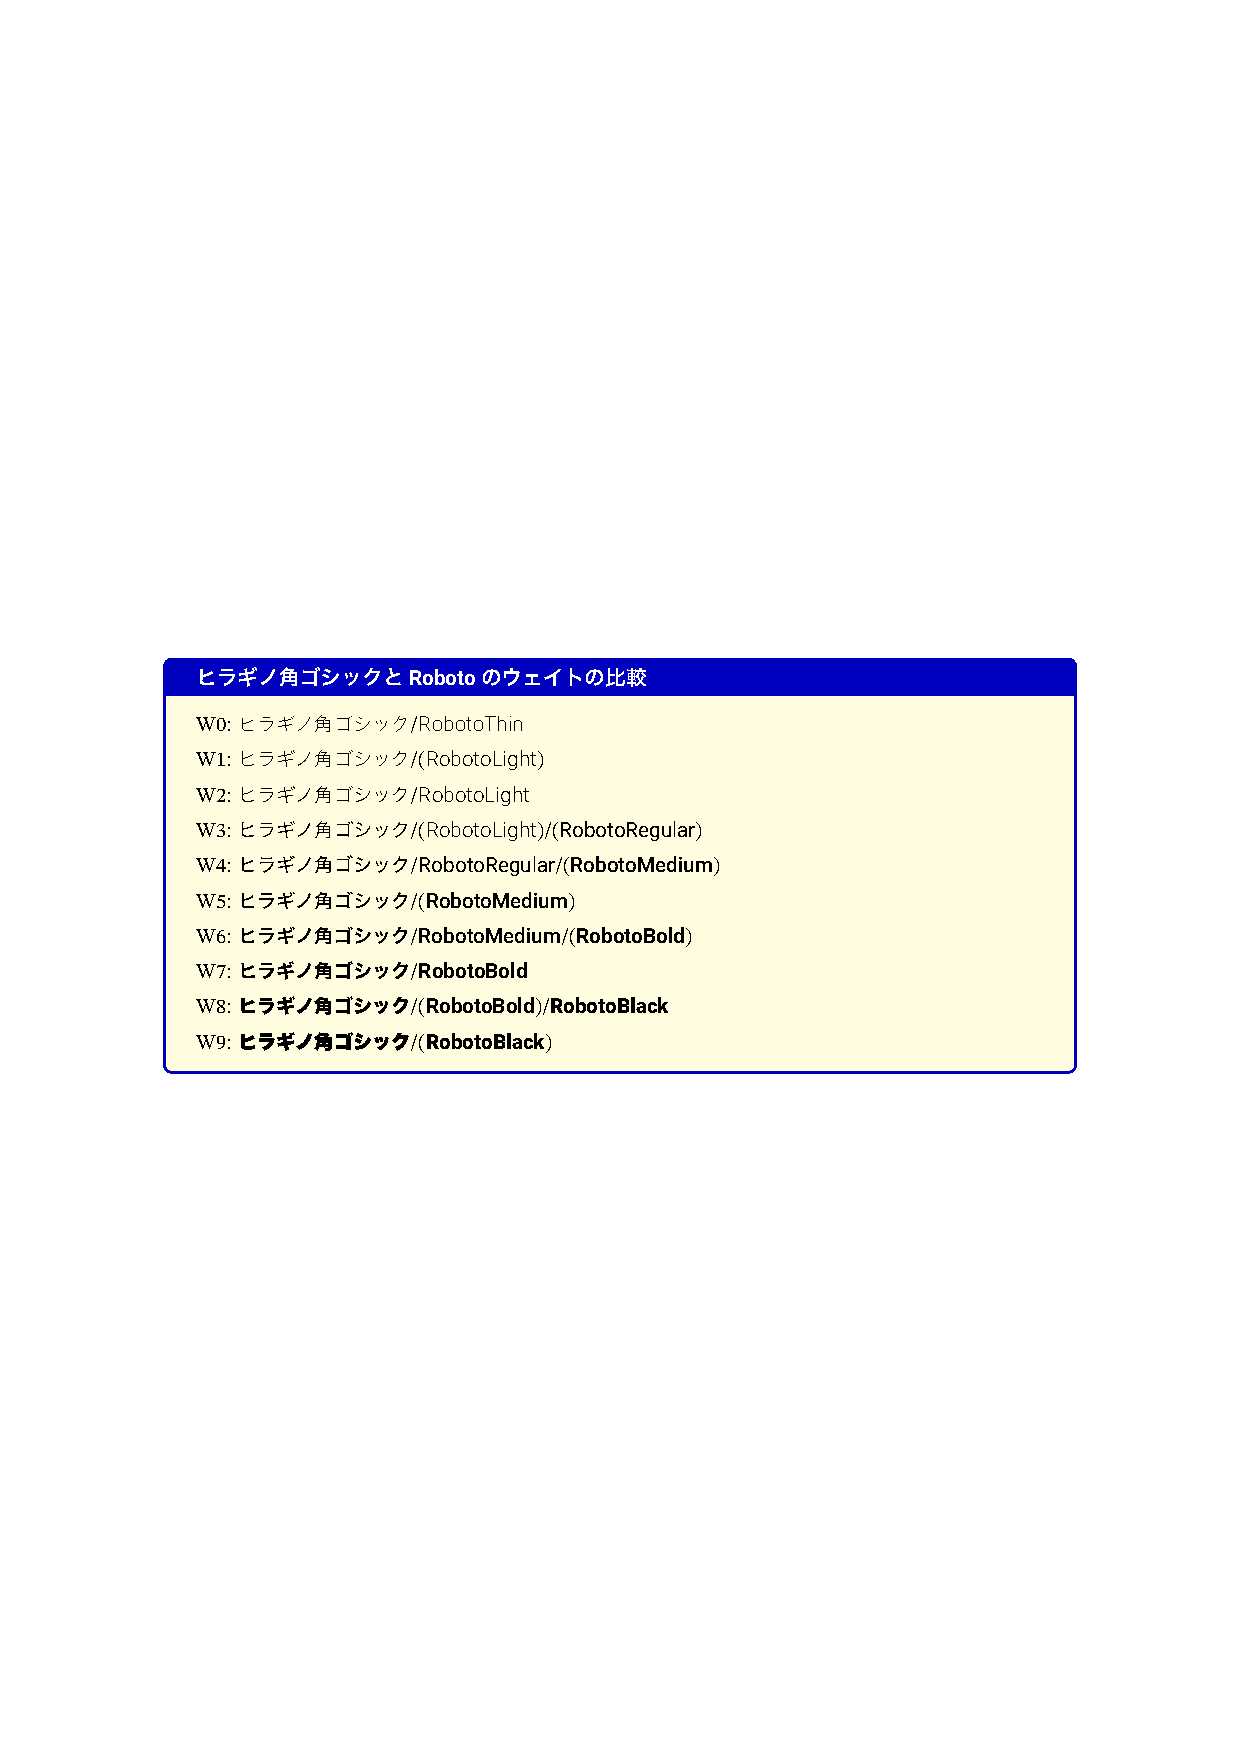
\includegraphics[scale=1.0,clip]{hira.pdf}
\label{hira}
\end{figure}
標準の設定では,通常フォントがヒラギノのW3とRobotoのレギュラー,太字では,ヒラギノのW6とRobotoのボールドが使用されるが,RobotoのレギュラーはヒラギノのW4とマッチし,ボールドはW7とマッチするように見える.
RobotoとSTIX Twoは同程度であるので,脚注\ref{太い}で,欧文フォントがヒラギノより若干太いのが気になると書いたが,実際そのとおりであることが確認できる.とはいえ,大きな差があるわけでもないので,気にしないならこのままでも問題ない.


\end{document} 